% thesis.tex
% This is the main file, which calls up preamble.tex, Frontmatterer.tex, and thesis.bib as needed.

% Frontmatter shortcuts; note the extr a space at the end, which is unfortunately necessary:
\newcommand\myname{Nathanael Aff }
\newcommand\mytitle{Improvement of Epsilon-Complexity Estimation and an Application to Seizure Prediction} 
% The graduate division requires this to be in caps.
\newcommand\mydegree{Master of Arts } % change to  Master of Science if applicable
\newcommand\myfield{Mathematics } % e.g., Mathematics
\newcommand\thismonth{August } % graduation month: May / August / \hhline{|=|=|=|=|=|}December
\newcommand\thisyear{2017 } % e.g., 201\graphicspath{{./figs/}}4

% \newenvironment{blue}{ \color{blue} }
% % preamble.tex, to be used with thesis.tex
% This contains the TeX definitions for layout, style, etc., as well as the first few pages of your thesis: title page, copyright page, approval page, abstract, acknowledgments, tables of contents, tables, and figures.
% The layout commands should give the correct margins according to the graduate division's guidelines

%%%%% TeX class and packages

\documentclass[12pt,oneside]{sfsuthesis}

% ==================================
% additional packages

\usepackage{amsthm,amsmath,amssymb,amsfonts,latexsym,graphicx,enumerate,setspace,verbatim,tocloft,rotating,color}

% =====================================
\usepackage[ruled,vlined]{algorithm2e}
\usepackage{hhline}
% \usepackage{algorithm}
\usepackage{algorithmicx}
% \usepackage{algpseudocode}
\usepackage{subcaption}
\usepackage{caption}
\usepackage{subfig}
\usepackage[export]{adjustbox}
\usepackage{float}

% \graphicspath{{./figs/}}

% ====================================

%\usepackage{color}                    % For creating colored text and background
%\usepackage{hyperref}                 % For creating hyperlinks in cross references
% other possibly useful packages: textcomp,mathrsfs,amscd,epsfig,euscript,cancel

%%%%% Layout
% These numbers might depend on your printer. Check the margins and compare them to the Graduate Division's
% guidelines. If there's something off, try playing with the numbers...
%
% For chapters:
%     Must have a minimum of 1.5in margin on left and 1in on all other sides.  Where there are page numbers
%     (whether on top or bottom), must have one additional inch between the page number and the text, for a
%     total of 2in between the edge of the paper and the text.
% For frontmatter pages:
%     The same margin numbers generally work, except for the Title Page, so you will notice that we use
%     some numbers for \textheight and \footskip right here, and then change them below, right after
%     generating the Title Page.

\hoffset=.5in 
\oddsidemargin=0in   % = 1in because LaTeX adds 1in
\evensidemargin=0in  % = 1in because LaTeX adds 1in
\topmargin=0in       % = 1in because LaTeX adds 1in
\headheight=0in
\headsep=1in         % Distance from top of pagenum (for page numbers at top-right corner of page) to text
\footskip=1.2in      % Distance from bottom of text to the page number (for page number at bottom of page)
\textwidth=5.9in     % Should be 6in, but use 5.9in to be conservative
\textheight=8.0in    % Best for Title Page (will change after the Title Page)

\pagestyle{plain}

\doublespacing

%%%%% Style of theorems, definitions, examples, equations, etc.

\theoremstyle{plain} % Heading is bold, text italic.
\newtheorem{theorem}{Theorem}[chapter]
\newtheorem{lemma}[theorem]{Lemma}
\newtheorem{proposition}[theorem]{Proposition}
\newtheorem{corollary}[theorem]{Corollary}
\newtheorem{conjecture}{Conjecture}[chapter]

\theoremstyle{definition}  % Heading is bold, text is roman
\newtheorem{definition}{Definition}[chapter]
\newtheorem{example}{Example}[chapter]

\theoremstyle{remark}  % Heading is italic, text is roman
\newtheorem*{remark}{Remark}
\newtheorem*{note}{Note}
\newtheorem{claim}{Claim}[chapter]

%%%%% Appendix style

\renewcommand\appendix[1]{
\chapter*{#1}
\addcontentsline{toc}{chapter}{#1}
}

%%%%% Title page

\begin{document}

\pagenumbering{roman}
\thispagestyle{empty}

\[ \]
\vspace{-1.9in}

\begin{center}
{\mytitle}

\vspace{1.4in}

\singlespace{A thesis presented to the faculty of\\
San Francisco State University\\
In partial fulfilment of\\
The Requirements for\\ The Degree}

\vspace{.5in}

\singlespace{\mydegree \\ In\\ \myfield}

\vspace{3.1in}

{by \\[12pt] 
\myname \\[12pt]
San Francisco, California\\[12pt]
\thismonth
\thisyear}
\end{center}

% \newpage
% \textheight=7.1in    % For all pages after the Title Page -- try making this number smaller (7.0 or 6.9) if the bottom margins are too small
% \footskip=1.1in      % Distance from bottom of text to the page number (for page number at bottom of page)
% \thispagestyle{empty}

% $\mbox{}$
% \vspace{3in}
% \begin{center}
% \singlespace{
% Copyright by\\ 
% \myname \\
% \thisayear
% }
% \end{center}

\newpage
\thispagestyle{empty}
\[ \]
\vspace{-1.8in}
\begin{center}
{CERTIFICATION OF APPROVAL}
\end{center}
\vspace{.6in}
\begin{quote}
I certify that I have read {\it \mytitle} by \myname and that in my opinion this work meets the criteria for approving a thesis submitted in partial fulfillment of the requirements
for the degree: \mydegree in \myfield at San Francisco State University.
\end{quote}

\vspace{0.75in}

\hspace*{\fill}\parbox{3.5in}{
\singlespace{

\hrule{\hspace{3.5in}} \\ 
Dr. Alexandra Piryatinska\\
Associate Professor of \myfield

\vspace{1in}

\hrule{\hspace{3.5in}} \\
Dr. Tao He\\
Assistant Professor of \myfield 

\vspace{1in}

\hrule{\hspace{3.5in}} \\
Dr. Chun Kit Lai\\
Assistant Professor of \myfield 

}
}

\newpage
\thispagestyle{empty}
\[ \]
\vspace{-1.8in}
\begin{center}
{\mytitle} \\

\vspace{.5in}

\singlespace{
\myname \\
San Francisco State University \\ 
\thisyear \\
}

\end{center}

\vspace{.3in}

\doublespacing{\noindent
The $\varepsilon$-complexity of a continuous function is a measure of the amount of information needed to reconstruct a function with an absolute error not larger than $\varepsilon$. For
H\"older class functions, $\varepsilon$-complexity is characterized by a pair of real numbers, the complexity 
coefficients.
The complexity coefficients have been shown to be useful features for the segmentation and classification of time series. 
In this work, we extend the set of
approximation methods used in estimating the complexity 
coefficients. The performance of these approximation methods is 
tested on a number of simulated time series.
% A set of simulations is used to test 
% the performance of this enlarged set of methods.
In addition, we test the conjecture that, for a given generating mechanism, the mean of the complexity coefficients is constant.
For our set of simulations, we find that the mean of the estimated complexity coefficients is constant on a constant H\"{o}lder class of functions. Finally, we apply the $\varepsilon$-complexity coefficients to the prediction of seizures in epileptic mice. 
% In particular, the $\varepsilon-$complexity coefficients are used to segment the EEG signal.   
%  Change points in the complexity coefficients are uased to 
%  segement the EEG signal and the average feature values on these
%  segments serve as predictors of a seizure outcome.
 We use this technique to identify which EEG signal preceded a seizure with over 80\% accuracy. 

}

\vspace*{\fill}

\hspace*{\fill}

\noindent
I certify that the Abstract is a correct representation of the content of this thesis.

\vspace{.6in} 

\hrule{\hspace{3.75in}} \\[-10pt]
Chair, Thesis Committee 
\hspace{2.5in}
Date

\newpage
\[ \]
\vspace{-1.8in}
\begin{center}{ACKNOWLEDGMENTS}\end{center}

\vspace{.3in}
\begin{quote}
\noindent
% I thank my advisor Dr. Alexandra Piryatinska her for her guidance 
% My two committee members Dr. Tao He and Dr. Chun-Kit Lai I thank 
% for their patience.

% And bicycle helmets off to
%  all my fellow students with whom I discussed math and problems of
 % other sorts over the last few years.
\end{quote}

\renewcommand{\contentsname}{\vspace{-1.8in} \begin{center} \normalsize \rm TABLE OF CONTENTS \end{center}}
\renewcommand{\listfigurename}{\vspace{-1.8in} \begin{center} \normalsize \rm LIST OF FIGURES \end{center}}
\renewcommand{\listtablename}{\vspace{-1.8in} \begin{center} \normalsize \rm LIST OF TABLES \end{center}}
\renewcommand{\cftchapfont}{\normalfont}
\renewcommand{\cftchappagefont}{\normalfont}
\renewcommand{\cftchapleader}{\cftdotfill{\cftdotsep}} % formatting commands for table of contents
\renewcommand{\cftsecfont}{\normalfont}
\renewcommand{\cftsecpagefont}{\normalfont}
\renewcommand{\cftsecleader}{\cftdotfill{\cftdotsep}}

\newpage \tableofcontents 
\newpage Table \hfill Page \listoftables % comment out if you don't use tables
\newpage Figure \hfill Page \listoffigures % comment out if you don't use figures

\newpage
\pagestyle{myheadings}
\pagenumbering{arabic} 
\setcounter{page}{1}

% %==========================================
% commands (naff)
%==========================================

\newtheorem{thm}{Theorem}[section]
\newtheorem{cor}[thm]{Corollary}
\newtheorem{lem}[thm]{Lemma}
\newtheorem{prop}[thm]{Proposition}
\theoremstyle{definition}
\newtheorem{defn}[thm]{Definition}
\theoremstyle{remark}
\newtheorem{rem}[thm]{Remark}
\numberwithin{equation}{section}


% M\alphaTH ****************************-
\newcommand{\R}{\mathbb R}
\newcommand{\eps}{\varepsilon}
\newcommand{\To}{\longrightarrow}
\newcommand{\B}{\mathbf{B}}
\newcommand{\A}{\mathcal{A}}
\newcommand{\Z}{\mathbb{Z}}
\newcommand{\C}{\mathbb{C}}
\newcommand{\Q}{\mathbb{Q}}
\newcommand{\N}{\mathbb{N}}
\newcommand{\F}{\mathbb{F}}
\newcommand{\FP}{\mathbb{P}}

\newcommand{\NC}{\mathcal{N}}
\newcommand{\BC}{\mathcal{A} }
\newcommand{\AC}{\mathcal{A} }
\newcommand{\HC}{\mathcal{H} }
\newcommand{\FC}{\mathcal{F} }
\newcommand{\CC}{\mathcal{C} }
\newcommand{\XC}{\mathcal{X} }
\newcommand{\GC}{\mathcal{G} }
\newcommand{\MC}{\mathcal{M} }
\newcommand{\LC}{\mathcal{L} }
\newcommand{\WC}{\mathcal{W} }
\newcommand{\VC}{\mathcal{V} }
\newcommand{\OC}{\mathcal{O} }
\newcommand{\DC}{\mathcal{D} }
\newcommand{\SC}{\mathcal{S} }
\newcommand\defeq{\mathrel{\overset{\makebox[0pt]{\mbox{\normalfont\tiny\sffamily def}}}{=}}}


\newcommand{\Ab}{\mathbf{A}}
\newcommand{\U}{\mathbb{U}}
\newcommand{\I}{\mathbb{I}}
\newcommand{\D}{\mathbf{D}}
\newcommand{\V}{\mathbf{V}}
\newcommand{\E}{\mathbf{E}}
\newcommand{\PB}{\mathbf{P}}
\newcommand{\ff}{\textbf{f}}
\newcommand{\uu}{\textbf{u}}
\newcommand{\vv}{\textbf{v}}
\newcommand{\ww}{\textbf{w}}
\newcommand{\xx}{\textbf{x}}
\newcommand{\yy}{\textbf{y}}
\newcommand{\btheta}{\mathbf{\theta}}

\newcommand{\bb}{\textbf{b}}
\newcommand{\nul}{\text{null }}
\newcommand{\range}{\text{range }}
\newcommand{\nsub}{\trianglelefteq}
\newcommand{\ndiv}{\hspace{-4pt}\not|\hspace{2pt}}
% Example with parameters
% \newcommand{\bb}[1]{\mathbb{#1}}
% norms, inner products,
\newcommand{\norm}[1]{\left\lVert#1\right\rVert}
\newcommand{\inner}[2]{\langle #1 , #2 \rangle}


% preamble.tex, to be used with thesis.tex
% This contains the TeX definitions for layout, style, etc., as well as the first few pages of your thesis: title page, copyright page, approval page, abstract, acknowledgments, tables of contents, tables, and figures.
% The layout commands should give the correct margins according to the graduate division's guidelines

%%%%% TeX class and packages

\documentclass[12pt,oneside]{sfsuthesis}

% ==================================
% additional packages

\usepackage{amsthm,amsmath,amssymb,amsfonts,latexsym,graphicx,enumerate,setspace,verbatim,tocloft,rotating,color}

% =====================================
\usepackage[ruled,vlined]{algorithm2e}
\usepackage{hhline}
% \usepackage{algorithm}
\usepackage{algorithmicx}
% \usepackage{algpseudocode}
\usepackage{subcaption}
\usepackage{caption}
\usepackage{subfig}
\usepackage[export]{adjustbox}
\usepackage{float}

% \graphicspath{{./figs/}}

% ====================================

%\usepackage{color}                    % For creating colored text and background
%\usepackage{hyperref}                 % For creating hyperlinks in cross references
% other possibly useful packages: textcomp,mathrsfs,amscd,epsfig,euscript,cancel

%%%%% Layout
% These numbers might depend on your printer. Check the margins and compare them to the Graduate Division's
% guidelines. If there's something off, try playing with the numbers...
%
% For chapters:
%     Must have a minimum of 1.5in margin on left and 1in on all other sides.  Where there are page numbers
%     (whether on top or bottom), must have one additional inch between the page number and the text, for a
%     total of 2in between the edge of the paper and the text.
% For frontmatter pages:
%     The same margin numbers generally work, except for the Title Page, so you will notice that we use
%     some numbers for \textheight and \footskip right here, and then change them below, right after
%     generating the Title Page.

\hoffset=.5in 
\oddsidemargin=0in   % = 1in because LaTeX adds 1in
\evensidemargin=0in  % = 1in because LaTeX adds 1in
\topmargin=0in       % = 1in because LaTeX adds 1in
\headheight=0in
\headsep=1in         % Distance from top of pagenum (for page numbers at top-right corner of page) to text
\footskip=1.2in      % Distance from bottom of text to the page number (for page number at bottom of page)
\textwidth=5.9in     % Should be 6in, but use 5.9in to be conservative
\textheight=8.0in    % Best for Title Page (will change after the Title Page)

\pagestyle{plain}

\doublespacing

%%%%% Style of theorems, definitions, examples, equations, etc.

\theoremstyle{plain} % Heading is bold, text italic.
\newtheorem{theorem}{Theorem}[chapter]
\newtheorem{lemma}[theorem]{Lemma}
\newtheorem{proposition}[theorem]{Proposition}
\newtheorem{corollary}[theorem]{Corollary}
\newtheorem{conjecture}{Conjecture}[chapter]

\theoremstyle{definition}  % Heading is bold, text is roman
\newtheorem{definition}{Definition}[chapter]
\newtheorem{example}{Example}[chapter]

\theoremstyle{remark}  % Heading is italic, text is roman
\newtheorem*{remark}{Remark}
\newtheorem*{note}{Note}
\newtheorem{claim}{Claim}[chapter]

%%%%% Appendix style

\renewcommand\appendix[1]{
\chapter*{#1}
\addcontentsline{toc}{chapter}{#1}
}

%%%%% Title page

\begin{document}

\pagenumbering{roman}
\thispagestyle{empty}

\[ \]
\vspace{-1.9in}

\begin{center}
{\mytitle}

\vspace{1.4in}

\singlespace{A thesis presented to the faculty of\\
San Francisco State University\\
In partial fulfilment of\\
The Requirements for\\ The Degree}

\vspace{.5in}

\singlespace{\mydegree \\ In\\ \myfield}

\vspace{3.1in}

{by \\[12pt] 
\myname \\[12pt]
San Francisco, California\\[12pt]
\thismonth
\thisyear}
\end{center}

% \newpage
% \textheight=7.1in    % For all pages after the Title Page -- try making this number smaller (7.0 or 6.9) if the bottom margins are too small
% \footskip=1.1in      % Distance from bottom of text to the page number (for page number at bottom of page)
% \thispagestyle{empty}

% $\mbox{}$
% \vspace{3in}
% \begin{center}
% \singlespace{
% Copyright by\\ 
% \myname \\
% \thisayear
% }
% \end{center}

\newpage
\thispagestyle{empty}
\[ \]
\vspace{-1.8in}
\begin{center}
{CERTIFICATION OF APPROVAL}
\end{center}
\vspace{.6in}
\begin{quote}
I certify that I have read {\it \mytitle} by \myname and that in my opinion this work meets the criteria for approving a thesis submitted in partial fulfillment of the requirements
for the degree: \mydegree in \myfield at San Francisco State University.
\end{quote}

\vspace{0.75in}

\hspace*{\fill}\parbox{3.5in}{
\singlespace{

\hrule{\hspace{3.5in}} \\ 
Dr. Alexandra Piryatinska\\
Associate Professor of \myfield

\vspace{1in}

\hrule{\hspace{3.5in}} \\
Dr. Tao He\\
Assistant Professor of \myfield 

\vspace{1in}

\hrule{\hspace{3.5in}} \\
Dr. Chun Kit Lai\\
Assistant Professor of \myfield 

}
}

\newpage
\thispagestyle{empty}
\[ \]
\vspace{-1.8in}
\begin{center}
{\mytitle} \\

\vspace{.5in}

\singlespace{
\myname \\
San Francisco State University \\ 
\thisyear \\
}

\end{center}

\vspace{.3in}

\doublespacing{\noindent
The $\varepsilon$-complexity of a continuous function is a measure of the amount of information needed to reconstruct a function with an absolute error not larger than $\varepsilon$. For
H\"older class functions, $\varepsilon$-complexity is characterized by a pair of real numbers, the complexity 
coefficients.
The complexity coefficients have been shown to be useful features for the segmentation and classification of time series. 
In this work, we extend the set of
approximation methods used in estimating the complexity 
coefficients. The performance of these approximation methods is 
tested on a number of simulated time series.
% A set of simulations is used to test 
% the performance of this enlarged set of methods.
In addition, we test the conjecture that, for a given generating mechanism, the mean of the complexity coefficients is constant.
For our set of simulations, we find that the mean of the estimated complexity coefficients is constant on a constant H\"{o}lder class of functions. Finally, we apply the $\varepsilon$-complexity coefficients to the prediction of seizures in epileptic mice. 
% In particular, the $\varepsilon-$complexity coefficients are used to segment the EEG signal.   
%  Change points in the complexity coefficients are uased to 
%  segement the EEG signal and the average feature values on these
%  segments serve as predictors of a seizure outcome.
 We use this technique to identify which EEG signal preceded a seizure with over 80\% accuracy. 

}

\vspace*{\fill}

\hspace*{\fill}

\noindent
I certify that the Abstract is a correct representation of the content of this thesis.

\vspace{.6in} 

\hrule{\hspace{3.75in}} \\[-10pt]
Chair, Thesis Committee 
\hspace{2.5in}
Date

\newpage
\[ \]
\vspace{-1.8in}
\begin{center}{ACKNOWLEDGMENTS}\end{center}

\vspace{.3in}
\begin{quote}
\noindent
% I thank my advisor Dr. Alexandra Piryatinska her for her guidance 
% My two committee members Dr. Tao He and Dr. Chun-Kit Lai I thank 
% for their patience.

% And bicycle helmets off to
%  all my fellow students with whom I discussed math and problems of
 % other sorts over the last few years.
\end{quote}

\renewcommand{\contentsname}{\vspace{-1.8in} \begin{center} \normalsize \rm TABLE OF CONTENTS \end{center}}
\renewcommand{\listfigurename}{\vspace{-1.8in} \begin{center} \normalsize \rm LIST OF FIGURES \end{center}}
\renewcommand{\listtablename}{\vspace{-1.8in} \begin{center} \normalsize \rm LIST OF TABLES \end{center}}
\renewcommand{\cftchapfont}{\normalfont}
\renewcommand{\cftchappagefont}{\normalfont}
\renewcommand{\cftchapleader}{\cftdotfill{\cftdotsep}} % formatting commands for table of contents
\renewcommand{\cftsecfont}{\normalfont}
\renewcommand{\cftsecpagefont}{\normalfont}
\renewcommand{\cftsecleader}{\cftdotfill{\cftdotsep}}

\newpage \tableofcontents 
\newpage Table \hfill Page \listoftables % comment out if you don't use tables
\newpage Figure \hfill Page \listoffigures % comment out if you don't use figures

\newpage
\pagestyle{myheadings}
\pagenumbering{arabic} 
\setcounter{page}{1}
  
% % draftpreamble.tex, to be used with thesis.tex
% This contains the TeX definitions for layout, style, etc., useful for the *draft* of your thesis.
% For the final version of your thesis, use preamble.tex

%%%%% TeX class and packages

\documentclass[12pt,oneside]{book}

\usepackage{amsthm,amsmath,amssymb,amsfonts,latexsym,graphicx,enumerate,setspace,verbatim,tocloft,rotating,color}

% =====================================
\usepackage[ruled,vlined]{algorithm2e}
\usepackage{hhline}
% \usepackage{algorithm}
\usepackage{algorithmicx}
% \usepackage{algpseudocode}
\usepackage{subcaption}
\usepackage{caption}
\usepackage{subfig}
\usepackage[export]{adjustbox}
\usepackage{float}
% Maintain apsect ratio

% \adjustbox{%
%     min size={\mywidth}{\myheight},%
%     Clip*={0.5\width - 0.5\mywidth} {0.5\totalheight - 0.5\myheight}%
%           {0.5\width + 0.5\mywidth} {0.5\totalheight + 0.5\myheight}%
% }{%
%     \includegraphics[max size={\mywidth}{\myheight}]{file.jpg}%
% }%


% =====================================
%\usepackage{color}                       % For creating colored text and background
%\usepackage{hyperref}                 % For creating hyperlinks in cross references
% other possibly useful packages: textcomp,mathrsfs,amscd,epsfig,euscript,cancel

%%%%% Layout

\voffset=-.8in 
\oddsidemargin=0in
\evensidemargin=0in
\textwidth=6.5in
\textheight=9in

\pagestyle{plain}

%%%%% Style of theorems, definitions, examples, equations, etc.

\theoremstyle{plain} % Heading is bold, text italic.
\newtheorem{theorem}{Theorem}[chapter]
\newtheorem{lemma}[theorem]{Lemma}
\newtheorem{proposition}[theorem]{Proposition}
\newtheorem{corollary}[theorem]{Corollary}
\newtheorem{conjecture}{Conjecture}[chapter]

\theoremstyle{definition}  % Heading is bold, text is roman
\newtheorem{definition}{Definition}[chapter]
\newtheorem{example}{Example}[chapter]

\theoremstyle{remark}  % Heading is italic, text is roman
\newtheorem*{remark}{Remark}
\newtheorem*{note}{Note}
\newtheorem{claim}{Claim}[chapter]

%%%%% Appendix style

\renewcommand\appendix[1]{
\chapter*{#1}
\addcontentsline{toc}{chapter}{#1}
}

%%%%% Comment command, useful for editing

\renewcommand\comment[1]{{\sc Comment:} {\bf #1}}

%%%%% Draft title page

\begin{document}

\thispagestyle{empty}

\[ \]
\vspace{1in}

\begin{center}
{\Large \bf \mytitle}

\vspace{1.5in}

\myname

\vspace{1.5in}

Version of \today

\end{center}

\newpage
\tableofcontents 
  


%==========================================
% commands (naff)
%==========================================

\newtheorem{thm}{Theorem}[section]
\newtheorem{cor}[thm]{Corollary}
\newtheorem{lem}[thm]{Lemma}
\newtheorem{prop}[thm]{Proposition}
\theoremstyle{definition}
\newtheorem{defn}[thm]{Definition}
\theoremstyle{remark}
\newtheorem{rem}[thm]{Remark}
\numberwithin{equation}{section}


% M\alphaTH ****************************-
\newcommand{\R}{\mathbb R}
\newcommand{\eps}{\varepsilon}
\newcommand{\To}{\longrightarrow}
\newcommand{\B}{\mathbf{B}}
\newcommand{\A}{\mathcal{A}}
\newcommand{\Z}{\mathbb{Z}}
\newcommand{\C}{\mathbb{C}}
\newcommand{\Q}{\mathbb{Q}}
\newcommand{\N}{\mathbb{N}}
\newcommand{\F}{\mathbb{F}}
\newcommand{\FP}{\mathbb{P}}

\newcommand{\NC}{\mathcal{N}}
\newcommand{\BC}{\mathcal{A} }
\newcommand{\AC}{\mathcal{A} }
\newcommand{\HC}{\mathcal{H} }
\newcommand{\FC}{\mathcal{F} }
\newcommand{\CC}{\mathcal{C} }
\newcommand{\XC}{\mathcal{X} }
\newcommand{\GC}{\mathcal{G} }
\newcommand{\MC}{\mathcal{M} }
\newcommand{\LC}{\mathcal{L} }
\newcommand{\WC}{\mathcal{W} }
\newcommand{\VC}{\mathcal{V} }
\newcommand{\OC}{\mathcal{O} }
\newcommand{\DC}{\mathcal{D} }
\newcommand{\SC}{\mathcal{S} }
\newcommand\defeq{\mathrel{\overset{\makebox[0pt]{\mbox{\normalfont\tiny\sffamily def}}}{=}}}


\newcommand{\Ab}{\mathbf{A}}
\newcommand{\U}{\mathbb{U}}
\newcommand{\I}{\mathbb{I}}
\newcommand{\D}{\mathbf{D}}
\newcommand{\V}{\mathbf{V}}
\newcommand{\E}{\mathbf{E}}
\newcommand{\PB}{\mathbf{P}}
\newcommand{\ff}{\textbf{f}}
\newcommand{\uu}{\textbf{u}}
\newcommand{\vv}{\textbf{v}}
\newcommand{\ww}{\textbf{w}}
\newcommand{\xx}{\textbf{x}}
\newcommand{\yy}{\textbf{y}}
\newcommand{\btheta}{\mathbf{\theta}}

\newcommand{\bb}{\textbf{b}}
\newcommand{\nul}{\text{null }}
\newcommand{\range}{\text{range }}
\newcommand{\nsub}{\trianglelefteq}
\newcommand{\ndiv}{\hspace{-4pt}\not|\hspace{2pt}}
% Example with parameters
% \newcommand{\bb}[1]{\mathbb{#1}}
% norms, inner products,
\newcommand{\norm}[1]{\left\lVert#1\right\rVert}
\newcommand{\inner}[2]{\langle #1 , #2 \rangle}

% \documentclass[thesis]{subfiles}

% \begin{document}
% main.tex, to be used with thesis.tex
% This contains the main work of your thesis.

% \include{}

\chapter{Introduction}

% Time-series arising 
% in biomedical contexts are often complex and have
% underlying mechanisms that are not well understood. 
% Applications of classification and clustering arise
% naturally in this context; 
% For example, time series collected 
% from the electrical potential generated by the heart -- 
% electrocardiograms (ECG) -- or by the collective 
% firing of synapses as captured by an 
% electroencephalogram (EEG), 
% or generated by direct measurements of human motion,
% are commonly used to monitor and classify the health 
% of patients. 
% time series. 
% Although in practice the line between diagnosiing 
% and modeling a biological process may not be 
% precise, the distinction is useful when considering
% what feature or model of a time series are of 
% interest, as it mirrors the trade off that 
% is often made between interpretation and 
% accuracy in modeling and predicting phenomena.
%  The purely diagnostic setting corresponds
% closely to the algorithmic task of classifying 
% signals
% ==================================
%  old 
% ==================================
% A common practice is to model these time series using
% parametric models for which assumptions made about the
% nature of the process generating the data. However, 
% biophysical time series are often complex, non-stationary
% or have non-linear characteristics.
% parameters for the model are often either iteratively 
% tuned or are restricted to a specific range based
% on domain knowledge. 


Many natural phenomena generate time series that
exhibit complex functional and statistical 
characteristics.
% exhibit complex characteristics which are readily 
% represented by  statistical models.
For example, an electroencephalogram(EEG) records
the electrical potential generated by the synchronized
firing of neurons. EEG signals are marked by both transient 
variations in waveforms and regime changes, distinct
breaks in the character and statistical distribution
of the EEG.
While the exact generating mechanisms of
variations in EEG may not be known, characteristics
 of the observed signal can be 
used to identify changes in the underlying dynamics.

The theory of $\varepsilon-$complexity as developed by 
Darkhovsky and Piryatinska provides a method
of identifying these regime changes
in complex signals such as EEG.
The definition of $\varepsilon-$complexity is related 
to Kolmogorov's definition of the complexity of a sequence.
Roughly, Kolmogorov identified the complexity
of a discrete sequence as the size of the program, or 
the amount of information, needed to produce that sequence. 
The $\varepsilon-$complexity of a continuous function, 
on the other hand, is the amount of information --- in this 
case, the proportion of the function, needed to reconstruct
that function with an absolute error not greater than 
$\varepsilon$. 
Darkhovsky and Piryatinska have shown that the 
$\varepsilon-$complexity of a continuous function 
can be identified by two real numbers\cite{darkhovsky2013}. 
These are the 
$\varepsilon-$complexity coefficients or simply the 
complexity coefficients of the function.
In practical applications, a signal like EEG is given by a
some finite set of samples. 
The theory of $\varepsilon-$complexity is adapted to a 
discrete setting by considering discrete sequences, such
as time series, as restrictions of continuous functions 
to a uniform grid.

The procedure for estimating the $\varepsilon-$complexity of 
a function entails the iterative approximation of that 
function on a smaller set of samples at each iteration. 
The initial implementation of the procedure for estimating $\varepsilon-$complexity coefficients
used piecewise polynomials to reconstruct to approximate the 
original function. We implement the estimation procedure with an enlarged set of approximation methods --- basis splines, cubic splines, and an interpolating subdivision 
method termed the lifting scheme. We test the estimation of 
$\varepsilon-$complexity on simulated data using each approximation
method. First, we compare the reconstruction accuracy of of 
each method. Then we test the performance of the complexity coefficients estimated with each approximation 
method when used to classify groups of related time series.
We also compare the computational efficiency of each 
approximation method. Although the basis spline method has the 
lowest approximation error across all simulations, we 
find that low approximation error does not correspond 
to improvements in classification accuracy. Each 
approximation method performs similarly in the classification 
task. However, the cubic spline method is the most computationally efficient, and is used to estimate the complexity coefficients in 
the applications discussed in Chapters 4 and 5.

Darkhovsky and Piryatinska have shown that for a H\"older class of functions the $\varepsilon$-complexity coefficients capture a linear relationship between the log of the approximation error and the log of the proportion of the function used in the approximation. They have conjectured that a 
constant generating mechanism corresponds to constant mean complexity coefficients. 
In Chapter 4 we use a number of simulations of deterministic and stochastic processes to test whether, on average, 
the complexity coefficients are constant for a 
constant H\"older class of functions. For these processes, a single parameter determines both the H\"older class and the fractal dimension of the time series generated
by the processes. For these simulations, the slope
complexity coefficient $B$ and an estimator
of fractal dimension behave simlarly as the parameters of
the processes are varied. For three of the four processes tested,
we find that the complexity coefficient $B$ is
on average, constant for a constant H\"older class of functions.
 
% The characteristics of an EEG signal can change rapidly over a short time period. Common classification methods use features averaged over arbitrary windows of time. 

In the final chapter, the complexity coefficients are applied
to the prediction of seizures in epileptic mice. Features from a 4 minute window of EEG are used to predict whether a stimulus
applied to epilepsy-prone mice will result in a seizure. 
% Most existing studies predict seizures with EEG data 
% from spontaneously occuring seizures. 
% For our study, we
A time series of length $n$ can be considered 
as a vector in an $n$-dimensional space. For example, 4 minutes of 
EEG from a single channel is a represented by 2 million 
observations.
A common method of handling such high dimensional data is 
to map the data to a lower dimensional set of features. For time series like EEG, features are often calculated 
on a uniform partition or on a sliding
window taken over the length of the signal. For an 
inhomogeneous time series like EEG, 
this may lead to features being calculated windows
with widely varying characteristics.
The $\varepsilon-$complexity 
was designed to identify such variations in a signal.
In order to calculate our features on more homogeneous 
time periods, we use change points in the 
complexity coefficients to segment the EEG.
The average value of features on these segments are then used as predictors of a seizure response. 

Models using this procedure to dynamically segment the EEG signal
are compared to several models which use features calculated on uniform partitions of the signal. 
For the best performing models, we are able to accurately classify 
seizure outcomes with over 80\% accuracy. A model with features calculated on uniform partitions performs 
as well or better than the models using changes in the complexity
coefficients to segment the signal.
Due to the small number of trials and some inherent limitations 
of the data, additional tests would be needed to 
know if how well the model performance reported here generalizes
to other contexts.


Finally, we have created an \texttt{R} language package, 
\texttt{ecomplex}, that implements 
the $\varepsilon$-complexity algorithm. The 
default settings of this package are based on the simulation 
experiments described in Chapter 3. Methods used 
for generating simulations, computing EEG features, 
and the classification algorithm used in Chapter 5 
have been also been included in \texttt{R} 
packages to enable further study or replication of
the experiments described in this work.

% \section{The lifting scheme}
% % In theory, the minimum 
% % estimation error at each step given any family 
% % of functions used to interpolate (or approximate)
% % the original function.
% In theory, the approximation error found at each 
% stage of the algorithm should be all possible 
% families of approximating functions.
%  In practice, 
% some well-defined family of functions is used.
% We implement the $\epsilon-$complexity 
% algorithm using two related 
% methods: basis splines (B-splines)and
%  wavelet splines. The wavelet splines 
%  are implemented using a computationally 
% efficient method called a lifting scheme\cite{sweldens}. 
% One motivation for 
% extending the family of approximating functions is 
% to minimize the approximation error at each 
% stage of the algorithm. Wavelet splines, though, are 
% essentially an iterated version of basis spline
% interpolation. That is, a single iteration of the 
% wavelet spline interpolation is equivalent to 
% interpolation using B-splines.
% The resulting reconstruction error does not differ
% significantly from the B-spline implementation. 
% However, the listing scheme 
% provides an time and space efficient method 
% for computing the interpolation. 

% % Since the spacing 
% % of the points used for interpolation are known 
% % at each stage of the algorithm a discrete time 
% %  filter can be computed before hand,
% % allowing for an efficient computation of the 
% % interpolated points.
% % (Specific claims f a faster implementation to 
% % be detailed later).


% % (transition)

% \section{Classification of EEG}

% % The $\epsilon$-complexity algorithm relies on
% % repeated reconstruction of the original data at  
% % coarser levels, or repeated downsampling of 
% % the data. This makes it best suited for 
% % densely sampled data. 

 
% % mice with a genetic disorder that makes them 
% % prone to epilepsy. 

% % (Explanation)
% The EEG signal measures the changes 
% in the brain's electrical field potential. 
% EEG signals are used in a range 
% of biomedical contexts, from diagnosing
% diseases of the brain to medical
% and commercial brain-computer applications.
% Traditional
% EEG analysis has focused on the spectral
% characteristics of the EEG signal. 
% A typical analysis characterizes a brain 
% state by the relative power within a given 
% frequency band. For example, low frequency 
% delta waves (0.5-4 Hz) and mid-frequency 
% alpha waves (8-12 Hz) have been associated 
% with distinct sleep stages.
%  However, EEG signals exhibit a range of 
%  complex characteristics. For example, 
%  EEG are non-homogeneous, non-stationary and have transient 
%  waveforms. \cite{pirya2009}
%  These
% characteristics make it difficult to analyze
% using standard parametric time series models.\cite{subha} 
% In addition to spectral characteristics 
% a range of features drawn from the study dynamic
% and non-linear systems -- fractional dimension, 
% correlation dimension, and higher order spectra
% have been used to study or classify EEG 
% signals.\cite{subha} 

% In this thesis we use a combination of these  
% features to study EEG signals of mice with 
% a genetic mutation that causes epilepsy. 
% We use the $\epsilon-$complexity algorithm 
% combined with spectral features and variance
% features to segment and classify the EEG 
% signals. In particular, we (attempt) to 
% predict the reaction of the mice to a stimulus
% intended to induce an epileptic reaction. 
% We use a change point algorithm to segment 
% data and then extract features from related 
% segments. The features drawn from this segmented
% data are then used to predict the post stimulus
% brain state of the mice.

% \section{The \texttt{ecomplex R} package}

% We have written an \texttt{R} package that includes 
% the $\epsilon-$complexity algorithm.  
% The package also the change point detection 
% algorithm used in our EEG analysis and  
% described in \cite{pirya2009}.[update] 
% A separate package includes code that 
% allows for the replication of our 
% analysis of synthetic time series and 
% mouse EEG data.


% We begin by outlining the motivation for the 
% $\epsilon-$complexity algorithm and we develop
% the mathematical theory of the procedure. We 
% review several features
% that aim to quantify 'complexity', 
% and describe their relation to the $\epsilon$-complexity
% feature. The mathematical background of 
% lifting scheme interpolation and it's relation to 
% wavelets is described along with the details 
% of the algorithm's implementation in the 
% \texttt{ecomplex} package. The new implementation 
% is tested on a set of synthetic data. Finally, 
% an analysis and classification of the 
%  the mutant epileptic mouse EEG 
% carried out using a change point algorithm and 
% a set of additional features including 
% measures of the variance and spectral content
% of the signal.





\chapter{Background}
  
  % In this chapter we introduce the definitions 
  % and notation that will be used in the following chapters. After 
  % a formal definition of $\varepsilon-$complexity we describe the 
  % procedure for computing


  % The sections on time series and approximation methods present basic background that someone familiar with the subjects could skip or refer back to as needed. 
  
\section{Epsilon-complexity} 
  
  % The term complexity has been used to describe diverse phenomena. The sensitivity of a dynamic system to initial conditions, 
  % the description length of a model, the unpredictability of a 
  %  sequence, the irregularity of a function or it's graph -- 
  %  a which the term complexity has been applied. 

  The word complexity has been used to describe a diverse set of both mathematical and natural phenomena. The use of the term to describe the complexity of a continuous
  function agrees with Kolmogorov's definition of the complexity of a discrete sequence. Kolmogorov 
  complexity characterizes the regularity of a
   sequence or string by the size of the program needed to output that sequence. For example, we can take as our sequence a natural number and let our 'program' or representation of that number in scientific notation.
    Then we can express 1,000,000 in 2 digits as 1E6 while the prime 7919 could not be similarly compressed \cite{vitanyi1993}. In this case, 1,000,000 is less complex 7919. 
  The approach taken by Darkhovsky and Piryatinska in defining the $\varepsilon$-complexity of a continuous function takes inspiration from Kolmogorov's definition of complexity\cite{darkhovsky2013}. 
   The information, roughly speaking, contained in a continuous 
   function is measured by the number of points sampled from the function that is needed to reconstruct that function within some error $\varepsilon$. 
   The algorithm used to compute $\varepsilon-$complexity coefficients makes successive approximations of
   a function with fewer and fewer sampled points. The two $\varepsilon$-complexity coefficients parametrize the linear 
   relationship between 
   the log of the approximation error and the log of the proportion 
   of points for each successive approximation.

  % \begin{defn}{Kolmologrov Complexity}\label{def:kolmogorov1}
  %   The Kolmogorov complexity of a sequence $a(t)$, denoted $K(w)$ 
  %   is the shortest program that outputs $a(t)$.
  % \end{defn}
  % -------------- edit above ----------------
  % } % end blu
  
  We begin with the formal definition of the $\varepsilon-$complexity of a single function followed by the primary theorem of \cite{darkhovsky2013} which shows that $\varepsilon-$complexity  characterizes the H\"older condition of a class of functions. The practical computation of $\varepsilon-$complexity takes a slightly different form than that used in the proof of this theorem and we describe this difference and present the algorithm used to compute the $\varepsilon-$complexity coefficients in practice. 

  % Throughout this thesis we will be referring to continuous 
  % functions, stohastic processes and observed time series 
  % and in 

% begin edit -------------------------------------------------------
   Although the original theory of 
  has been developed for the more general case of vector-valued 
  functions, we restrict this presentation to the case of 
  univariate functions.
  Let $x(t)$ to be a positive continuous function defined on the 
  unit inverval $ \mathbb{I} = [0,1]$. Let $\norm{\cdot}$ be a norm on the function and we can assume $\norm{x(t)} = 1$, that is, the function has been normalized 
  by taking $x(t)/\norm{x(t)}.$ Given some family of approximation 
  methods $\mathcal{F}$, let $\hat x(\cdot)$ be an approximation
  of $x(t)$ reconstructed from regularly samples spaced at intervals $h$. Then the absolute recover error function is defined 
  \begin{align}
    \delta^{\mathcal{F}}(h) = \inf_{\hat x \in \mathcal{F}} 
    \sup | x(t) - \hat x(t)|
  \end{align}
  % We note that $\delta^{\mathcal{F}}$ is a function of $h$.  

  % We will assume that $x(t)$ does not permit a perfect 
  % reconstruction for any $\hat x(\cdot) \in \mathcal{F}.$
  \begin{align*}
    h_x^*(\varepsilon, \mathcal{F}) = \begin{cases}
      \inf \{ h \leq 1 : \delta^{\mathcal{F}}(h) > \varepsilon \} & \text{if} 
      \{ h : \delta^{\mathcal{F}}(h) > \varepsilon \} > 0  \\ 
        1, &  \text{if no such } \hat x(t) \in \mathcal{F} \hspace{1em}\text{exists.}
    \end{cases}
  \end{align*}
  In words, the function $h^*(\varepsilon, \mathcal{F})$ is the minimum grid spacing $h$, or sample density, needed to approximate $x(t)$ within $\varepsilon$. 
  \begin{defn}{\textbf{Epsilon-complexity.} }\label{def:ecomplexity}
  The number
  \begin{align}
        % \begin{align}
  %   -\log h_x^*(\varepsilon, \mathcal{F}) \approx 
  %   \mathcal{A} + \mathcal{B}\log \varepsilon.
  % \end{align}
    \mathbb{S}_x(\varepsilon, \mathcal{F}) =  
    -\log h_x^*(\varepsilon) 
    \mathcal{F})
  \end{align}
  is the $(\varepsilon, \mathcal{F})-$complexity, 
  or simply, $\varepsilon-$complexity of the function $x(\cdot)$. 
  \end{defn}

  We will be referring variously to the H\"older condition or 
  H\"older continuity of a function which we now define:
  \begin{defn}{\textbf{H\"older Continuity.} }\label{def:holder}
    A function $x(t)$ is said to be H\"older continuous if
  there exists non-negative constants, $C, \alpha$ such that 
  \[
      |x(t) - x(s)| \leq C\norm{x -s}^{\alpha}
  \]
    for all $t$ and $s$.
  We refer to this as the H\"older condition with H\"older 
  exponent $\alpha$ or say a function is H\"older $\alpha$.
  \end{defn}
   Darkhovsky and Pirytinska have show that for almost any
  individual H\"older class function and given a rich 
  enough family of approximation methods  
  then the epsilon complexity has an approximately linear
  relationship to $\log \varepsilon$\cite{darkhovsky2013}
  \begin{align} \label{eq:linear-ecomplex}
      -\log h_x^*(\varepsilon, \mathcal{F}) \approx \mathbb{A} + 
    \mathbb{B}\log \varepsilon.  
  \end{align}
  
  The relationship serves the basis, after rearrangement, 
  for the estimation of $\varepsilon$-complexity for 
  discrete time series.
  In practial applications any function or time series 
  is acquired as some discrete set of samples, which we
  will assume to be taken at regular intervals. We 
  consider this discrete set to be a continuous function
  restricted to a uniform grid. In this case, 
  $h*(\epsilon, \mathcal{F})$, which we simplify here to 
  $h^*(\epsilon)$, is the proportion of sampled points
  and $\frac{1}{h^*(\varepsilon)}$ is the 
  number of points needed to approximate some function $x(t)$ within 
  $\varepsilon$. Let $n$ be the total number of points 
  in the initial sampling, then we denote the 
  proportion of points needed for reconstruction with 
  $\varepsilon$ 
  \begin{align}
     S(\cdot) \defeq \frac{n}{h^*(\varepsilon)}.
   \end{align} 
   \begin{defn}
     The $\varepsilon-$complexity of a function 
     given represented by a set of values sampled on 
     a uniform grid is $-\log S(\cdot)$.
   \end{defn}
  It follows from defintion \ref{def:ecomplexity} that
  \begin{prop}
    \[
      -\log S(\varepsilon, \mathcal{F}) \to \mathbb{S}_x(\varepsilon, \mathcal{F}) 
    \]
    as $n \to \infty$.
  \end{prop}
  For the discrete case, rearrangement of the relation \ref{eq:linear-ecomplex} gives and substitution of $\log S$ for $\mathbb{S}_x(\varepsilon, \mathcal{F})$ gives us the relation
  \begin{align}\label{eq:discrete-ecomplexity}
     \log \varepsilon  \approx A + B \log S.
   \end{align} 
  For practical computations, some set number of grid spacings 
  $h$ corresponding to the proportion $S_h$ are used to 
  estimate the linear relation in \ref{eq:discrete-ecomplexity}. 
  For each spacing $h$ we find the minimum error approximation 
  at that spacing.
  The parameters of this linear relationship, $A, B$, are the 
  $\varepsilon-$complexity coefficients or simply the  
  complexity coefficients. 

%-------------------------------- End edit
  


  In practical applications, a given function $x(t)$ is of some finite length $N$ and we assume the function has been sampled on some regular grid $\Z_h$.  The given initial sampling grid determined by $h_1$ is the densest resolution of the function and other grid spacings $h_2, h_3, ..., h_d$ are also taken at regular intervals.  
  For each $h_k$ the function $x(t)$ is approximated 
   with some family of methods
    $\mathcal{F}$. For a given $h$ the minimum mean-squared error
   is then added to the set of errors, 
   $\varepsilon_{\mathcal{F}, h}$. 
   Finally, setting $S_h = \frac{1}{h}$, a least squares linear model is fit to the set of errors   $ \{ \varepsilon_{\mathcal{F}, h} \}$ regressed on the proportion of function values 
   $\{ S_h \} $:
  \[
      \log  \varepsilon_{\mathcal{F}, h} 
      \sim A + B \log S_h.
  \]
  The parameters of the linear model $A, B$ are the 
  $\varepsilon-$complexity coefficients or simply the  
  complexity coefficients.

   \begin{algorithm}[htb]
    \label{alg:ecomplexity}
  \caption{$\varepsilon-$complexity \label{alg:ecomplex}}
  \DontPrintSemicolon
  \SetAlgoLined
  \SetKwInOut{Input}{Input}\SetKwInOut{Output}{Output}
  \Input{$X$ a regularly sampled time series of length $N$.} 
  \Input{$ \mathcal{F} $ a set of approximation methods $f$.}
  \Input{$ \mathcal{H} $ the set of spacings $h$.}
  \Output{The complexity coefficients $A,B$.}
  % \tcp{initialize array}
   % Initialize the array epsilons $\leftarrow [0]$   \;
  \BlankLine 
 \ForEach{$h$ in $H$} {    
    % \tcp{initialize array}    
    % mse $\leftarrow [0]$ \;
    \ForEach{$f$ in $\mathcal{F}$} {
      % \tcp{Compute the approximation error}
        Compute the approximation error \\ 
        $\varepsilon_{h,f} \leftarrow 
       \frac{1}{N}\norm{f_h - X_{h} }^2$.  \;
      % mse\leftarrow \varepsilon_{h,f}$
    } 
     Find minimium error over all $f$  \\
     epsilons$_h$ $\leftarrow \min \varepsilon_{h,f}$. \;
  }
  Fit a least squares linear model \\
   $A,B$ $\leftarrow$ lm($\{$ epsilons$_h$ $\}$ $ \sim \{ S_h \} $.) \;
  \end{algorithm}

% \caption{$\varepsilon-$complexity}

%   \end{algorithm}
% \usepackage[ruled,vlined]{algorithm2e}


\section{Time series}
  
  % We now describe some basic properties of time series or stochastic processes. 
  The theory 
  of $\epsilon-$complexity as developed by in \cite{darkhovsky2013} for continuous and possibly vector-valued functions 
  denoted $x(t)$. For the remainder of this thesis of our discussion will be restricted primarily to functions on $\R^1$, or univariate stochastic processes which we also refer to as time series. 
  % which we will refer to as a time series.
  % We touch briefly on more general random processes at the end of this section but will not go into the theory of more general processes in any detail. 

  A time series is a stochastic process, or set of random 
  variables, $X(t)$ or $X_t$, parametrized by time, 
  $\{ X_t: t \in T = \{ 1,2,3,... \}\}$.  
   We will denote realizations of a time series
   with the lower case 
  $x_t$ or $x(t)$. We also use $x(t)$ to refer to a continuous function or samples from the continuous function and we will not always distinguish between samples from a continuous function and observations of a random process. 

  We will begin by defining several 
  properties of time series 
  We also introduce a number of time series model
  that are used in the following chapters to 
  generate time series on which we 
   test the behavior of our implementation 
  of the $\varepsilon$-complexity algorithm. 
  Several of models we introduce have known 
  properties such as H\"older class and fractal 
  dimension and we test if and how the complexity coefficients
   measure these properties in Chapter 4.

  The ARMA model is a simple and widely used parametric time series model. It is a linear model
  that combines autoregressive (AR) and moving average (MA)
  models. The AR component expresses an observation at time 
  $t$ as a linear combination
  of preceding observations plus a random error component:
  \begin{align}
      X_t  = b_1 X_{t-1} + \cdots + b_p X_{t-p} + \varepsilon_t
  \end{align}
  
  The number of previous observations $p$ is the order of the 
  model, denoted $AR(p)$. The random error, $\varepsilon_t$, 
  is assumed to be independent, identically distributed (IID) observations from white noise a standard normal distribution with 
  mean 0, variance $\sigma^2$ and covariance 
  $Cov(X_i, X_j) = 0, i \neq j$. The latter is called 
  white noise and the errors are said to be 
  drawn from a white noise process 
  $\{ \varepsilon_{t_i}, \varepsilon_{t_j}\} \sim WN(0, \sigma^2)$. 

  The moving average(MA) process of order $q$ models
  the observation $x_t$ as a linear combination of $q$
  samples $\{ \varepsilon_t \} \sim WN(0, \sigma^2)$  
  \begin{align}
      X_t = \varepsilon_t + a_1 \varepsilon_{t-1} + 
    \cdots + a_q \varepsilon_{t-q}.
  \end{align}

  Depending on the parameters $p,q$ of an 
  ARMA$(p,q)$ process, 
  the resulting time series may or may not be 
   \textit{stationary}. A strictly stationary 
   time series is one 
   whose distribution independent of time $t$. 
   We will be using the term to indicate 
   a \textit{weakly stationary} time series, or 
   a time series whose first two moments do not 
   depend on time.
  %  A \textit{strongly stationary} 
  % have the same joint distribution $\{X_t, X_{t+ k} \}$ for 
  % all $k$. First, we define the following terms:
  % [check]
  % \begin{defn}\label{eq:mean_function}
  % [Notes : correllation -> standardized covariance make explicit.]
  % A \textit{weakly stationary} time series. 
  \begin{defn}\label{def:stationary}{\textbf{Weak stationarity} }
   A  \textit{time series} with finite variance and a 
  mean $\mu_t$ that does not depend on time is called 
   \textit{weakly stationary}: 
  \begin{align*}
    &\mathop{E}(X_t^2) < \infty \\
    &\mathop{E}(X_t)  = \mu \hspace{1em} \text{is a constant 
    independent of t }\hspace{1em} \\
    &\text{Cov}(X_t, X_{t+ h }) \hspace{1em}\text{ is independent
    of } t \text{ for each } h\hspace{1em}.
  \end{align*}   
  \end{defn}
   Where it exists, let $\mathop{E}(X_t)  = \mu_{t}$ be the mean function of a time series.
  %   \begin{align*}
  %      = \int_{-\infty}^{\infty} X f_t(X) dt.
  %   \end{align*}
  %  where $\mathop{E}$ is the expected value operator. 
  % \end{defn}
  \begin{defn}{\textbf{Covariance function.}} 
  \label{eq:auto_covariance}
  The  \textit{autocovariance or covariance} of a time series with mean $\mu$ 
  is then defined
  \begin{align*}
    \sigma(h) = \text{Cov}(X_{t}, X_{t + h})
                = E[(X_{t}-\mu_t)(X_{t + h} - \mu_{t + h})]  
   \end{align*}
   In the case of a zero mean function this simplifies
   \begin{align*}
      \sigma(h) = E[(X_{t})(X_{t + h}]).  
   \end{align*}
    The \textit{autocorrelation} function of $X_t$ is
    \begin{align*}
       \rho(h) \equiv \sigma(h)/\sigma(0) \equiv \text{Corr}(X_{t + h}, X_t), 
       \hspace{2em} h \in \{ 1,2,3,... \}.
     \end{align*} 
  \end{defn} 
  For a stationary, mean zero stochastic process with 
  $\sigma^2 = 1$ the autocorrelation and autocovariance function 
   are equivalent. Some stochastic
  processes, like the Cauchy process we introduce later, 
  can be specified by entirely by their autocorrelation function. 
  
  If a stationary process has an absolutely summable 
  autocovariance function
  \[
  \sigma(h), \sum_{-\infty}^{\infty}|\sigma(h)| < \infty
  \] then the
   \textit{spectral density function} of the process 
   is the Fourier transform of the $\sigma(h)$
   \begin{align}
      f(\omega) =  \sum_{-\infty}^{\infty} e^{2 \pi i \omega h} f(\omega)d \omega \hspace{1em}  -1/2 \leq \omega \leq 1/2.
    \end{align}
  Conversely, $\sigma(h)$ can be represented as
   the inverse transform of 
  the spectral density function. In either case, the two 
  representations carry the same information about the process.

  A stationary ARMA process has an autocorrelation  
  function $\rho(h)$ that decays at an exponential rate 
  as $|h| \to \infty$ \cite{fan2003}. A slowly decaying 
  autocorrelation function is characteristic of 
  a non-stationary process with long-range dependence. 
  We include three functions in our set of simulations that can have long-range dependence -- fractional Brownian motion, the Cauchy process and the fractionally integrated ARMA or FARIMA process. 
  The first two of these we discuss in the next section. 
  The ARIMA process is model whose integral 
  differences $d$ are a ARMA(p,q) processes,
  denoted ARIMA$(p,d,q)$.  
  The FARIMA model is a modifies ARIMA process
  allowing for fractional values $d$\cite{fan2003}.

   
  % The combined ARMA model of order $p,q$, ARMA$(p,q)$, is
  % thena
  % \begin{align*}
  %   X_t = b_1 x_{t-1} + \cdots + b_p x_{t-p} + 
  %   \varepsilon_t + a_1 \varepsilon_{t-1} + 
  %   \cdots + a_q \varepsilon_{t-q}.
  % \end{align*}
  % % def
  % The \textit{backshift operator} $B$ is defined 
  % \begin{align}\label{eq:backshift}
  %   B^kX-t = X_{t-k}, \hspace{2em} k \in \{ 1,2,3, ... \}
  % \end{align}   
  % and the polynomials AR and MA polynomials 
  % $a(\cdot)$ and $b(\cdot)$
  % \begin{align}\label{eq:arma_polynomials}
  %   b(a) = 1 - b_1z - \cdots - b_p z^p, \hspace{.5em} 
  %   a(z) = 1 + a_1z + \cdots + a_qz^1. 
  % \end{align}
  % \begin{defn}\label{defn:arma}
  %  A time series $X_t$ is defined to be an ARMA$(p,q)$ process 
  %  \begin{align*}
  %     b(B)Z_t = a(B)\eps_t.
  %   \end{align*} 
  % where $b(\cdot)$ and $a(\cdot)$ are the AR and MA polynomials
  % respectively. 
  % \end{defn}

  %  The ARIMA model 
  % has first differences, $x_t - x_{t-1}$, that come 
  % from an ARMA model. Before defining an ARIMA process we introduce 
  % some notation and present a simple example of a non-stationary 
  % time series.
   
  % A random walk defined
  % \begin{align*}
  %     Y_t & = Y_{t-1} + \eps_t \hspace{2em} \eps_t 
  %     \sim WN(0, \sigma^2)
  % \end{align*}
  % is not stationary. We define the differencing operator
  % \begin{align}\label{eq:difference}
  %   \nabla^dX_t &= (1 - B)^dX_t
  % \end{align}
  % where $B$ is the backshift operator. Then taking 
  % the first difference of the random walk $Y_t$
  % results in a stationary time series
  % \[
  %   \nabla^d Y_t =  (1 - B)x_t =  x_t - x_t - \eps_t = \eps_t,
  % \]
  % since $\eps \sim WN(0, \sigma^2)$.  

  %  The \textit{autoregressive integrated moving 
  % average}(ARIMA) \textit{process} is a model of time series
  % whose first or higher order differences are ARMA$(p,q)$ 
  % processes.
  % \begin{defn}\label{defn:arima}
  %   A time series $X_t$ is an ARIMA$(p,d,q)$ process if 
  % \begin{align*}
  %   \nabla^dX_t &= (1-B)^d X_t \hspace{1em} d \in \{ 1,2,3, ... \}.
  % \end{align*}
  % \end{defn}
  
  % An ARIMA model with  $d\in (-0.5, 0.5)$. 
  % \[
  %    \nabla^dX_t = \eps_t, \hspace{2em} \{ \eps_t \} 
  %    \sim WN(0, \sigma^2)
  % \]
  % is called  \textit{fractionally integrated noise} for 

  % % (Example Picture)
  % For a stationary ARMA processes, the observation 
  % of the observation $x_t$ has a finite dependence 
  % on previous observations 
  % $\{ x_{t- 1}, x_{t- 2} , ... \}$. (The autocorrelation
  % decays to zero relatively quickly):
  % \[
  %     |\rho(k)| \leq Cr^k, \hspace{1em} k = \{ 1,2,... \}.
  % \]  
  % These are termed short memory processes. A long 
  % memory process .... 
  % \[
  %   \rho(k) \sim Ck^{2d -1} \hspace{1em}\text{as }\hspace{1em}
  %   k \to \infty
  % \]
  % where $C$ is a positive constant and $d < 0.5$.
  % Such processes whose ACF are not absolutely 
  % summable are called  \textit{long memory processes}. 
  % (Such processes are found in biology, (famously the stock market)).  


% (DELETE)
%   (FARIMA definition).

%   A simple example of a non-stationary time series is one with a linear trend, but time series can exhibit more complex types of non-stationarity. For example, 
%   the mean of the time series may vary in some non-linear
%   fashion or the variance (or higher moments) of the time series may be time-dependent. An MA process of finite order is stationary since it is a weighted sum of white noise with mean 0. However, whether an AR model of finite order is stationary depends on its parameters. 


  % For ARMA models 
  % in particular, the parameters of an ARMA model 
  % can specify a non-stationary model. For example, 
  % if the sum of the coefficients of a moving average
  % model is not finite, then 

 % Other nonlinear 
 %  features are non-normality of the observed data, 
 %  nonlinear dependence of the observed values on past
 %  values, transient or asymmetric cycles and sensitivity
 %  of a model to its initial conditions. 
 %  % Example
 %  \cite{fan2003}\cite{pirya2009} 
  % There is some ambiguity, 
  % however, in the terms ''nonlinear'' or ''complex'' are 
  % used, as they may refer to either property of 
  % an observed time series, the probabilistic model 
  % of the time series, or of a mathematical model 
  % of the underlying process.


  % In a range of parametric models have been created that
  % capture these more complex or nonlinear features of 
  % a time series. For example, ARIMA models modify the 
  % ARMA model to capture trends, ARCH models are 
  % used to model time-dependent variance and a FARIMA 
  % process models large-range dependence or a\textit{long memory}
  % processes. 
  
  % We have introduced these models to define some terminology and present the ARMA model that will be used later in a simulation study of the performance of $\varepsilon-$complexity in classifying time series. We are also presenting the motivating context for the development of time series features like $\varepsilon-$complexity. When a time series is modeled by some parametric process assumptions are made about the nature of the stochastic process. These assumptions may be based on an understanding of the physical process generating the time series or on past modeling performance. In some cases, however, properties of either the physical process may not be well-understood, or a time series may exhibit complex features that aren't easily captured by a parametric model. The
  % $\varepsilon-$complexity feature is one among a number of features that have been developed to characterize time series that exhibit these complex features. A 
  % number of other features were developed to quantify time series complexity in the context of the study of dynamic systems. In the next section describe some of these features why they were developed.
  % % possibly add (FARIMA) 

% MACKEY GLASS

% In addition to these, the  \textit{Mackey-Glass}  equation and 
% the random-phase Weierstrass function were used in the tests. 

% The Mackey-Glass equation is a nonlinear delay 
% differential equation 
% \begin{align*}
%    \frac{dx}{dt}  = \beta \frac{ x(t - \tau) }{1 + x(t - \tau)^n } - 
%    \gamma x(t) \hspace{1em} \gamma, \beta, n > 0.
% \end{align*}
% where $\tau$ is the time delay of the system. The equation 
% has been used to model physiologial processes with feedback with 
% a feedback system. (See Scholarpedia -- infinite dimensional 
% attractor ?  why it's been used as a system for algorithms 
% that characterize dynamical systems.) 

% \textit{Notes on Mackey-Glass.} A discrete differential equation
% was used to approximate the Mackey-Glass equation. In our tests, 
% noise was added to equation (SNR ratio) since the function 
% simulated function was relatively smooth and was easily
% differentiated by the $\varepsilon-$coefficients. 
% [Revise]

\section{Fractal dimension}

In the following chapter, we test the 
relationship between the H\"older continuity 
of a function, estimators of its fractional or fractal
dimension and 
the $\varepsilon-$complexity coefficients. Here we define 
fractal dimension and introduce several 
functions or stochastic processes with known fractal 
dimension.

Although fractal dimension is a general measure on sets
we will be considering only those sets formed by the 
graph of a function $f$ or a sample function 
drawn from a stochastic process. Fractal dimension 
coincides with the usual sense of 
dimension for smooth manifolds such as the interval 
$[0,1]$. Since we consider only graphs
 $\Gamma:\{ (x, f(x)) \}$ in $\R^2$
the fractal dimension of these graphs should take on 
values between $[1,2)$.
% Let $f$ be a function, $f: \R \to \R$, then the graph of the 
% function is defined $\Gamma:\{ (x, f(x)) \} \in \R^2$. 
% Although we discuss two measures of fractal dimension in 
% some cases we will not distinguish between the types of 
% fractal dimension, for example, when we discuss estimators
% fo fractal dimension. 

The Hausdorff dimension of a set $E$, roughly speaking, 
measures the size of covers of that set 
as the diameter of covering elements
$\{ U_i \}$ approaches zero. We define the diameter 
of a set $U$ denoted $|U|$ as 
$\sup \{ | x- y| : x, y \in U\}$, the greatest distance 
between any two points in the set. A set collection 
$ \{ U_i \}$ is 
a cover of $E$ if $E \subset \bigcup_i^{\infty} U_i$
where we assume $\{ U_i \}$ is countable. 

\begin{defn}{\textbf{Hausdorff Dimension} }
Let all elements in $ \{ U_i \}_{\delta}$ be a
countable subset of $\{ U_i \}$ with diameter greater 
than $\delta$ such that $\{ U_i \}_{\delta}$ cover 
some set $E \subset \R^n$. The the Hausdorff dimension 
$\mathcal{H}_{\delta}^{\alpha}$ for any $\delta > 0$ 
is defined 
\begin{align*}
  \mathcal{H}_{\delta}^{\alpha} = \inf 
    \left[ \sum_i | U_i |^{\alpha} : \{ U_i \} \hspace{0.5em}\text{ is  a cover of  }\hspace{0.5em} E \right].
\end{align*}  
Then 
$$
\mathcal{H}_{\alpha(E)}=\lim_{\delta\to 0} H^{\alpha(E)}_\delta
$$

% $\mathcal{H}^{\alpha}(E) = 
%  \lim $ as $\delta \to 0$ of $ \mathcal{H}_{\delta}^{\alpha}$.
\end{defn}

For $0 < \alpha < 1$, $\mathcal{H}^{\alpha}$ is 
either $0$ or $\infty$ and there exists a critical point 
$\alpha$ at which $\mathcal{H}^{\alpha}$ switches from $0$ to 
$\infty$. This point is the Hausdorff dimension of the set 
which we denote $\dim_H E$ \cite{falconer2003}. 

% We consider two version of fractal dimension below. 
% When we discuss estimators of fractal dimension we 
% assume that fractal dimension is an intrinsic property 
% of a function and do not distinguish between estimators 
% of one or the other measures of fractal dimension.

The Hausdorff dimension of many sets is difficult to calculate and there are a number of related measures. 
The box-counting dimension is one these and, for sets in $\R^2$, 
it counts the number of squares of length $\delta$ required
to cover a set. It therefore provides an upper bound for the 
Hausdorff dimension of a graph. The box-counting dimension 
is defined as
\[
  \dim_B E = \lim_{\delta \to 0} \frac{ \log N_{\delta}(F)}
  {- \log \delta}
\]
where $N_{\delta}$ is the smallest number of sets 
that cover $E$ of side length $\delta$. In what follows 
we may refer to the fractal dimension of a graph of a function
or of the function itself. In cases where we refer to 
estimators of fractal dimension we generally will not specify
a specific measure.

A number of practical estimators of fractal dimension $D$
exist. In Chapters 3 and 5 we use a fractal dimension 
estimator based on the variogram of a stochastic process
which we define here. 
\begin{defn}{\textbf{Variogram} }\label{def:variogram}
The increments of a stochastic process are defined 
as $\{ X_t - X_{t+h} \}$.
Let $X_t$ is a zero mean stochastic process with 
stationary increments. The variogram of $X_t$ 
is  defined
\begin{align*}
  \gamma^2(h) = \frac{1}{2}\mathbb{E}\left(X_t - X_{t + h} \right)^2.
\end{align*}
\end{defn}
% For Gaussian processes, 
The variogram relates to the the covariance function  $\sigma(h)$ via 
\[
  \gamma^2(h) = \sigma(0) - \sigma(h)
\]
\cite{gneiting2012}. Let $X_t$ be a Gaussian 
process with variogram satisfying
\begin{align}\label{eq:gauss-variogram}
  \gamma(h) \sim|ch|^{\alpha},
\end{align}  
then $dim_H \Gamma(X_t)$ is almost surely $2 - \alpha$
\cite{gneiting2012} \cite{orey1970}. 
The estimator of fractal dimension in the next chapter 
uses is based on the relation \ref{eq:gauss-variogram}
and estimates fractal dimension by taking 
log-log regression of the 
the empirical variogram $\hat V(h)$ against increments
$h$. This method is recommended by Gneiting in \cite{gneiting2012}.
 
Brownian motion and fractional Brownian motion(FBM)
are both Gaussian processes satisfying these conditions. In particular, both processes can be defined in terms of their increment process. 
Brownian motion has normally, independently 
distributed increments and fractal dimension 
1 1/2. FBM has dependent increments with
variogram 
\[
  E[(X_{t} - X_{t +h} )^2] = h^{2\alpha}.
\]
and the case when $\alpha (1/2)$ corresponds to 
Brownian motion. The parameter $\alpha$ 
corresponds in this case to the fractal dimension of 
FBM \cite{falconer2003}. When $\alpha > 1/2$ FBM is a stochastic process with long-range dependence and $\alpha$ corresponds
to the Hurst coefficient of the function.

Orey remarks that for a Gaussian process $X_t$ the 
parameter $\alpha$ also corresponds to the H\"older
exponent of $\Gamma(X_t)$ \cite{orey1970}. This means 
we can vary the parameter $\alpha$ to determine both 
the fractal dimension and H\"older exponent of 
FBM and we use this property in the following chapter 
to test the behavior of the complexity coefficients 
as the parameter $\alpha$ is varied.


% As mentioned above, the Hurst coefficient characterizes
% the long-term decay of the autocorrelation function 
% $\sigma(h)$. 
% For some process, if $\tau \in  (0,1)$ if the power law holds
% \[
%     \sigma(h) \sim | h |^{-\tau}  
%     \hspace{1em}\text{as }\hspace{1em}|h | \to \infty 
% \]
% then the process is a long-memory process with hurst coefficient 
% \[
%      H  =   1 - \frac{\tau}{2}
% \]\ref{gneiting2004}.



% For $\gamma(h)$ satisfying 
% \[
%  \gamma(h) = |ct|^{\alpha}  + 
%   \mathcal{O}\left(|t^{\alpha + \beta)|} \right)  
%   \hspace{0.5em} \text{ as } \hspace{0.5em} h \to \infty
% \]
% for $\alpha \in (0, 1], \beta, c > 0$ the graph of the function in $\R^2$
% has, almost surely, fractal dimension 
% \[
%    2 - \alpha.
% \]

% Orey remarks that for a process satifying these conditions 
% the process is H\"older of order $\lambda$, $0 < \lambda < \alpha$
% \cite{orey1970}. We have restricted this definition to 
% Gaussian processes, that is, processes with samples drawn 
% from normal distributions. Similar relations hold for broader 
% classes of stochastic processes\cite{gneiting2012} \cite{alder} \cite{falconer2003}.

\section{H\"older Continuous Functions} 

In the 
following section we present results from a
number of simulations that explore the relationship 
between the fractal dimension, H\"older class of 
functions and the estimated $\varepsilon-$complexity coefficients
of those functions. In addition to FBM, we use two
other stochastic processes and one deterministic function 
for which parameter of the models control the H\"older continuity
or fractional dimension of the models or both. 

The first of these is the \textit{Weierstrass} function, 
a well-known example of a continuous but nowhere differentiable function. The Weierstrass can be written in several forms. Here we use the form that isolates the parameter $\alpha$ corresponding to the H\"older exponent of the function. 
\begin{defn}\textbf{Weierstrass function.} \label{def:weierstrass}
  The \textit{Weierstrass} function defined
  \begin{align}
    W_{\alpha}(x) 
  \hspace{1em}= \sum_{n = 0}^{\infty} b^{-n \alpha} \cos(b^n \pi x)
  \end{align}
  is a continuous 
  periodic nowhere differentiable the function with 
  that is H\"older $\alpha$:  
  \[
  \left| W_{\alpha}(x) - W_{\alpha}(y) \right| 
  \leq C \left| x - y \right|^{\alpha}.
\]  
\end{defn}
%   An alternate form of the function is
%   \begin{align*}
%   f(x) =  \sum_{n = 0}^{\infty} a^n \cos(b^n \pi x)  \\ 
%   \hspace{1em} 
%   \end{align*}
%   and setting $\alpha = -\ln(a)/\ln(b), f$ is 
%   H\"older $\alpha$
% \end{defn}
%  \cite{falconer2003}.
The parameter $\alpha$ determines both the fractal and 
Hausdorff dimension of the Weierstrass function.
The upper bound for the Hausdorff dimension of $W_{\alpha}$ 
is $2-\alpha$ but it has not been proven to equal $2-\alpha$ 
\cite{hunt1998}. On the other hand, the Weierstrass function has the box-counting dimension equal to $2-\alpha$, providing the upper bound for the Hausdorff dimension \cite{falconer2003}. 
In fact, a more general relation between the 
 H\"older condition and fractal dimension holds for 
a continuous function on $\R$. The H\"older 
condition provides bounds the box-counting dimension:
\begin{prop}
  Let $f:[0, 1] \to \R$ be a continuous function 
  and 
  \[  
    |f(t) - f(t + h)| \leq ch^{\alpha} \hspace{1em} 
    (c > 0, 0 \leq \alpha \leq 1)
  \]
  then $dim_B f \leq 2 - \alpha $\cite{falconer2003}.
\end{prop}

% First we show that the H\"older condition 
% provides an upper bound for the box-counting 
% dimension $dim_B$.We define $R_f[t_1, t_2] = 
% \sup |f(t) - f(u)|$ for $t_1 \leq t, u \leq t_2$. 

A variant of the Weierstrass function is the random-phase 
Weierstrass function. It has the same property of being 
 H\"older continuous with H\"older exponent 
 $\alpha$ but has more complex 
spectral characteristics\cite{hunt1998}.  
The random phase function has the same equation as the 
Weierstrass function with an added phase, $\phi$ drawn from 
a uniform distribution:
\[
  W_{\alpha}(x) 
   = b^{-n \alpha} \cos(b^n \pi x  + \phi_n), \hspace{1em} 
   \phi_n \sim \hspace{1em} \text{unif}(0,1).
\] 
The Hausdorff dimension of the random phase variant Weierstrass function has been shown to equal $2- \alpha$ \cite{hunt1998}. 
See Figure \ref{fig:weierstrass} in the following chapter 
for illustrations of both Weierstrass functions.

% [Image Weierstrass function, random weierstras]
In the case of fractional Brownian motion the parameter 
$\alpha$ controls both the fractal dimension and the
long range dependence of the function. The Cauchy process, 
on the other hand, has two parameters which separately control 
the long-range dependence of the function 
and its local behavior or fractal dimension \cite{gneiting2004}.
The Cauchy is a stationary Gaussian process determined by
 its autocorrelation function:
\[
   \rho(t) =  (1 - |ct|^{\alpha})^{-\beta/\alpha}, 
   \hspace{1em} \alpha \in (0,2]; \beta > 0.
\]
% The parameter $\alpha$ determines the local behavior of 
% the function and the fractal dimension, while $\tau$ 
% varies the long-range dependence of the process. 
The Cauchy process parameters determine the fractal 
dimension $D$ of the  process 
  \[
    D = n + 1  - \frac{\alpha}{2},
  \]
  and if $\beta \in (0,1)$ the process has long-range 
  dependence with Hurst coefficient 
  \[
    H  =   1 - \frac{\beta}{2}.
  \]



% \ref{gneiting2004}.

% In the case of fractional Brownian motion the 
% parameter $\alpha$ determined fractal dimension, 
% the Hurst coefficient and the H\"older exponent of 
% the graph of a sample function. The Cauchy process, 
% on the other hand, allows the long-range dependence 
% and fractal dimension to be isolated. 
% The Cauchy process is determined by its covariance 
% function




% \[
%     1 - \sigma(h)  \sim  |h|^{\alpha} 
%     \hspace{1em}\text{as }\hspace{1em} \alpha \to 0.
% \] 
% holds the fractal dimension of the process graph is 
% \[
%     D = n + 1  - \frac{a}{2}
% \]\ref{gneiting2004}.



% \section{Change-point detection}

%   Similar to other complexity measures for time series, 
%   the $\varepsilon-$complexity coefficients are intended 
%   to capture time-dependent or functional characteristics
%   of a time series as opposed to purely 
%   distributional features. For example, a 
%   simple linear function sampled at $N$ points 
%   would be approximated exactly our method given 
%   any number of points greater than two. However, 
%   a random reshuffling of the $N$ points would preserve
%   the distributional features of the times series -- the mean and 
%   variance, for example -- but would 
%   change the complexity coefficients. 

%   The change-point algorithm included in the \texttt{ecomplex}
%   package detects distributional changes in the mean 
%   of a time series. The algorithm uses a
%    the diagnostic sequence of a length
%   $N$, a parameter is chosen by the user,
%   and successive sequences of length $N$ 
%   are checked for change-points. A user determined
%   threshold value $C$ is selected and a change-point 
%   is recorded if a statistic
%   $Y_N(n, \delta)$ is greater than the threshold $C$.
%   The statistic tests a weighted difference of means 
%   of the head and tail of the $k$th diagnostic sequence 
%   $\mathcal{x}_k$. 
%   The statistic is defined 
%   \[
%     Y_N(n, \delta) = \left[ \left(1 - \frac{n}{N}\right)
%     \frac{n}{N} \right]^{\delta} 
%     \left[ \frac{1}{n} \sum_{k=1}^{n}\mathcal{x}_k^N - 
%     \frac{1}{N-n} \sum_{k=n+1}^{N}\mathcal{x}_k^N \right]
%   \]
%   %  The parameter $\delta$ is a ''false alarm''
%   % parameter. The choice $\delta = 0$ sets the 
%   % minimum false alarm probability and $\delta = 0.5$
%   % guarantees the minimum false alarm error for 
%   % piecewise stationary Gaussian noise \cite{pirya2009}.

%   The function \texttt{palarm()} allows the user 
%   to set the statistic threshold $C$, the diagnostic
%   sequence length $N$ and the false alarm parameter
%   $\delta$. In the next section we use the complexity
%   feature along with the change detection algorithm 
%   to analyze a neonate EEG signal.
  


  % approximation methods could included, and a larger set 
  % of $\{ alpha_i \}$ could be used in approximating  
  % $S_N(\varepsilon)$, but in there is a trade-off between 
  % the accuracy of the estimation and the computational 
  % complexity of adding additional functions or levels
  % of approximation. 
  % A couple of choices need to be made to for a practial  
  % implementation. The approximation $\hat x(t)$ could be
  % come from any number of approximation or interpolation 
  % methods. In theory, finding the best approximant
\section{Approximation methods}

In calculating the complexity coefficients some set 
number of approximation methods $\mathcal{F}$ are used.
The initial implementation used piecewise polynomials of
up to degree 5. In order to test the effects of
other and possibly more accurate approximation methods, we added several additional methods to our implementation
of the $\varepsilon-$complexity algorithm. In chapter 4 
we test our implementation and compare their performance. 
Here we briefly describe the implemented methods.  

Splines are piecewise polynomials joined on some set of knots, or intersection points, where the additional constraint that the spline function of order $n$ has continuous derivatives of order
$n-1$ at each knot. Three spline methods were used in our implementation, cubic splines, basis splines of order up to 5 and the lifting scheme, a spline-based iterative interpolation. 

Basis or $B-$splines are piecewise polynomials of order $n$ 
that form a basis for a linear space which we denote 
 $S_{\triangle,n}$, where $n$ is the order of the 
 polynomials and $\triangle$ defines the knot sequence
\[
  \triangle = {t_0 < t_1 < \cdots < t_m }.
\]
We denote the basis spline $B_{i,n}$ of order $n$ on segment $i$ 
and span$ \{ B_{i,n} \} = S_{\triangle, n}$. 
The space $S_{\triangle, n}$ contains 
$C^{n-1}$ functions that are polynomials on the segments 
$[ \triangle_i, \triangle_{i + 1}]$ \cite{unser1999}. 

The basis splines $B_{i,n}$ can be defined recursively, with 
$B_{i, 0}$ a step function on the segment $i$.
\begin{align*}
     B_{i,0}(x) &= \begin{cases} 1 & \text{if } 
     t_i \leq x \leq t_{i+1} \\
          0  & \text{otherwise.}
     \end{cases} \\ 
   B_{i,n + 1}(x) &= \alpha_{i, n + 1}(x)B_{i, n}(x) +  
  [1 - \alpha_{i+1, n + 1}(x)]B_{i +1, n}(x),  
 \end{align*} 
 where 
 \[
  \alpha_{i,j}(x) = \begin{cases}
    \frac{x - t_i} {t_{i + n} - t_i}  & t_{i + n} \neq t_i \\
    0 & \text{otherwise}.
  \end{cases}
 \]
% The order $n$ basis spline can also be formed by 
% $n + 1$ convolutions of the step function $B_{0,0}$ with
% itself, 
%   \[
%     B_{\cdot, n}  = B_{\cdot, 0} \ast B_{\cdot, 0} \ast \cdots 
%     B_{\cdot, 0} \hspace{1em} n + 1 \text{ times}.
%   \]

A spline $s(x)$ function of order $n$ 
is then a linear combination of the basis functions 
  \[
    s(x) =  \sum_{i = -n + 1}^{m}\beta_{i,n}B_{i,n}.
  \]
  
There are a number of numerical methods for implementing spline approximation. Each value of the spline function 
$s(x_j) = f_j$ can be determined by
  \[
    s(x_j) =  \sum_{i = - n + 1 }^{m-1} \beta_{i,n}B_{i,n}, 
    j = 1:m + n -1.
  \]
This forms a set of linear equation  
which is over determined when the set of knots is smaller 
than the number of points to interpolate. The problem 
can be solved using a least squares approximation
\[
   \min_{\beta} \norm{ A\beta - f}
\]
where the entries in the matrix are  
the spline basis functions evaluated 
at each interpolation point $x_j$ 
\cite{dahlquist08}. This matrix is banded with 
an $n$ entries in each row for splines of order $n$. 
We used the B-spline approximation method as 
implemented in \texttt{R} package \texttt{spline} 
 \cite{racine}\cite{baseR}.

An additional spline method using only cubic splines for which the number of knots was limited to 200. The banded matrix $A$ is tridiagonal, having entries only on its diagonal and two off-diagonals. An
LU type decomposition for tridiagonal matrices allows for fast cubic spline interpolation.  

For a third method we implemented an interpolating 
subdivision technique which we will refer to 
as the lifting scheme after Sweldens, who gives
a hands-on description in \cite{sweldens1996}. To 
convey the basic approach we consider a very simple 
example of repeated interpolation. Given a set 
of regularly sampled points $\{ s_{0,k} \}$ with 
$k \in \Z$ points a linear interpolation of the 
point $x_{j+1, 2k + 1}$ is the average of the 
adjacent points $s_{j,k}$ and $s_{j,k+1}$. A
recursive formula for averaging and interpolating 
mid-points at stage $j+1$ is given by
\begin{align*}
      s_{j+1, 2k} &= s_{j,k} \\
      s_{j + 1, 2k+1} &= 1/2(s_{j,k} + s_{j,k+1}).
 \end{align*}

For regularly sampled points, the 
same procedure repeated with an odd 
$n-order$ polynomial takes the $n$ adjacent 
points centered the point $x_{j,k}$ to be 
interpolated. If a single position $s_{j,k}$ is
set to 1 and the interpolating subdivision 
the algorithm is run ad infinitum, the limiting function as 
$j \to \infty$ is a scaling function. In the case 
of linear interpolation, for example, the scaling
the function is a tent function. For a given 
order polynomial the scaling function generated 
by interpolating subdivision on regular intervals,
dilates and translates of the function
form an orthonormal basis for functions in $L^2(\R)$
\cite{sweldens1996}. 
While this connects interpolating subdivision to the wide-ranging subject of wavelets, we only mention the connection in passing as it is not needed for later results. 

Unlike wavelet based interpolation methods, the lifting scheme can be extended to interpolating
irregularly spaced points since regular spacing is not a condition for polynomial interpolation. The same recursive subdivision scheme
can be used but in this case, the resulting limiting function does not share the analytic properties of scaling functions. For example, the limiting function does not necessarily form a basis of some function space.

For the $\varepsilon-$complexity algorithm the pattern of interpolation changes based on the grid spacing $h$ at which samples are taken. 
However, for a set interpolation pattern the  
polynomial interpolant needs to be computed 
only once. Neville's algorithm is used 
to compute a set of $n$ weights for a centered 
$n-$order polynomial interpolation. To use the 
simple example of linear interpolation above, 
the weights to compute $x_{j+1, 2k}$ at the 
mid-point of $s_{j, k}, s_{j, k+1}$ are 
$(1/2, 1/2)$. That is 
\[
   \langle 1/2 , 1/2 \rangle \cdot 
   \langle s_{j, k}, s_{j, k+1} \rangle = x_{j+1, 2k}.  
\]
These weights $(1/2, 1/2)$ can be thought of 
as a time-domain filter. For our implementation 
polynomials of orders ${1,3,5}$ were used for 
interpolation and for each order polynomial 
three filters were computed for each distinct
interpolation pattern. Since these filters
 needed only to be generated once, the interpolation
method is $O(n)$ or linear in the number of inputs. 



\chapter{Approximation Methods}

In theory, the $\varepsilon-$complexity of a continuous function is found using the minimum error over a possibly infinite set of approximation methods. To be computationally efficient, this set of approximation methods needs to be finite and in practice, is restricted to some relatively small set of approximation methods. The initial implementation of the $\varepsilon-$complexity algorithm used piece-wise polynomial interpolation. Our implementation extends the number of methods used to three: basis splines(B-splines) of up to order 5, 
cubic splines and interpolating subdivision. A fourth method takes
the minimum over all methods at each stage of the estimation 
procedure.

By drawing on a richer set of reconstruction procedures we hoped to improve approximation accuracy and the performance of the $\varepsilon-$complexity coefficients. In this chapter, we gauge the approximation methods in these two ways. First, we measure the average approximation error of each method on a range of functions and stochastic processes. We then test the 
ability of the complexity coefficients to discriminate between two sets of simulations with similar parameters. Based on these experiments, increasing the accuracy of the approximation did not lead to better performance in the discrimination task. In fact, the cubic spline method which was less accurate in terms of approximation errors, performed as well or better than the more accurate B-spline method.

A separate concern was the computational efficiency of the approximation methods. Computational efficiency becomes a pressing issue as the size of a data set increases. Although the lifting 
scheme and cubic spline approximation are both computationally linear 
in their inputs, the cubic spline implementation was the 
fastest method by an order of magnitude. 
 Based on computational efficiency and classification performance, we have used the cubic spline method for computing the complexity coefficients in our \texttt{R} implementation and in the applied work in the following chapters.

\section{Approximation and Classification Accuracy}

For these experiments, we used six simulations methods comprised of both deterministic and stochastic processes. Two groups of processes
were used each with slightly varying initial parameters. The processes and the starting 
parameter values for each group are listed in Table \ref{tab:sim-params}. 
For each process, 30 samples were generated by drawing 
a parameter uniformly from a small window centered on the initial
parameter values. A single sample observation from each simulation group is shown in Figure \ref{fig:jitter-ts}.

% The approximation methods accuracy was compared based on the mean squared error(MSE) of the approximation and secondly the classification accuracy when the complexity coefficients computed by each method were used to classify each simulation. 

\begin{table}[!htbp] \centering 
\begin{tabular}{@{\extracolsep{-6pt}} cccc} 
\\[-1.8ex]\hline 
\hline \\[-1.8ex] 
  Process  & Parameters  & Group 1 & Group 2  \\ \hline 
ARMA        & $\phi,\theta $  
            & (-0.1, 0.3), (0.2, 0.1)
            & (0.4, 0.3), (0.1, -0.5)     \\ 
Cauchy      & $\alpha, \beta$   
            & 0.1, 0.5   
            & 0.3, 0.7   \\ 
FARIMA      & $\phi,d,\theta$   
            &  (0.1, -0.5),0.3, (0.6, 0.01) 
            & (0.2, -0.4),0.3, (0.4, 0.02)  \\ 
fBm         & $\alpha$   
            & 0.1   
            & 0.3  \\ 
Logistic    & $r$       
            & 3.87   
            & 3.70 \\ 
Rand. Weierstrass &  $\alpha$  & 0.65  & 0.17  \\ 
\hline \\[-1.8ex] 
          \end{tabular} 
  \caption{Initial parameters for each simulation group.}
  \label{tab:sim-params}
\end{table}


For each of the approximation methods we used a 
simple diagnostic plot to check that 
the expected log-log relation of approximation errors $\varepsilon_h$
to the proportion of points $S_h$ used for reconstruction was 
roughly linear. 
Shown in \ref{fig:lift-lm} is an example of log-log linear fit of the approximation errors against the sample proportion for a single function from each simulation type. This figure shows the regression plots generated by the lifting method and the B-spline and cubic spline methods 
resulted in similar, approximately linear, regression plots. 


\begin{figure}[!htbp]
  \begin{center}
  % \begin{picture}(60,60) 
  % ./figs/coeff-interp-simple-functions1.pdf
  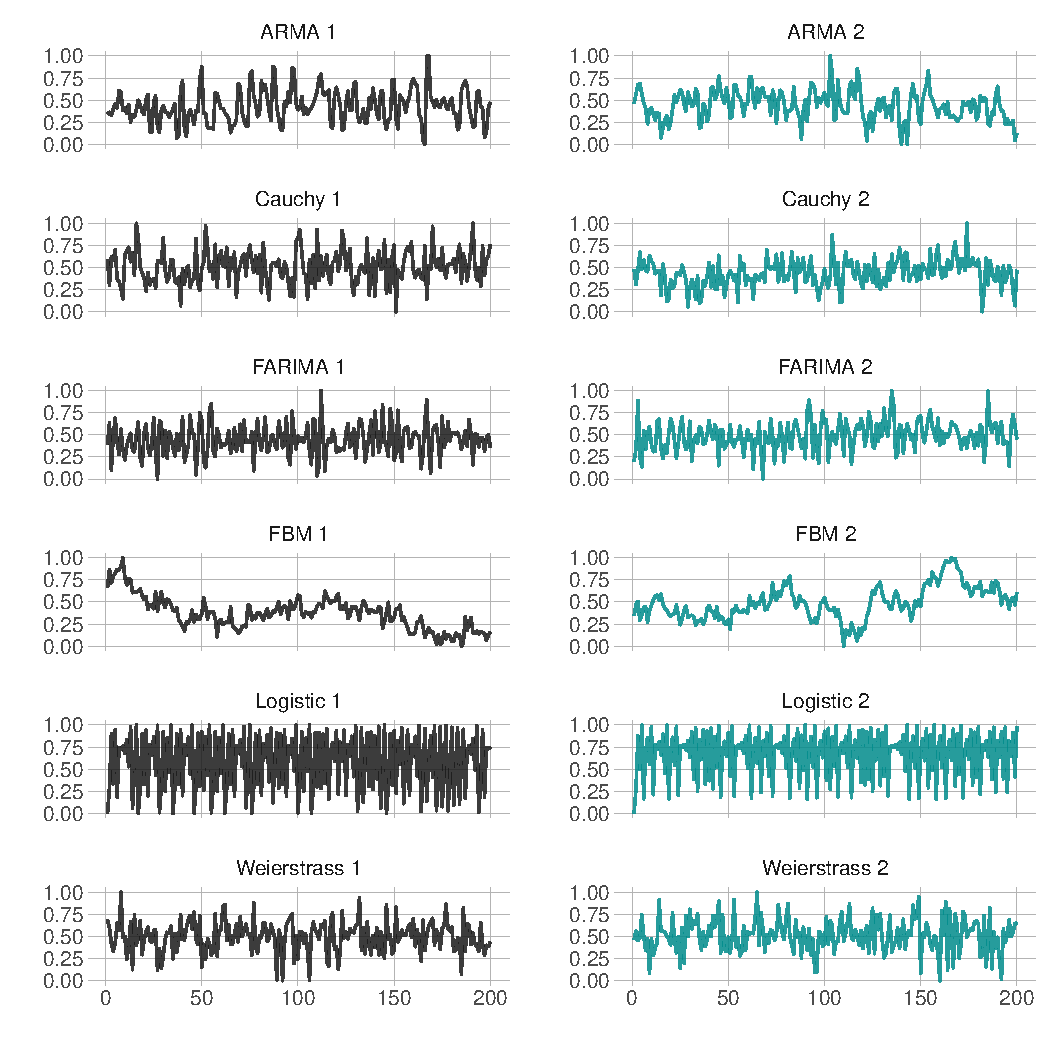
\includegraphics[width = \textwidth, keepaspectratio]{./figs/sim_jitter_plot_jitter_timeseries.pdf}
  % \end{picture}
  \end{center} 
  \caption{Sample functions from each simulation group.  }
   \label{fig:jitter-ts}
\end{figure}

\begin{figure}[!htbp]
  \begin{center}
  % \begin{picture}(60,60)
  % ./figs/coeff-interp-simple-functions1.pdf
  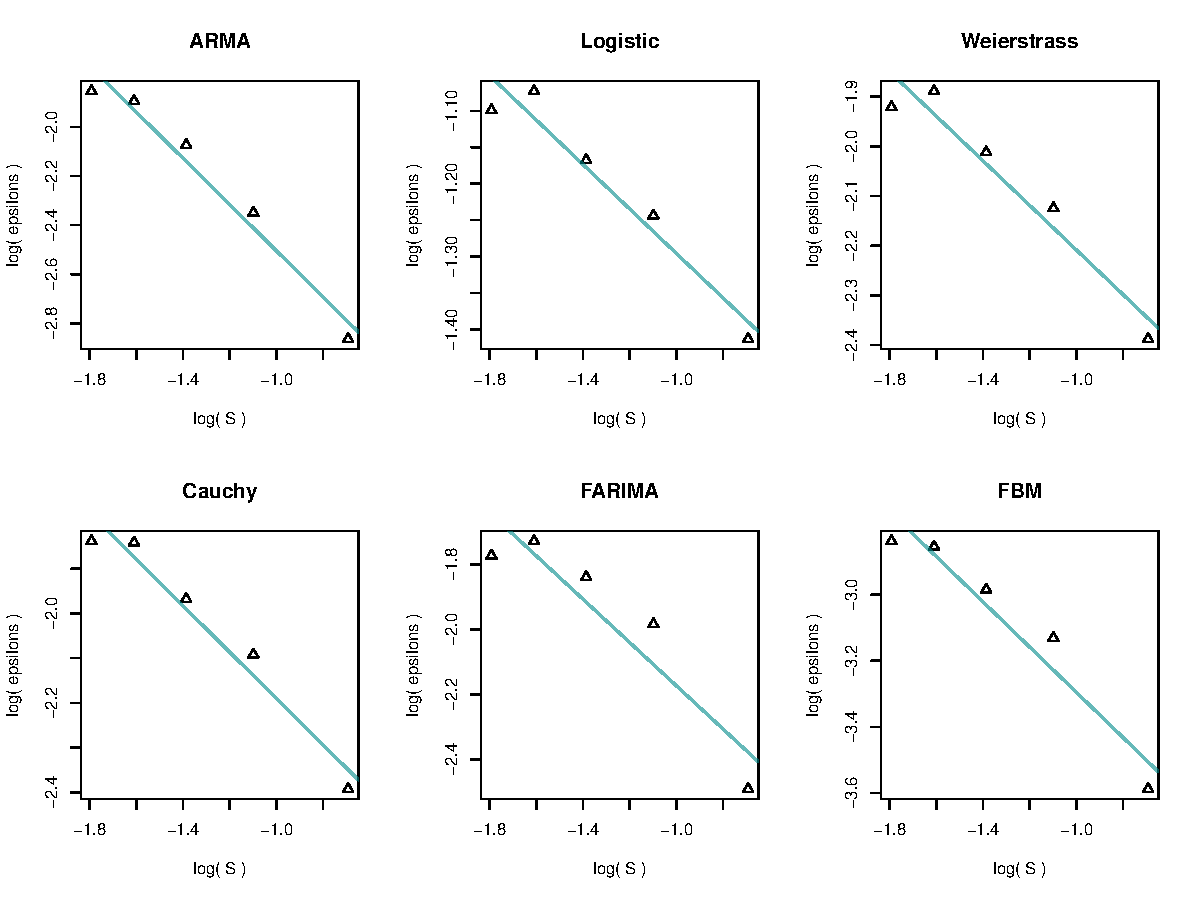
\includegraphics[width = \textwidth, keepaspectratio]{./figs/sim_jitter_plot-sim-fits.pdf}
  % \end{picture}
  \end{center} 
  \caption{Linear regression plots for the lifting scheme.}
  \label{fig:lift-lm}
\end{figure}

A plot of the complexity coefficients generated by each approximation method and group is shown in Figure \ref{fig:feature-space}. Each point represents where an individual function lies in the feature space of the two complexity coefficients $A$ and $B$. The coefficient values have been normalized to the $[0,1]$ interval so the plots show the relative distribution of the functions in the feature space.
Although we will quantify 
the ability of the approximation methods to 
separate the two simulation groups below, the scatter plot shows that the approximation methods place each process at similar coordinates in the 
complexity coefficient space. The scatter plots also show 
that some methods separated particular processes better. 
For example, the cubic spline method separates the two groups 
generated by ARMA(2,2) processes, as seen on the middle left-hand side of Figure \ref{fig:feature-space}.


\begin{figure}[!htbp]
  \begin{center}
  % \begin{picture}(60,60)
  % ./figs/coeff-interp-simple-functions1.pdf
  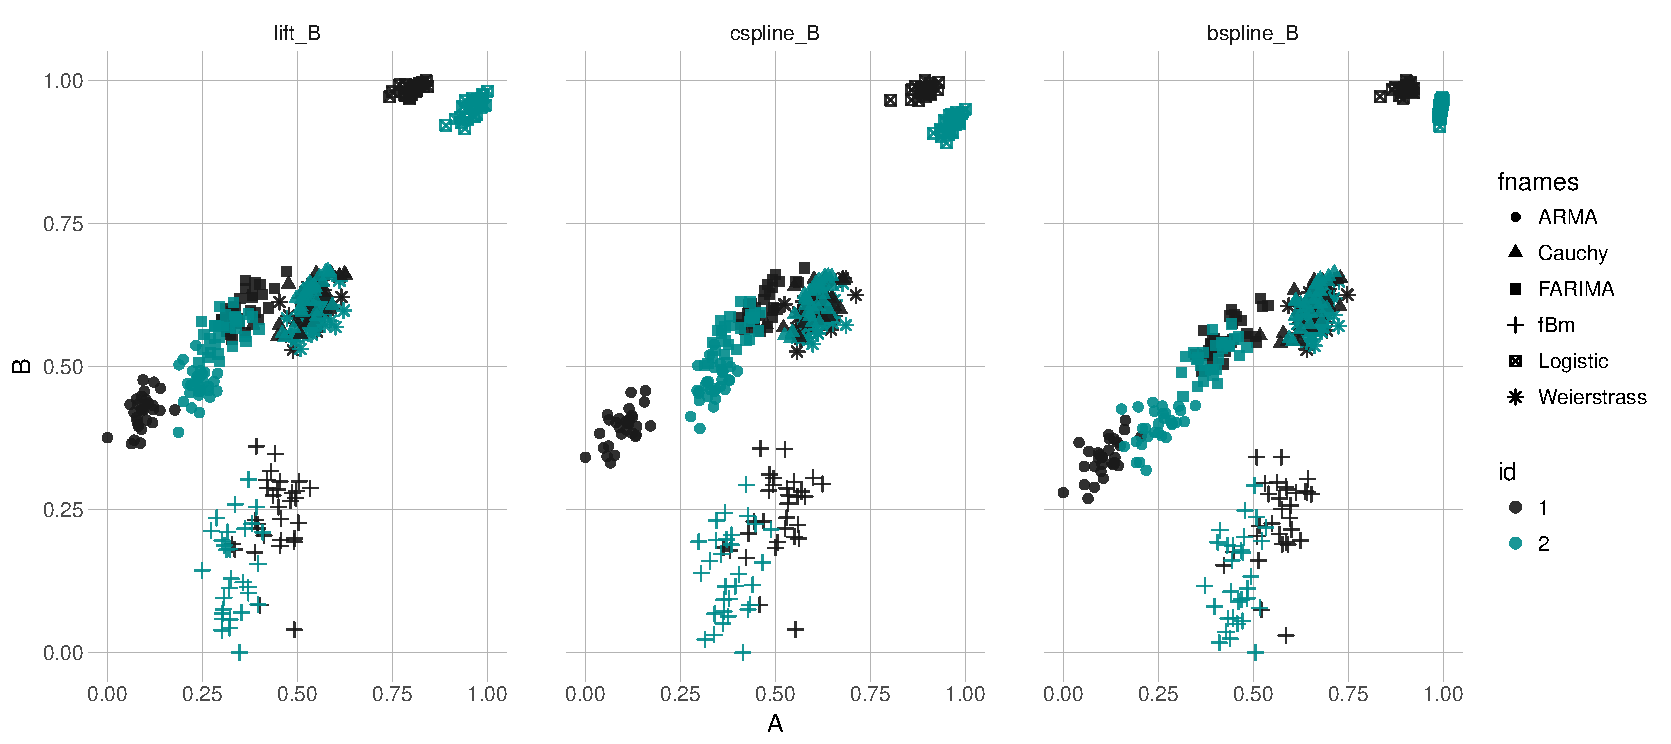
\includegraphics[width = \textwidth, keepaspectratio]{./figs/ecomplex_approx-feature-space.pdf}
  % \end{picture}
  \end{center}
  \caption{The two simulation groups plotted in the 
  complexity coefficient space.}
  \label{fig:feature-space} 
\end{figure}


The scatter plot of the simulations also provides some information 
about the direction in which the simulations are separable. If the 
simulations from each group were separable along a single axis, 
either vertically or horizontally, this would indicate that a single
complexity coefficient could be used to separate the groups.
 % In the following chapter, we compare how the complexity coefficients and fractal dimension vary with the parameters several functions. Based on those tests it is unclear whether the intercept coefficient $A$ adds contributes information that can be used in discriminating two functions that are not found in slope coefficient $B$.
 % and the variogram estimator of fractal dimension were reflected changes in the parameters controlling the H\"older class of the function. 
 % Except in the case of the random phase Weierstrass function, the intercept coefficient $A$ seemed to follow a similar pattern as the slope coefficient. 
 Figure \ref{fig:feature-space} shows that for the processes that are readily separable \textemdash fBm and the ARMA and logistic simulations \textemdash both the slope and intercept coefficient appear to be useful in separating the two sets of simulations. For example, both the fBm and ARMA simulations are well separated along the $x$-axis, corresponding
 to the complexity coefficient $A$. On the other hand, the realizations of the logistic map in the upper right hand corner appears separable on the diagonal meaning both complexity coefficients contributed to differentiating the two simulation groups.

Using the first set of simulations described above, 30 samples were 
generated and a total approximation error for each method was calculated. 
The approximation error was calculated by 
taking a simple sum of errors at each down sampling level $h$: 
\[
  \varepsilon_{\mathcal{F}} = \sum_{h} \varepsilon_{h, \mathcal{F}}.
\]
Table \ref{tab:epsilons-all} shows the mean approximation error 
over the 30 samples.
The B-spline method had the lowest MSE for all processes.
Since the B-spline method produced the minimum 
error for each function, the combined method 
simply reflects that of the B-spline approximation.
The lifting method produced a slightly lower mean error but 
the cubic spline and lifting errors are very similar for each
simulation. 

\begin{table}[!htbp] \centering 
\begin{tabular}{@{\extracolsep{1pt}} ccccccc} 
\\[-1.8ex]\hline 
\hline \\[-1.8ex] 
  Function & Lift & Cspline & Bspline & Combined \\ \hline 
ARMA       & 0.10  & 0.11    & 0.07 & 0.07 \\ 
Cauchy       & 0.09  & 0.10  & 0.06 & 0.06 \\ 
FARIMA       & 0.13  & 0.14  & 0.08 & 0.08 \\ 
fBm          & 0.03  & 0.04  & 0.02 & 0.02 \\ 
Logistic     & 0.30  & 0.32  & 0.20 & 0.20 \\ 
Weierstrass  & 0.14  & 0.15  & 0.09 & 0.09 \\ 
\hline \\[-1.8ex] 
          \end{tabular} 
  \caption{Mean total approximation error for 30 samples of each simulation. 
             }
  \label{tab:epsilons-all}
\end{table}


\begin{table}[!htbp] \centering 
\begin{tabular}{@{\extracolsep{1pt}} ccccccc} 
\\[-1.8ex]\hline 
\hline \\[-1.8ex] 
Function    &  Lift & Cspline & Bpsline  & Combined 
                                       \\ \hline
ARMA        & 0.03 &   0.00 &   0.07 &   0.07  \\ 
Cauchy      & 0.65 &   0.53 &   0.52  &    0.53  \\ 
FARIMA      & 0.32 &   0.30 &   0.32  &    0.33 \\ 
fBm         & 0.20  &   0.22  & 0.20 &  0.22  \\ 
Logistic    & 0.00 &   0.00 &   0.00  &    0.02  \\ 
Weierstrass & 0.50 &   0.43 &   0.45  &    0.45  \\
\hline \\[-1.8ex] 
          \end{tabular} 
  \caption{Classification errors using complexity coefficients  
  $A$ and $B$ for each approximation method.}
  \label{tab:error-all}
\end{table}

The set of complexity coefficients as computed by each 
approximation method were then used to classify the 30 samples from each simulations. The classifier was a random forest with 
500 trees with 3 features used to determine branches. The overall out-of-bag classification error is reported in Table \ref{tab:error-all}. The cubic 
spline method performed equally well or better
on 4 of the 6 methods, but the results of all methods are 
similar.

% Finally we tested whether the classification error varied with the loss function used to compute approximation error. Again, accuracy computed as the out-of-bag classification accuracy of a random forest classifier. Both the mean squared error, mean absolute error(MAE) loss function performed similarly with MAE performing slightly better. 

% \begin{table}[!htbp] \centering 
% \begin{tabular}{@{\extracolsep{1pt}} ccccccc} 
% \\[-1.8ex]\hline 
% \hline \\[-1.8ex] 
% Function     &   MAE  &  MSE   & Max \\
% ARMA         &   0.00  &  0.03  & 0.33 \\ 
% Cauchy       &   0.52  &  0.66  & 0.47 \\ 
% FARIMA       &   0.18  &  0.22  & 0.39 \\ 
% fBm          &   0.13  &  0.16  & 0.33 \\ 
% Logistic     &   0.01  &  0.00  & 0.18 \\ 
% Weierstrass  &   0.44  &  0.53  & 0.51 \\
% \hline \\[-1.8ex] 
%           \end{tabular}  
%   \caption{Classification error using a random forest clasysifier 
%            and three different loss functions.}
%   \label{tab:error-mse}
% \end{table}
 
\section{Computational Efficiency}

 For our set of processes, classification performance did not appear adversely affected by the slightly lower approximation accuracy of the lifting and cubic spline methods. However, both the cubic spline and lifting approximation methods are computationally more efficient than the B-spline method. Both methods are linear in the number of inputs and both are linear or constant in terms of their space complexity, that is, 
the amount of memory needed to store intermediate computations is linear or constant function of the size of the inputs. 

The execution time of each approximation method was estimated
using the system time taken to complete approximations on 
inputs of size $10^7$ to $10^{13}$. 
The average computational time for
each input size on a log scale is shown in Figure \ref{fig:benchmark}.
For our implementation, 
the B-spline method increases the number of knots linearly with 
the inputs and the associated design matrix grows quadratically
with the number of inputs. This leads to the B-spline method becoming 
infeasible for even moderately large inputs. 
Although the cubic spline and lifting method are computationally 
linear, the lifting scheme was implemented entirely in the \texttt{R}
language. The cubic spline method is called from \texttt{R} but 
most calculations are calculated in the more computationally efficient \texttt{C} language. Although it is not clear in Figure 
\ref{fig:benchmark}, the cubic spline method was an order of magnitude faster than the lifting scheme. 

\begin{figure}[!htbp]
  \begin{center}
  % \begin{picture}(60,60)
  % ./figs/coeff-interp-simple-functions1.pdf
  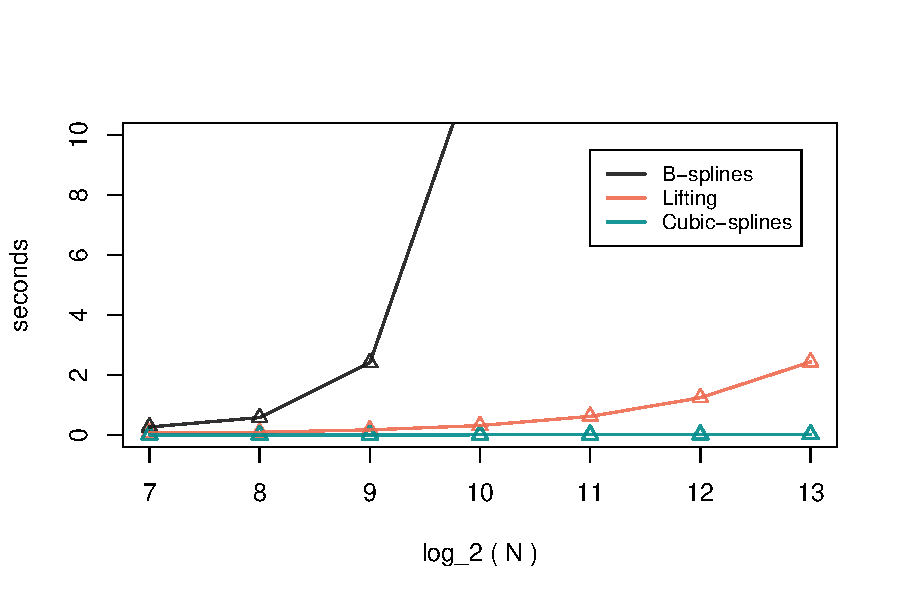
\includegraphics[width = \textwidth, keepaspectratio]{./figs/benchmark-benchmark.pdf}
  % \end{picture} 
  \end{center}
  \caption{Computational time of each approximatino method
   as a function of the size of the log of the input.}
  \label{fig:benchmark} 
\end{figure}

% Since both complexity coefficients were useful 
% in discriminating between functions drawn from similar sets of parameters, we also used both coefficients to 

Our primary goal of the preceding test was to determine 
if enlarging the set of approximations would lead to improved 
performance of the complexity coefficients. We assumed 
that the enlarged set would allow for improved approximation error 
and a better estimation of the complexity coefficients. 
Here we measured 
performance by the ability of the complexity coefficients to 
discriminate between closely related simulations. Lower 
approximation errors did not correspond to better classification
accuracy, however. The cubic spline method was the most computationally efficient and performed as well or better on the classification test as the other methods. Based on these results,
the cubic spline approximation was used for the applied work in 
Chapters 4 and 5.






 
\chapter{H\"older Conjecture} 
% 
% The complexity coefficients were designed, as their name implies, to capture the complexity of a times series. 

In this chapter, we explore how the complexity coefficients relate to other characteristics of time series. In particular, we use a number of simulations to examine the relationship between the complexity coefficients and both the H\"older class of a function and the fractal dimension of the function's graph. We begin by looking the behavior of
the complexity coefficients for a few simple functions with added noise. The complexity coefficients are given by parameters of $\log-\log$ linear fit to points whose original values is less than 1 and the interpretation of the parameters may not be intuitive. These simple examples are meant to orient the reader in interpreting some aspects of the complexity coefficients.  

% value of the complexity coefficients for a few 
% simple functions. 

\section{The Complexity Coefficients}
In the theoretical development of $\varepsilon-$complexity, 
the continuous function to be analyzed was assumed to on 
the interval $[0,1]$. Here we refer instead to the index
of the samples of the function which, like the time 
parameter of a time series, are in $\{ 1,2,3,.... \}$.
The complexity coefficients are computed by finding the best approximation to a function as that function is downsampled by integer amounts, that is, points indexed by $h\N$ are used in the reconstruction. In our implementation of the algorithm, a function is downsampled at $h \in \{ 2,3,4,5,6 \}$ giving us 
five downsampling levels. The minimal approximation error, $\varepsilon_h$ is computed for each level $h$. We denote the  proportion of the samples retained $\mathbb{S}_h = \frac{1}{h}$.
The $\varepsilon-$complexity coefficients $A, B$ are then result of an ordinary least squares fit: 
\[
     \log(\varepsilon_h) = A + B \mathbb{S_h}.
\]


\begin{figure}[h]
  \begin{subfigure}[b]{0.45\textwidth}
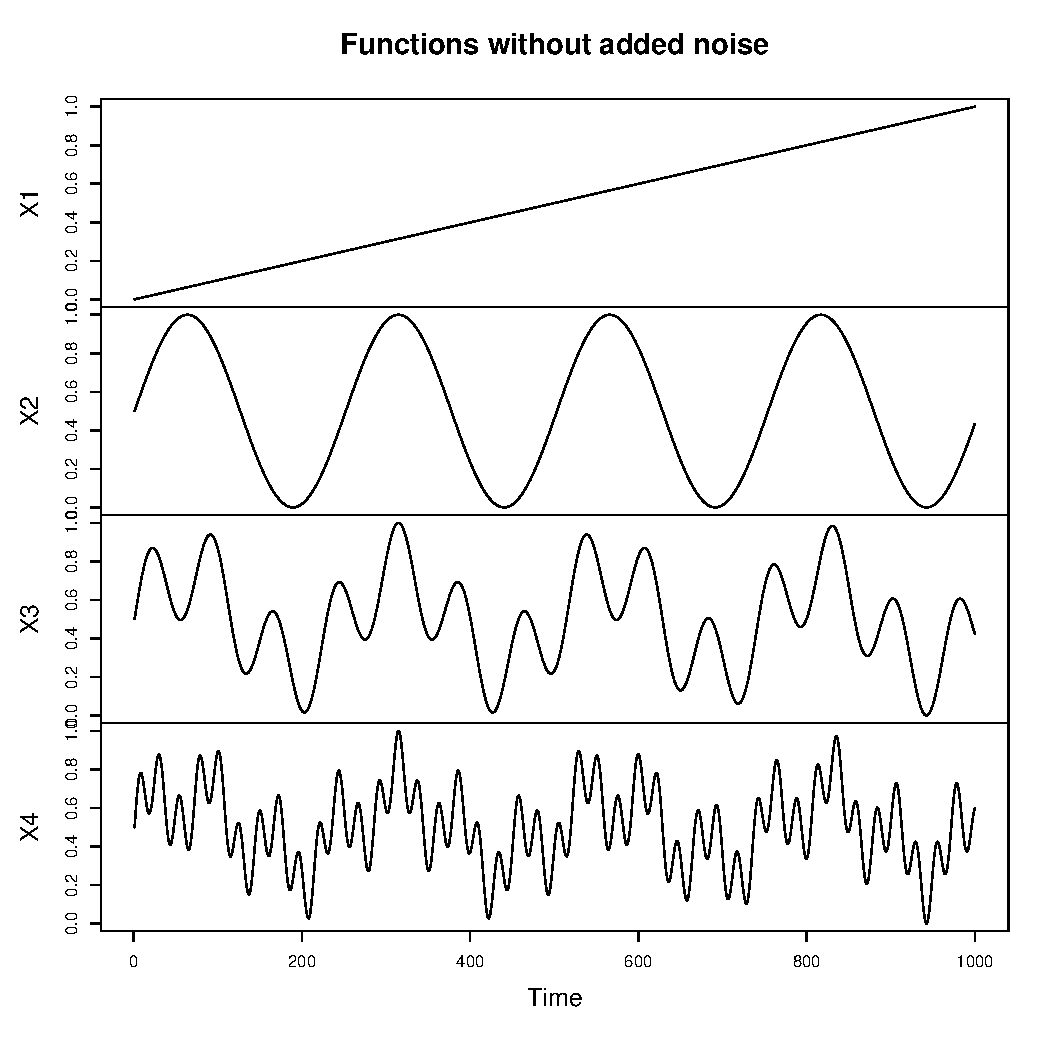
\includegraphics[width = 0.9\linewidth, height = 3in]{./figs/coeff-interp-simple-functions0.pdf}
    % \caption{Functions without added noise.}
    % \label{fig:simple-functions1}
  \end{subfigure}
  \hfill
  \begin{subfigure}[b]{0.45\textwidth}
  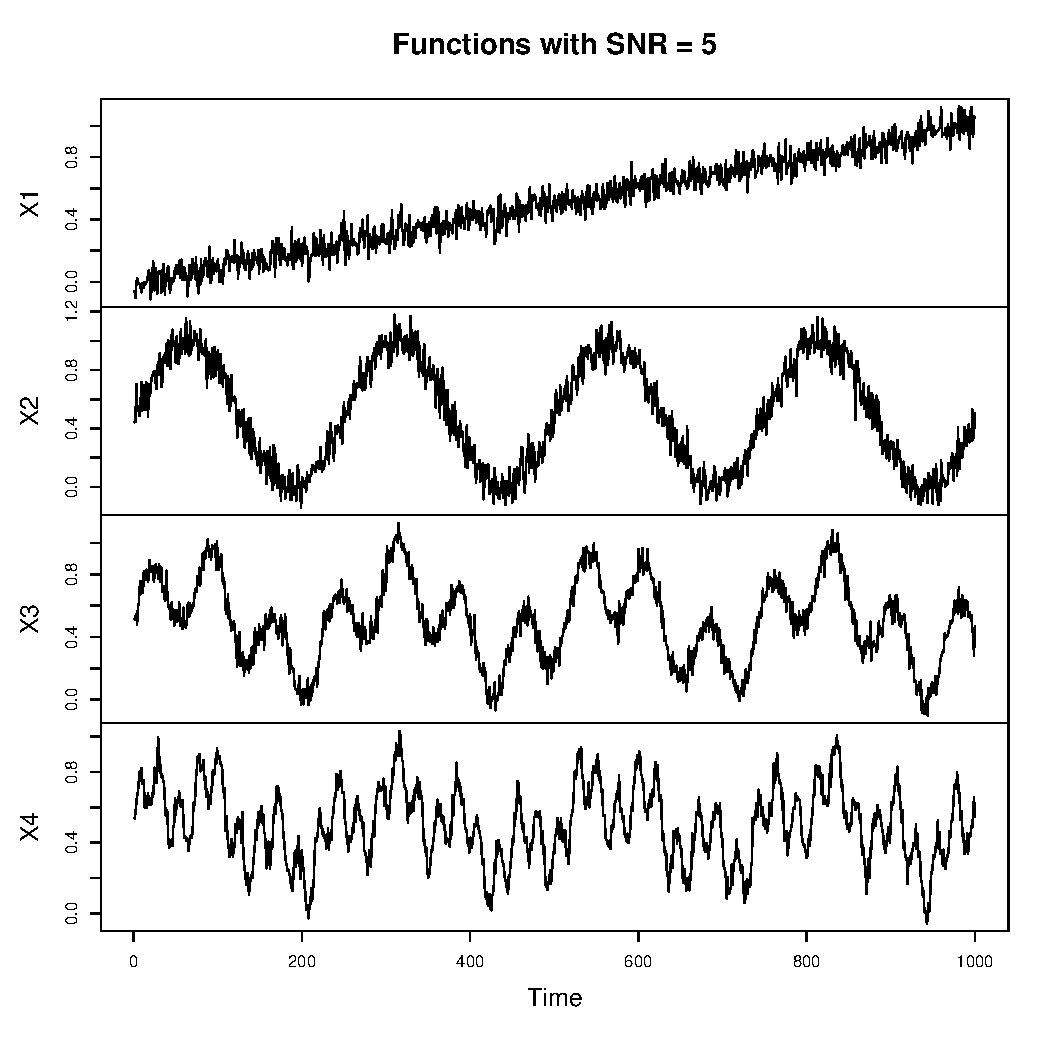
\includegraphics[width = 0.9\linewidth, height = 3in]{./figs/coeff-interp-simple-functions1.pdf}
  % 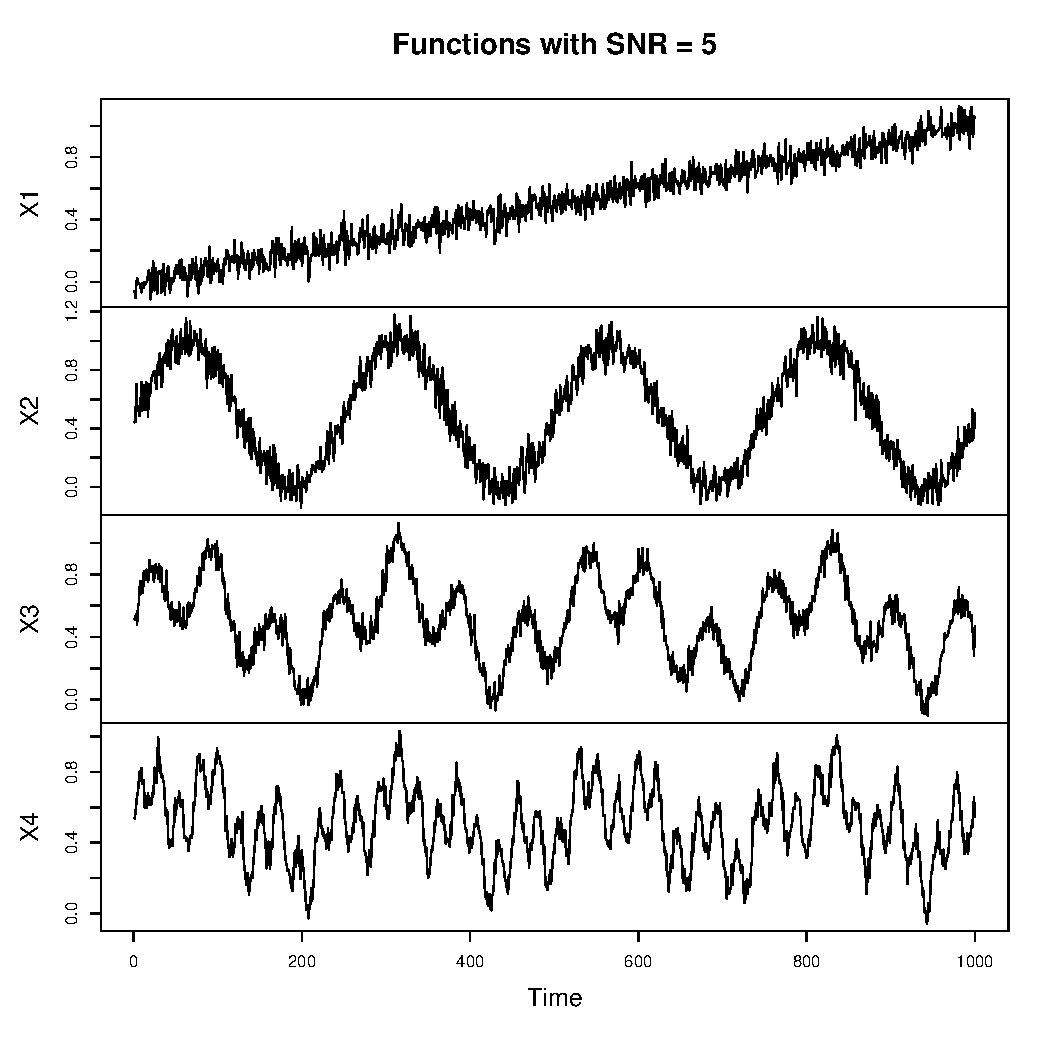
\includegraphics[width = 0.9\linewidth, height = 3in]{./figs/coeff-interp-simple-functions1.pdf}
    % \caption{Functions without added noise.}
  \end{subfigure}
  \caption{Simple linear and sinusoidal functions with and 
  without added noise.}
     \label{fig:simple-functions}
\end{figure}

  \begin{figure}[h]
    \begin{center}
    % \begin{picture}(60,60)
    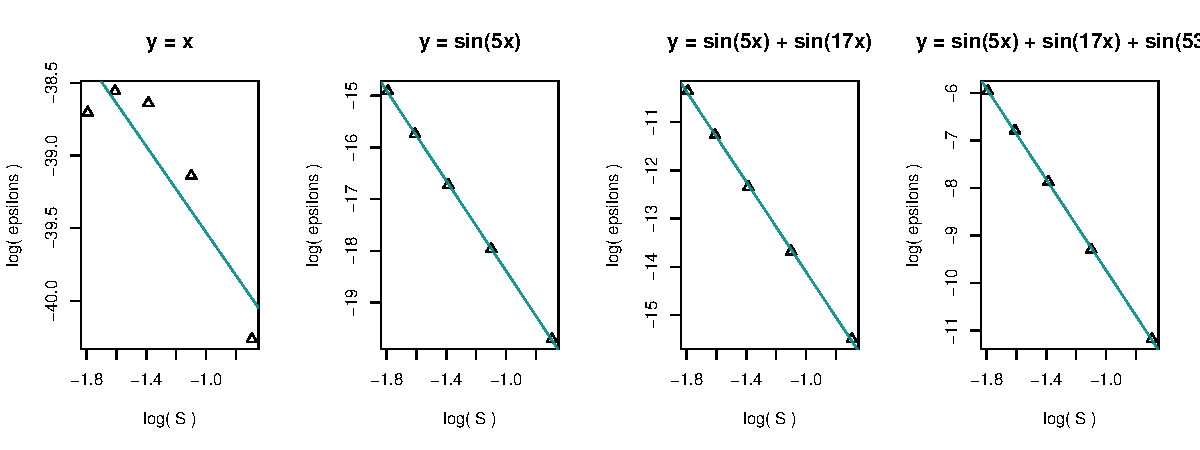
\includegraphics[width = \textwidth, keepaspectratio]
    {./figs/coeff-interp-simple-fits.pdf}
    % \end{picture}
    \end{center}
    \caption{The log-log linear fit of the approximation errors 
    against the proprotion of points $\mathbb{S}_h$ used to 
    approximate the functions \ref{fig:simple-functions}}.
    \label{fig:simple-fits}
  \end{figure}

% \begin{figure}[!htbp]
%   \begin{center}
%   % \begin{picture}(60,60)
%   \includegraphics[totalheight = 3.4in]
%   {./figs/coeff-interp-simple-functions0.pdf}
%   % \end{picture}
% \end{center}
% \end{figure}
% \begin{figure}[!htbp]
%   \begin{center}
%   % \begin{picture}(60,60)
%   \includegraphics[totalheight = 3.4in]
%   {./figs/coeff-interp-simple-functions1.pdf}
%   % \end{picture}
% \end{center}
% \end{figure}

% (fig: simple-functions)

Figure \ref{fig:simple-functions} shows a linear function and 
three sinusoidal functions. Figure \ref{fig:simple-fits} 
shows the $log-log$ regression of the errors $\varepsilon_h$ 
on the fraction of samples kept $\mathbb{S}_h$. The complexity coefficients for these fits are given in Table \ref{tab:simple-coeffs}. While these simple functions will not reveal much about the behavior of the complexity coefficients for more complicated time series, the results highlight some basic properties of the complexity coefficients.  

\begin{table}[!htbp] \centering 
\begin{tabular}{@{\extracolsep{1pt}} ccccccc} 
\\[-1.8ex]\hline 
\hline \\[-1.8ex] 
Without Noise     &  $A$ & $B$  & $\hat D$ \\ \hline 
        $x $    &    -41.45 & -1.92  & 1.000\\ 
 $\sin 5x$  &
                  -22.71 & -4.33 & 1.001 \\ 
 $\sin 5x  + \sin 17x$ &
                  -18.71 & -4.61 & 1.001 \\ 
 $\sin 5x  + \sin 17x + \sin 53x $ &
                  -14.54 & -4.81 & 1.010 
 \\ \hline  
% \hline \\[-1.8ex] 
                 % \end{tabular} 
% \begin{table}[h]
% \begin{center}
%   \begin{tabular}{ | c | c |  c| c| } 
%    
SNR = 20  & $A$ & $B$ & $\hat D$ \\  \hline
$x  $ &
   -4.04  & -0.57   &  1.97 \\  
 $\sin 5x   $ &  
   -3.9  & -0.59   &  1.94 \\  
 $\sin 5x  + \sin 17x  $ &
   -4.07  & -0.55   &  1.94 \\  
$\sin 5x  + \sin 17x + \sin 53x $ & 
   -4.12  & -0.52   &  1.67 
\\ \hline 
SNR = 5    & $A$ & $B$& $\hat D$  \\ \hline
$ x$ &
 -3.39 & -0.54   &  1.99  \\ 
 $\sin 5x $ &
 -3.48 & -0.55   &  1.99  \\ 
 $\sin 5x  + \sin 17x $ &
 -3.58 & -0.55   &  1.99  \\ 
 $\sin 5x  + \sin 17x + \sin 53x $ &
 -3.70 & -0.58   &  1.82  \\
 \hline \\[-1.8ex] 
    \end{tabular}
  \caption{Complexity coefficients and fractal dimension, $\hat D$,
  estimates for a linear and several sinusoidal functions.}\label{tab:simple-coeffs}  
\end{table}

The linear fits in \ref{fig:simple-fits} determine the complexity 
coefficients $A,B$. The $x-$axis is the log of the  $\mathbb{S}_h$, percent of points used to approximate the original function at each step. The finest scale approximation is when $h=2$, represented by the point with the least (log) error located furthest to the right at $log( S )\approx -0.7$. Small values for this error correspond to accurate approximations and less variability at the finest scale of the sampled function. 
In theory, the approximation error at zero represents the exact approximation of the function. Since we are computing the log of the approximation error $\varepsilon$, as 
$\varepsilon \to 0, \log(\varepsilon) \to -\infty$. For 
the three simple functions in Figure \ref{fig:simple-functions}
the overall approximation error is low, and at least for these
examples the intercept value $A$ decreases with simpler 
functions.

The slope coefficient $B$ should measure the rate at which the approximation error grows as fewer points are used to approximate the original function. The coefficient for the sinusoidal functions is fairly similar at each noise level. The relation between 
the value $B$ and the number of frequency components in the functions is not clear as the order $B$ for these functions 
changes with added noise.

 % The coefficient should indicate the rate of change in the approximation error as we go from coarser to finer scales, or from left to right on \ref{fig:simple-fits}.



% Figure \ref{fig:simple-functions} shows the functions with 
% added noise. 
% The complexity coefficients 
% computed on a single example of each function with 1000 
% points taken on the interval $[0,5]$. The intercept increases as the noise to signal ratio is increased. 
% It is not obvious how to interpret the change in the slope coefficient $B$. For the set with  
% more noise, the functions with higher frequency sinusoidal components have a steeper slope, whereas the simpler functions generally have a less steep slope as more noise is added.  

The fractal dimension reported in Table \ref{tab:simple-coeffs}
is estimated using a variogram method described in Chapter 2. Below we compare the variogram estimate of the fractal dimension of for a number of functions to the complexity coefficients. 
Here we point out that increasing noise dramatically 
affects the fractal 
% $\mathop{E}(X_t)  = \mu_{t}$ 
dimension estimate $\hat D$. This fractal dimension estimator sets the maximum estimate of a function whose graph is in $\R^2$ to the theoretical maximum of 2. Adding a small amount of noise makes the estimator approach its maximum quickly.


\section{H\"older Class and Fractal Dimension}

Theorem \ref{thm:holder} states a relationship 
between a H\"older class of functions 
and the complexity coefficients. The proof of the theorem differs in some details from the method of estimating the complexity coefficients. 
For example, the proof assumes the error is 
achieved by taking the infimum over a possibly 
infinite family of functions $\mathcal{F}$,  
and the max norm rather than the Euclidean 
norm. In addition, the statement relates
the $\varepsilon-$complexity to a class 
H\"older continuous functions, although the 
same relation should hold for individual members
of that H\"older class.
In this section, we use several functions that 
have a known H\"older exponent and that 
have parameters that can modulate the 
H\"older exponent of the function. We use these functions to test the conjecture that the H\"older class of a function can be characterized
by its the complexity coefficients.  

In Chapter 2 we reviewed some relationships between 
the H\"older exponent and 
to the fractal dimension of a function. For example,
for a bounded continuous function $f:\R \to \R$, 
satisfying the H\"older condition 
\[
  |f(t) - f(t+h)| \leq c|h|^{\alpha}
\]
the box counting dimension $\dim_B(f)$ is bounded above
by $2- \alpha$\cite{falconer2003}. 
% We use the variogram estimator 
% that is the slope of a least-squares fit to 
% the log-log plot of the variogram $\gamma(h)$, 
% \[
% \gamma(h) = \frac{1}{2}\mathbb{E}\left(X_t - X_{t + h} \right)^2.
% \]
% against the time increments $h$.
Our experiments show a close relationship between the variogram 
estimator of fractal dimension $\hat D$ and the slope parameter of the complexity coefficients $B$. 
For the functions or sample paths of stochastic processes
 used in our tests there is a linear relationship 
 between the H\"older class of the function 
 and the functions fractal dimension. If 
 the complexity coefficients and the slope 
 parameter $B$ identify the H\"older class then 
 for these functions, they should identify the 
 fractal dimension of the graphs as well.
 There is also an 
 intuitive relationship between the 
 variogram estimator of fractal dimension and 
 the method of computing $\varepsilon-$complexity 
 coefficients; for a given increment $h$, the 
  variogram estimator uses the expected value 
  of the square the increments, 
   $E[(X_t - X_{t + h})^2]$, while the complexity
   cofficients finds the approximation error 
   over all intervals $h$. A larger approximation 
   error on increments $h$ likely corresponds 
   with greater expected difference $X_t - X_{t +h}$
   and vice-versa. 

% The variogram at values $h$ is the expected value 
% of the increment 
% \[
%   \mathbb{E}\left(X_t - X_{t + h} \right)
% \]
% while $\varepsilon$-complexity calculates the 
%  approximation error
% \[
%    \epsilon_h   = | \hat x(t) - x(t)| 
% \]
% for each increment $h \in \{ 2,3,4,5,6 \}$. 
% Here we examine how the
% complexity coefficients $A, B$ change as 
% we manipulate the parameters of several 
% functions that control the H\"older class 
% or fractal dimension of the functions. 

For the following tests, we generated samples of between 
500 and 2000 for each of four functions, the Weierstrass
and random phase Weierstrass functions, fractional 
Brownian motion(FBM) and the Cauchy process. The first three have a single parameter $\alpha$ which 
controls both the H\"older exponent and fractal 
the dimension of each while the Cauchy process has two parameters 
which separately control the fractal dimension and 
long-range dependence of the function. 

\begin{figure}[h]
  \begin{subfigure}[b]{0.49\textwidth}
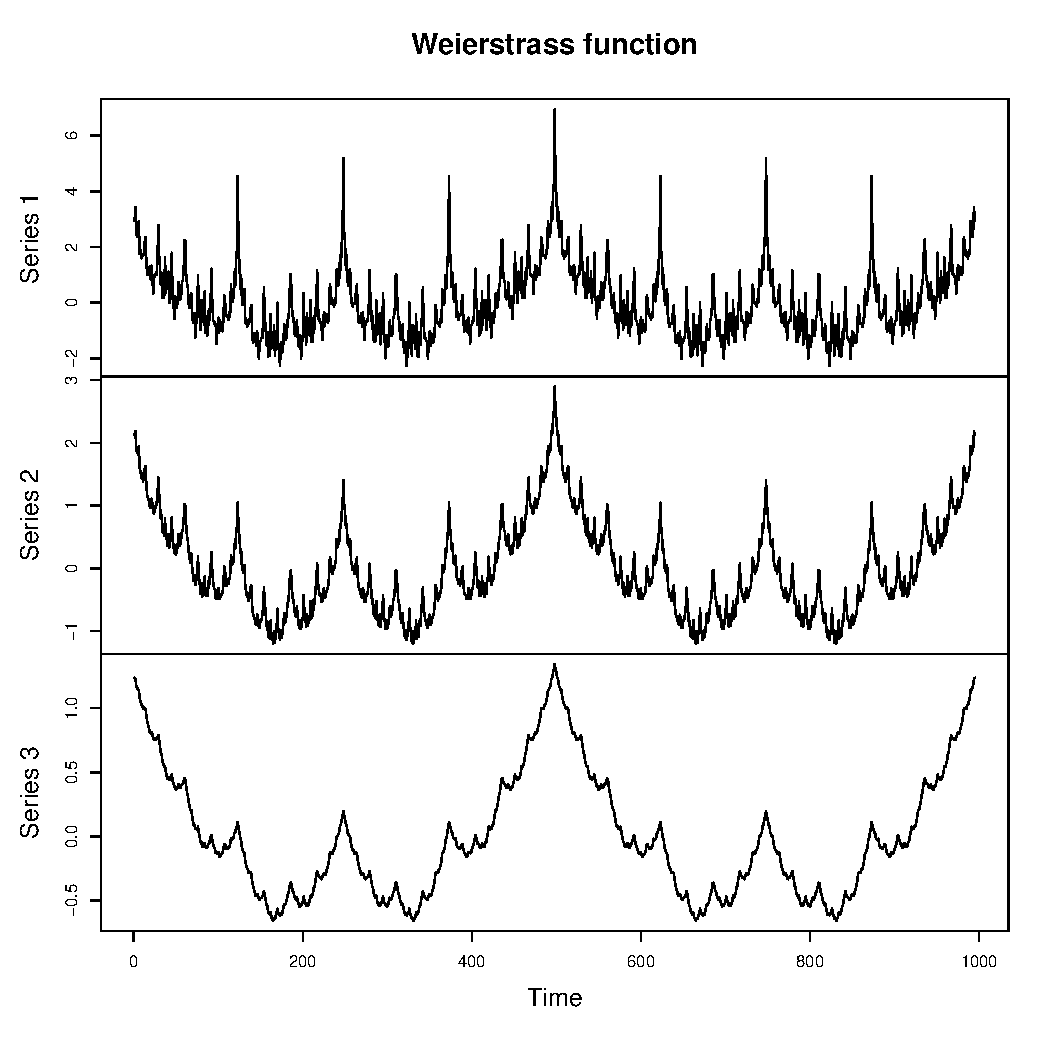
\includegraphics[width = 0.9\linewidth, height = 3in]{./figs/holder_notrandom-weier-notrandom.pdf}
    % \caption{Functions without added noise.}
    \label{fig:weierstrass}
  \end{subfigure}
  \hfill
  \begin{subfigure}[b]{0.49\textwidth}
  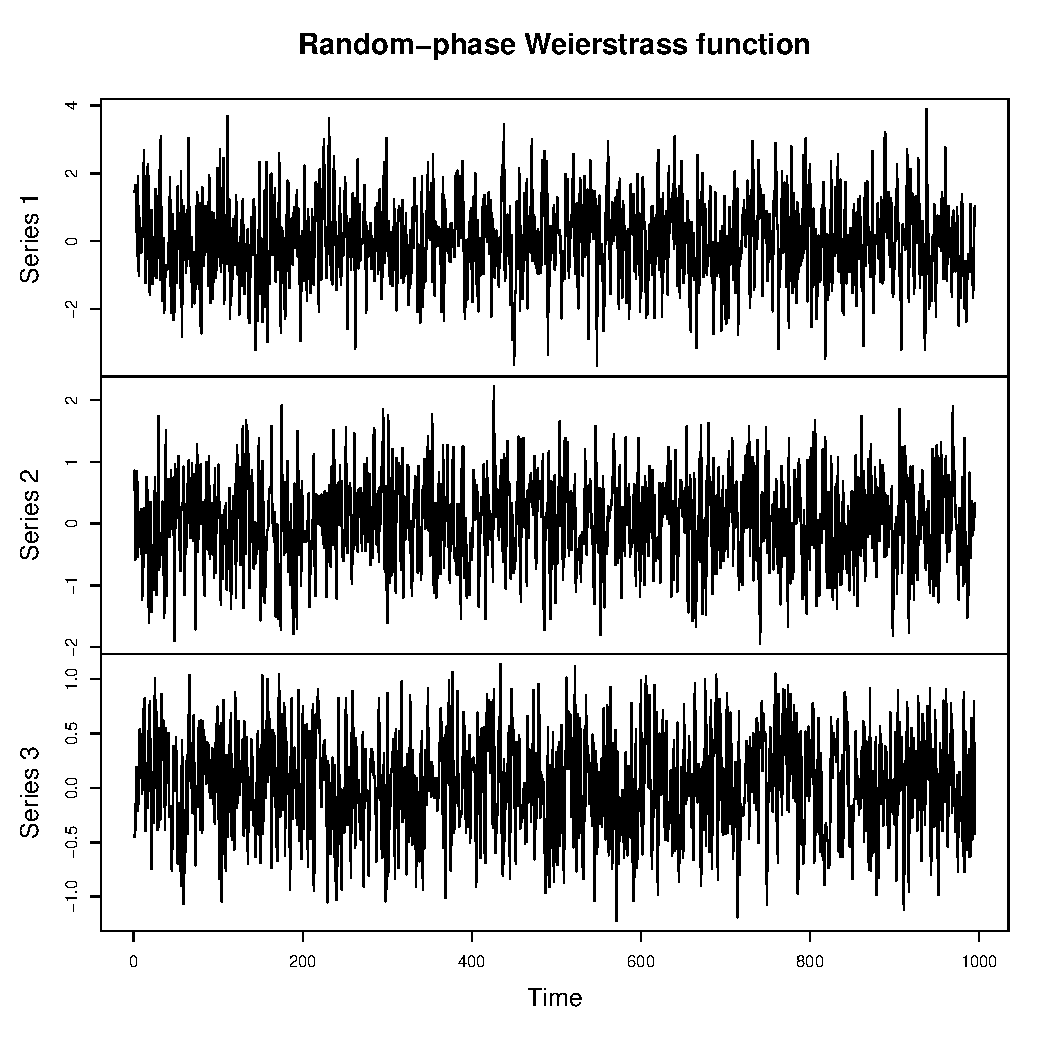
\includegraphics[width = 0.9\linewidth, height = 3in]{./figs/holder_coeffs-weier-random.pdf}
    % \caption{Functions without added noise.}
  \end{subfigure}
  \caption{The Weierstrass and random-phase Weierstrass function
  for $\alpha = \{ 0.20, 0.42, 0.80 \}$}
    \label{fig:weierstrass}
\end{figure}

\begin{figure}[!htbp]
  \begin{center}
  % \begin{picture}(60,60)
  % ./figs/coeff-interp-simple-functions1.pdf
  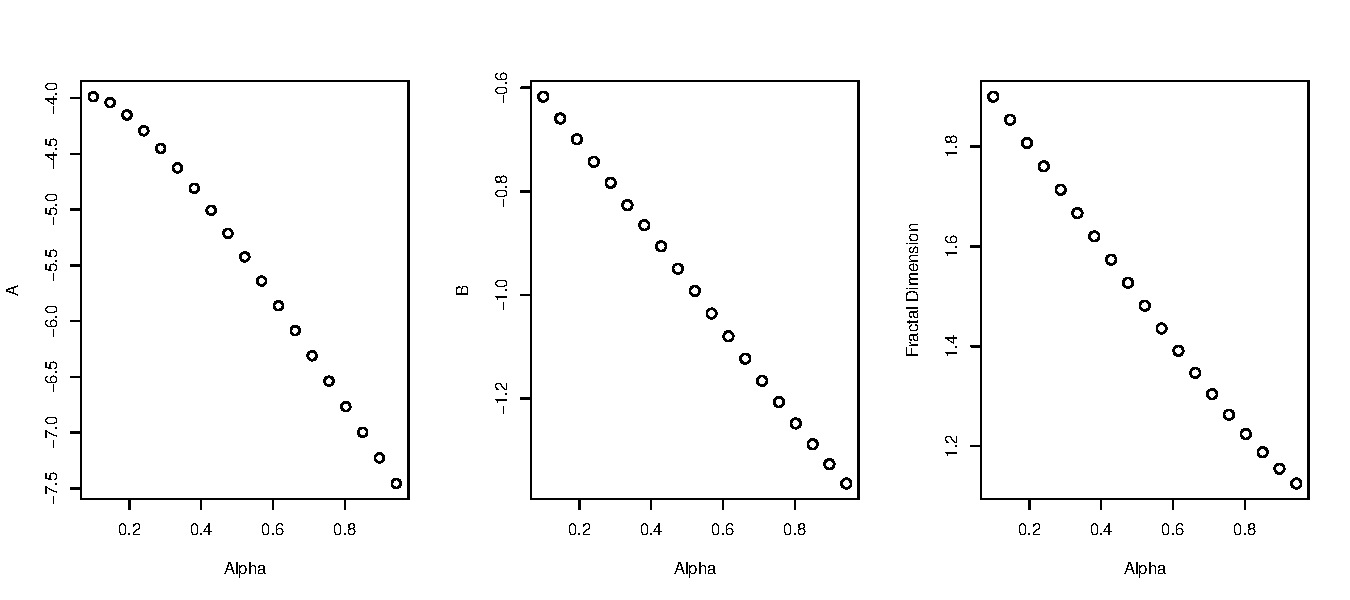
\includegraphics[width = \textwidth, keepaspectratio]{./figs/holder_notrandom-param-plots-notrandom}
  % \end{picture}
  \end{center} 
  \caption{Complexity coefficients and fractal dimension 
  plotted against the Weierstrass functions $\alpha$ parameter.  }
  \label{fig:notrandom-params}
\end{figure}


% \begin{figure}[!htbp]
%   \begin{center}
%   % \begin{picture}(60,60)
%   \includegraphics[height = 10cm,width = 10cm, keepaspectratio]
%   {./figs/holder_notrandom-fd-vs-B.pdf}
%   % \end{picture}
%   \end{center}
%   \caption{The complexity coefficients $B$ of the Weierstrass 
%   function 
%   plotted against the variogram estimate of fractal dimension.}
%   \label{fig:notrandom-B-fd} 
% \end{figure}

The  Weierstrass function written
\[
  W_{\alpha}(x) 
  \hspace{1em}= \sum_{n = 0}^{\infty} b^{-n \alpha} \cos(b^n \pi x).
\]
is H\"older $\alpha$ for $0 < \alpha < 1$ and has box-counting dimension $D-\alpha$.  
% The parameter $\alpha$ of the Weierstrass function 
% anhe 
% H\"older class and fractal dimension of the functions --  
% box-counting dimension for the deterministic 
For the random-phase Weierstrass function, as proved by Hunt\cite{hunt1998}, 
the parameter $\alpha$ determines the Hausdorff dimension of its graph. 
The two functions are illustrated in Figure \ref{fig:weierstrass} 
for three different paramaeter values $
\alpha = \{ 0.20, 0.42, 0.80 \}$. 
For smaller $\alpha$ the fractal dimension $D$ of the 
graphs increase.

Figure \ref{fig:notrandom-params} shows the change
in the complexity coefficients $A$ and $B$ and the
variogram fractal estimator $\hat D$ as the parameter 
$\alpha$ is varied. The relation of both the 
complexity coefficient $B$ and fractal estimator $\hat D$ to 
$\alpha$ is linear. For the complexity intercept 
$A$ there is some non-linear change for low values of $\alpha$. The fractal estimator 
$\hat D$ closely tracks the theoretical fractal. 

% Figure \ref{fig:notrandom-B-fd}
% shows that the complexity coefficient $B$ changes 
% linearly with the fractal estimator $\hat D$. 

The results for the Weierstrass function are deterministic, 
so the results shown are for a single estimate for 
each parameter.
The remaining functions are stochastic so the same 
the test was run on fifty samples functions or simulations the
estimated complexity coefficients and fractal dimension 
estimate are displayed as box plots to shown the distribution
of the estimates.

% ===============a=========================================
%  Holder, fBM and Cauchy section
% ========================================================
% holder_coeffs-weier-random.pdf
% alpha = 0.1936842 0.4278947 0.8026316
For the random-phase Weierstrass function Figure 
\ref{fig:rp-weierstrass-boxplot} shows there 
was no relationship between the change in the $\alpha$ 
parameter and the complexity coefficient $B$ or 
fractal estimator $\hat D$. The intercept coefficient $A$ increases 
linearly but the total magnitude of the change is 
relatively small-- the median of the estimates has a range 
of less than $0.5$. The 
reported results were for simulations of 2000 
points. The simulation was repeated at for lengths between 
500 and 2000 but the returned the same results. We 
do not have an explanation for the discrepancy between 
the theoretical H\"older class and fractal dimension 
of the function and the results of the simulation. Unlike the determinstic Weierstrass 
function and the Cauchy and Fractional Brownian 
motion processes, the graph of the random-phase 
Weierstrass did not become locally smoother as 
$\alpha$ was increased and the coefficient $B$ and 
estimator $\hat D$ are numerically similar to the results 
given when white noise was added to the simple functions 
as reported in Table \ref{tab:simple-coeffs}.

\begin{figure}[!htbp]
  \begin{center}
  % \begin{picture}(60,60)
  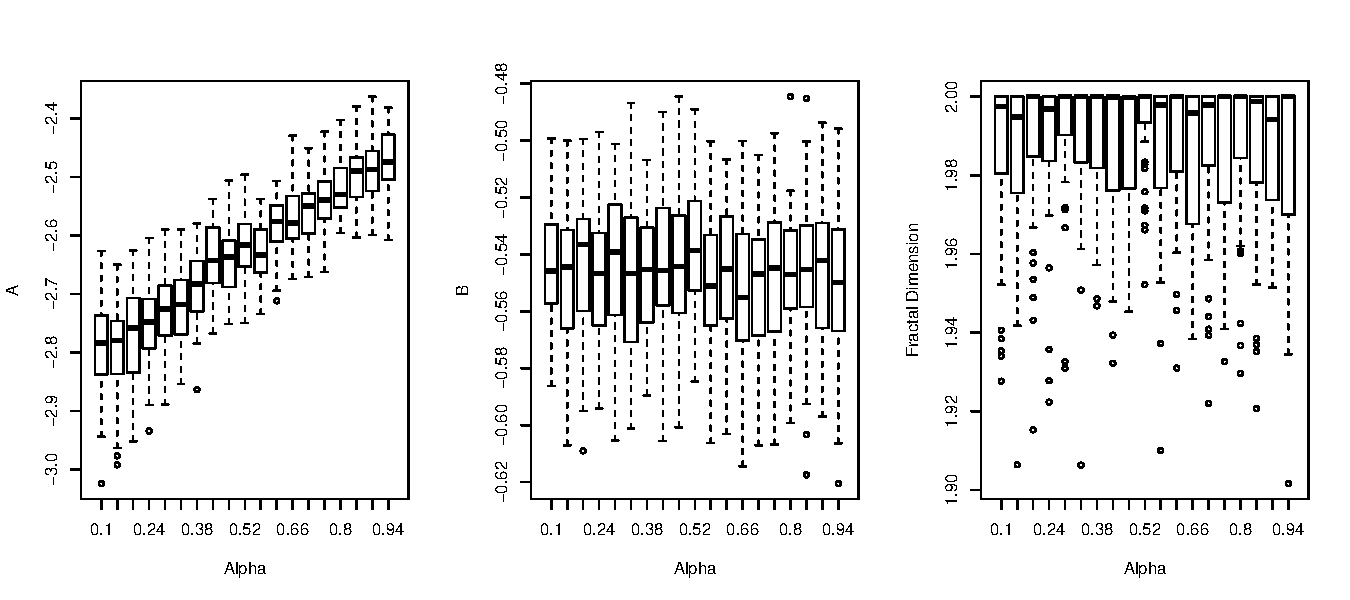
\includegraphics[height = 3in, width =6in, keepaspectratio]{./figs/holder_coeffs-boxplots.pdf}
   
  \caption{Complexity coefficients and fractal dimension 
  plotted against the $\alpha$ parameters of the 
  random-phase Weierstrass function.  }
  % \end{picture}
    \label{fig:rp-weierstrass-boxplot}
  \end{center}
\end{figure}

Examples of the FBM and Cauchy process time series used in our simulation are shown in figure \ref{fig:cauchyplot}. 
The results are similar to those of the deterministic 
Weierstrass function and both the complexity coefficient 
$B$ and $\hat D$ change linearly with the H\"older class
parameter. Also similar to the results for the Weierstrass 
function, the coefficient $A$ has a non-linear relation to $\alpha$.  
\begin{figure}[!htbp]
  \begin{subfigure}[b]{0.49\textwidth}
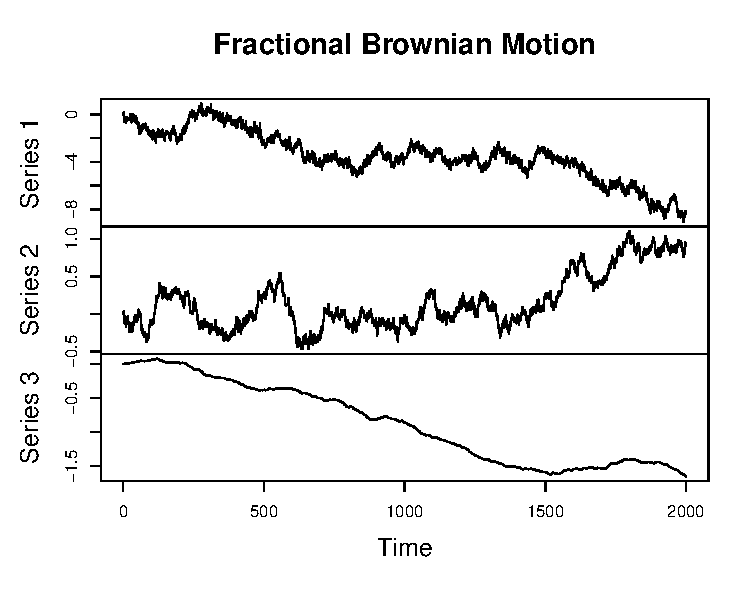
\includegraphics[width = 0.9\linewidth, height = 3in]{./figs/fBm-coeffs-plot.pdf}
    % \caption{Functions without added noise.}
    % \label{fig:fBmplot}
  \end{subfigure}
  \hfill
  \begin{subfigure}[b]{0.49\textwidth}
  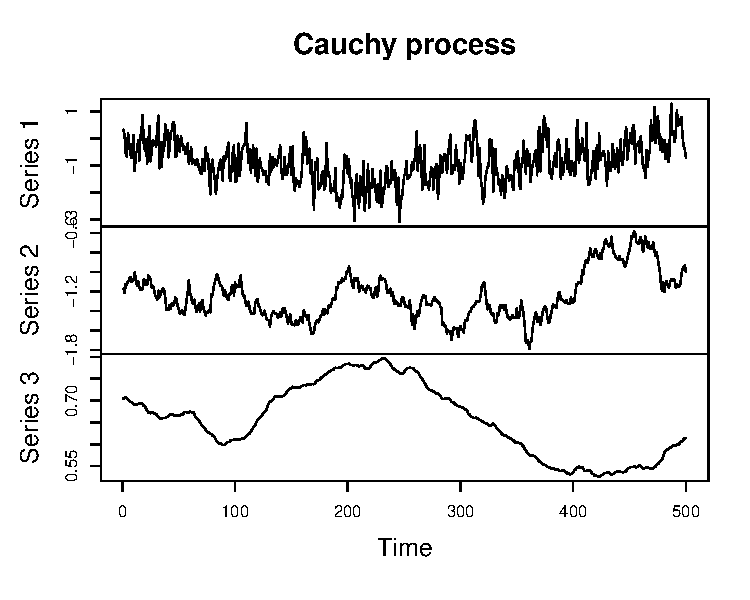
\includegraphics[width = 0.9\linewidth, height = 3in]{./figs/cauchy-plot.pdf}
    % \caption{Functions without added noise.}
    
  \end{subfigure}
  
  \caption{Fractional Brownian motion and the Cauchy process with $\alpha = \{ 0.20, 0.42, 0.80 \}$. The Cauchcy $\beta$ parameter was 
  held constant.}
  \label{fig:cauchyplot}
\end{figure}

\begin{figure}[!htbp]
  \begin{center}
  % \begin{picture}(60,60)
  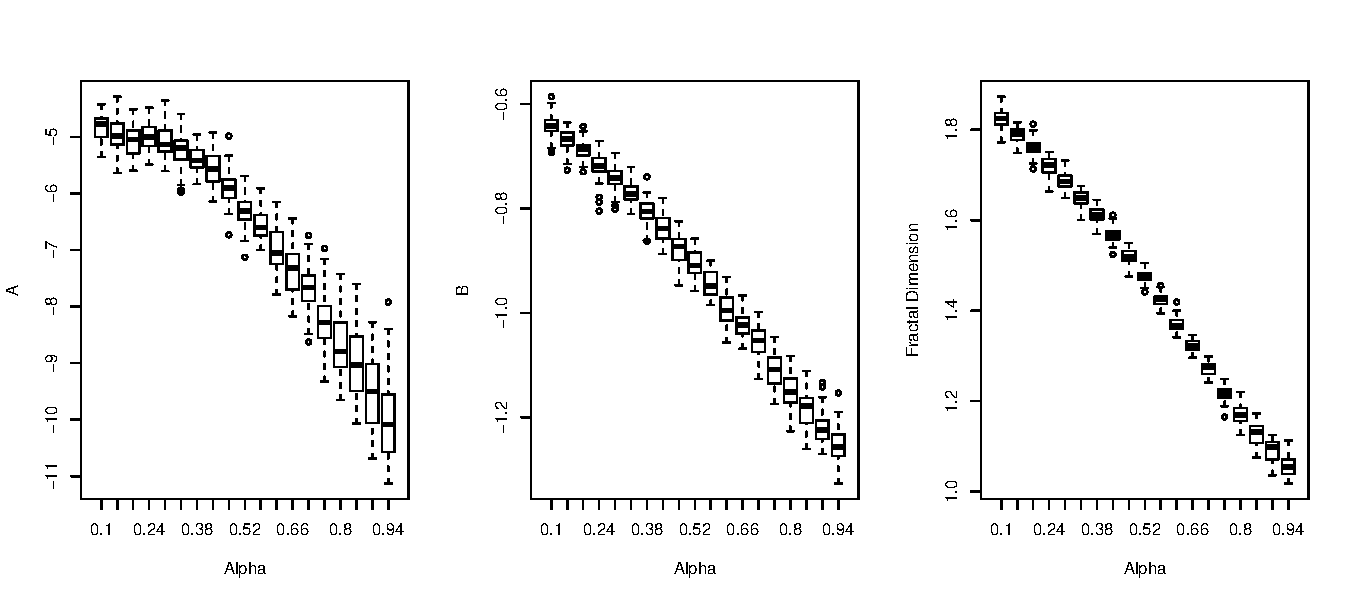
\includegraphics[height = 3in, width =6in, keepaspectratio]{./figs/fBm-coeffs-boxplots.pdf}
  % \end{picture}
  \end{center}
   \label{fig:fbm-boxplots}
  \caption{Complexity coefficients and fractal dimension plotted against the $\alpha$ coefficients of fractional Brownian motion.} 
\end{figure}

\begin{figure}[!htbp]
  \begin{center}
  % \begin{picture}(60,60)
  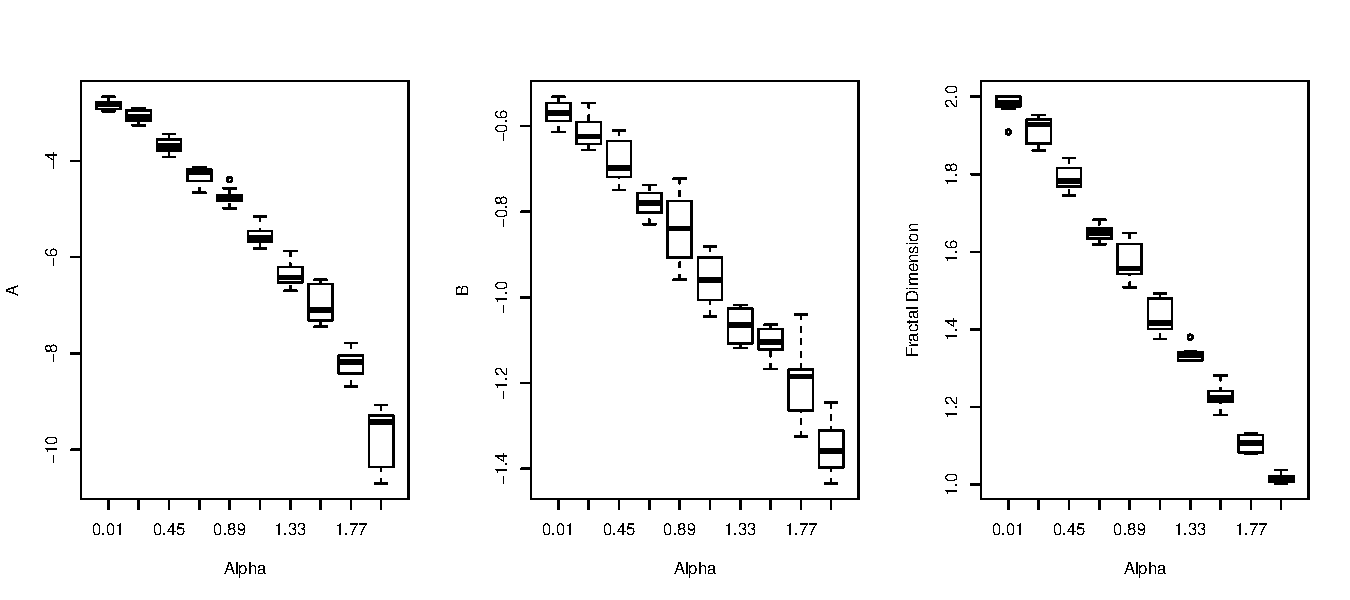
\includegraphics[height = 3in, width =6in, keepaspectratio]{./figs/cauchy-boxplots.pdf}
  % \end{picture}
  \end{center}
  \caption{Complexity coefficients and fractal dimension plotted against the Cauchy process $\alpha$ coefficient.} 
     \label{fig:cauchy-boxplots}
\end{figure}

The Cauchy process has two parameters, $\alpha$ determines
fractal dimension and the parameter $\beta$ determines 
the Hurst coefficient, or the long range correlation of the 
process. 20 simulations of the Cauchy process were generated
on a $10 \times 10$ grid of parameters $\alpha, \beta$
for $0 < \alpha < 2$ and $0 < \beta < 1.5$. 
In figure \ref{fig:cauchy-alpha} plots the mean value of the complexity coefficients as the long-range parameter 
$\alpha$ changes. Differences in the $\beta$ parameter show no effect the estimate of the complexity coefficients or the fractal estimator. 

\begin{figure}[!htbp]
  \begin{center}
  % \begin{picture}(60,60)
  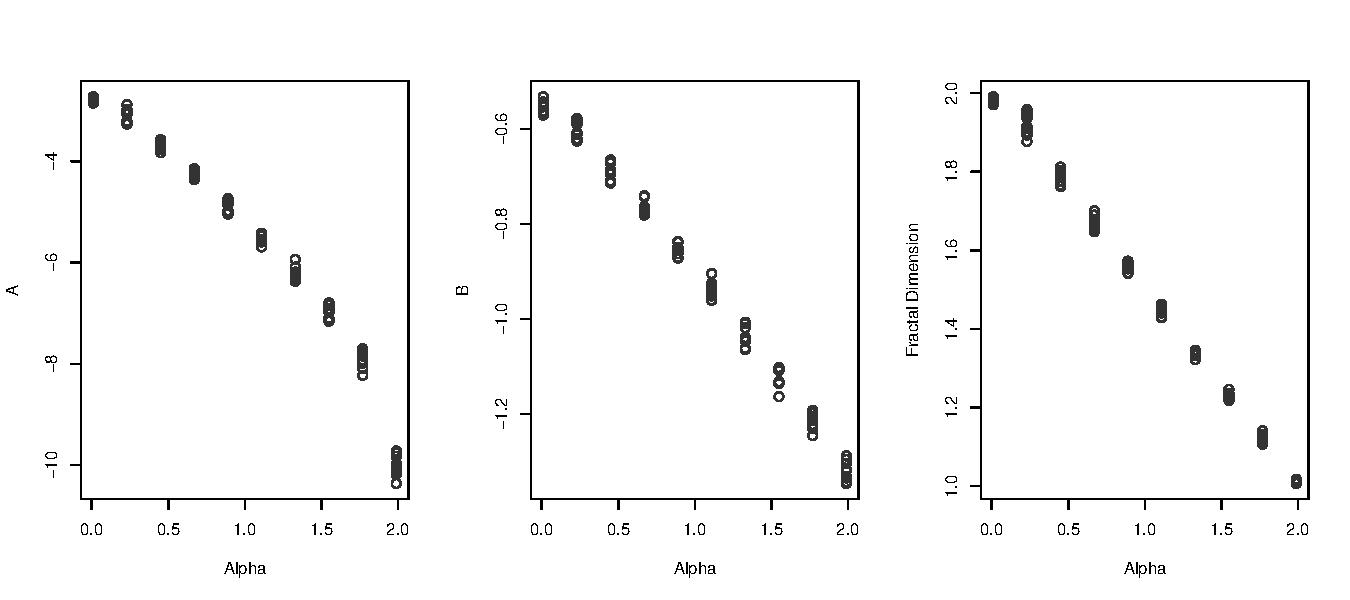
\includegraphics[height = 3in, width =6in, keepaspectratio]{./figs/cauchyalpha-scatterplots.pdf}
  % \end{picture}
  \end{center}
  \caption{The mean value of the complexity coefficients and fractal dimension plotted against the Cauchy process $\alpha$ coefficient.}
   \label{fig:cauchy-alpha}
\end{figure}

\begin{figure}[h]
  \begin{center}
  % \begin{picture}(60,60)
  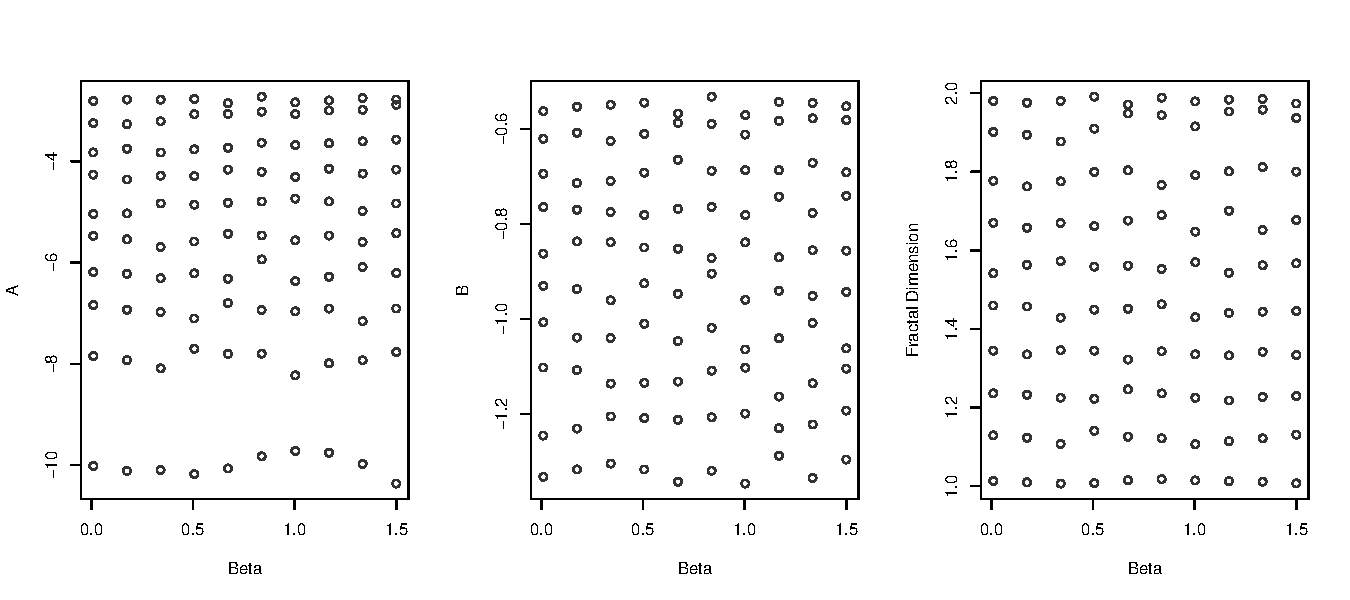
\includegraphics[height = 3in, width =6in, keepaspectratio]{./figs/cauchybeta-scatterplots.pdf}
  % \end{picture}
  \end{center}
  \caption{The mean value of the omplexity coefficients and fractal dimension plotted against the Cauchy process $\beta$ coefficient.}
 \label{fig:cauchy-beta}
\end{figure}

Figure \ref{fig:cauchy-beta} shows another view of 
the complexity coefficients plotted against 
changes the Cauchy process parameter $beta$. The complexity 
coefficient $B$ and fractal dimension clearly preserve 
the grid from the parameter space -- for a fixed 
$\beta$, the parameter varies linearly with $\alpha$. The 
$\beta$ parameter controls the long-range dependence of 
the Cauchy process and the plots indicate that 
the complexity coefficients, like fractal dimension,
measure a local, not global, property of a function.


Although these results are intended to be exploratory, for 
three of the four functions there is strong evidence that
the complexity coefficient $B$ behaves similarly to the 
variogram estimator of fractal dimension. The complexity 
coefficient $A$ does not seem to add much information 
for the three cases in which there was a linear relation between 
 $B$, $\hat D$, and the parameter determining the 
 H\"older exponent of the function, $\alpha$. 
 On the other hand, our initial example of simple functions and the random-phase Weierstrass functions appears shows a relationship between the intercept 
coefficient $A$ and fine-scale noise. These results are for a small set of processes with well-known behavior. A comparison of the complexity coefficient $B$ and fractal estimators on a wider variety of time series might show whether this relation holds under a wider range of conditions.






















\chapter{Seizure Prediction}

Electroencephalograms(EEG) capture the electromagnetic 
potential of similarly aligned neurons firing in unison. Although a number of correlations between 
EEG and physiological phenomena have been found the relation between EEG and neural circuitry dynamics are still not well-understood \cite{eeg}. 
one difficulty is relating in vitro behavior of individual neural cells with in vivo behavior of both local and global neural dynamics.  
For a neuropathological condition like epilepsy, 
the challenge is to relate global spread of 
synchronized firing to local cellular mechanisms.

In this chapter, we analyze EEG data gathered 
from a group of mice afflicted with a genetic 
mutation that causes early onset epilepsy similar to 
Dravet syndrome. This was an exploratory study to assess how well stimulus-induced seizures could be predicted and to find those features correlated with the likelihood of a seizure. 

The study of complex biological signals like EEG 
was one of the motivations for developing the 
$\varepsilon-$complexity feature. EEG are non-stationary
signals that exhibit transient waveforms and apparent regime changes over relatively short periods of times. In the context of dynamical systems, a regime change describes an alternation between semi-stable states 
\cite{lorenz2006}. While we do not assume the brain dynamics can be described as a non-linear dynamical system, the term is useful for characterizing the
observed behavior of EEG signals. 

A common method of analyzing EEG is to compute some set of features on the raw signal and use averages of the features over fixed windows. The procedure 
serves as a way of reducing the high-dimensional 
EEG signal and extracting a more interpretable
feature set. One drawback of this method is that the process of averaging over arbitrary windows may obscure important features associated with the varying dynamics of the brain. 

Previous studies have used a change-point detection algorithm applied to the raw EEG signal 
to segment and cluster these varying brain states, 
for example, the sleep states of neo-nates\cite{pirya2009}.
The $\varepsilon-$complexity feature is meant to capture an intrinsic feature of the signal. As shown in 
Chapter 4, the feature may also be related to the 
fractal dimension of a signal which Gneiting describes
as a second order statistical property of 
a signal through its relation to the variogram or 
correlation function\cite{gneiting2012}. 

In this chapter, we design a classifier that modifies
the typical feature extraction method segmenting the signal based on the $\varepsilon-$complexity coefficients. 
We compare classification accuracy on a dynamically segmented
set of features to several models that uniformly segment the feature set. For each of these models, we 
attempt to predict seizures based on features 
extracted from individual EEG channels rather than from the full set of six. The set of EEG channels correspond to specific functional regions of the brain.  
Feature extraction and classification based on individual channels allows us to make more fine-grained inferences about the combination of feature and region that are associated with a seizure response.


% The $\varepsilon-$complexity feature was develope with 

% The ECoG -- which I will refer to simply as EEG --
% signal captures changes in field potential caused by large 
% groups of aligned neurons firing synchronously. The LFP sensors
% capture a signal from a smaller cluster of neurons.

% a way to detect changes in the underlying dynamics that generate some signal. Specifically, the analysis of EEG was a motivating test case. EEG signals measure changes in 
% electrical potential generally at the outer layer or cortex of the brain. 

% \section{Seizure Prediction}


\section{EEG Data}

The EEG data gathered from 4 mice with a genetic 
mutation in the voltage-gated sodium channel gene Scn1a 
a similar mutation to that causing Dravet syndrome 
The mutation results in early onset epileptic seizures \cite{ito2013}.
The mice were equipped with 4 electrocortical(ECoG) sensors --intracranial sensors placed directly on the brain cortex --  
along with 2 local field potential (LFP) sensors located 
 in the thalamus.  
The mice were genetically modified to produce a light sensitive protein, an opsin, allowing for direct stimulation of neurons with a laser pulse train. 

% \begin{figure}[!htbp]
%   \begin{center}
%   % \begin{picture}(60,60)
%   % ./figs/coeff-interp-simple-functions1.pdf
%   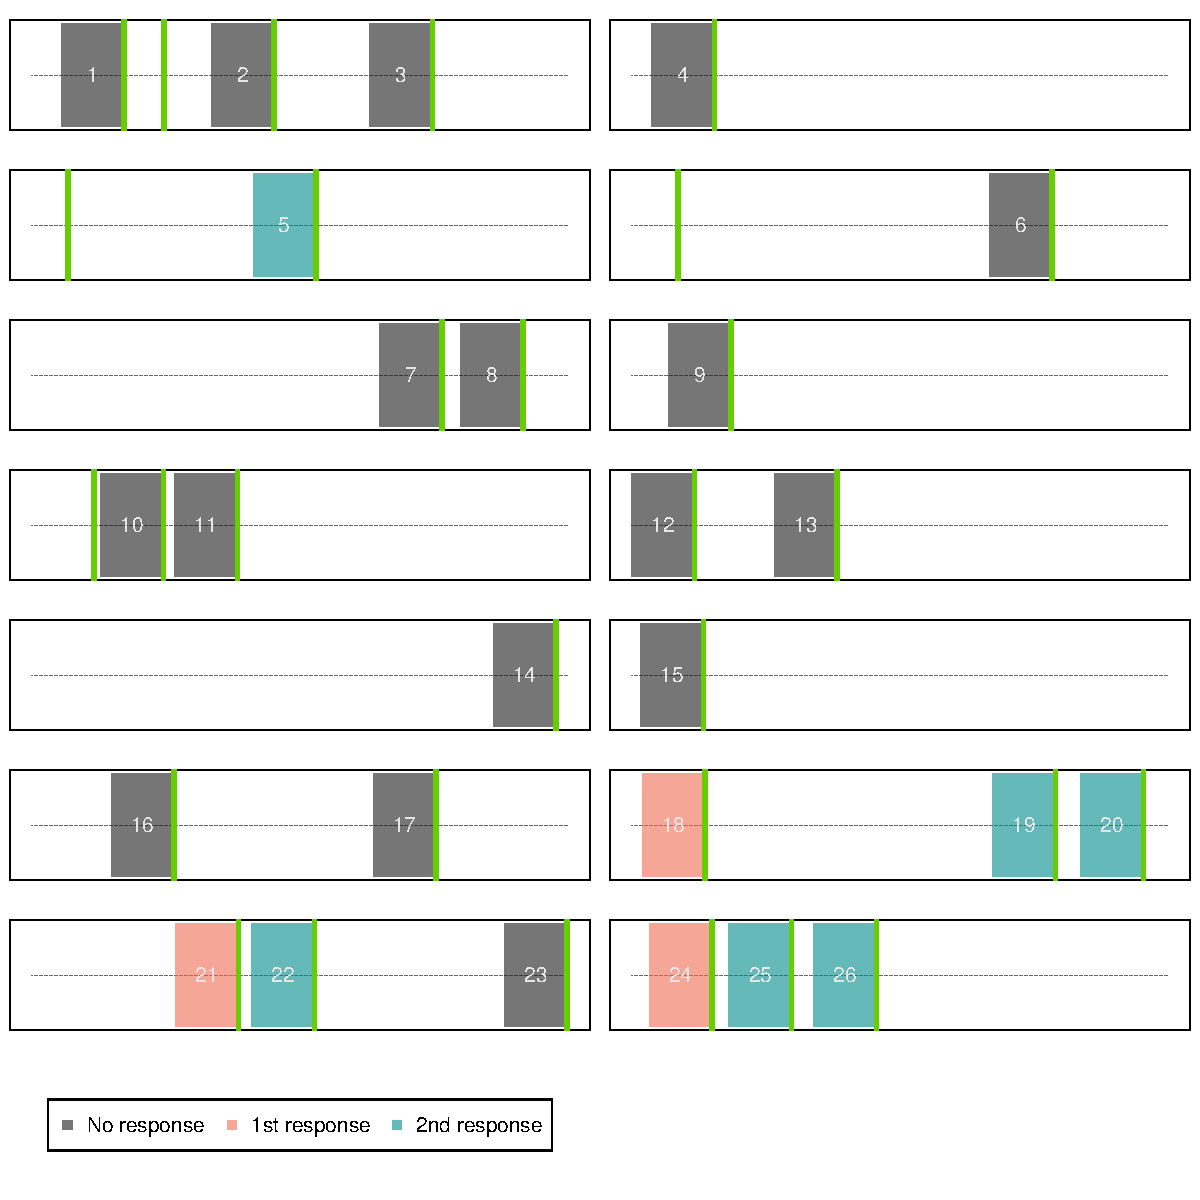
\includegraphics[width = \textwidth, keepaspectratio]{./figs/trialplot.pdf}
%   % \end{picture}
%   \end{center}
%   \label{fig:trialplot} 
%   \caption{Schematic plot of trial data. Each rectangle 
%            represents a single time period. The green 
%            vertical bars indicate applications of the stimulus.}
% \end{figure}

Data was gathered from 13 distinct time periods during which the was applied one to four times. 
4-minute segments preceding the stimulus were used as the final set of 26 trials. The results of each 
trial was were coded as either a seizure, which 
we refer to as a positive response, or no seizure. 
Coding was based on the visible response of the 
mouse. The EEG signals around the stimulus period were also visually examined to check the accuracy of the coding.

The EEG was sampled at 1220.7 Hz and
a bandpass filter removed frequencies below 0.5 Hz and greater
than 300 Hz. A notch filter was applied at 60 Hz and its harmonic frequencies. 


\section{EEG Features}
We selected a feature set consisting of standard 
spectral characteristics along with a few additional 
features. The power in frequency bands 
delta, theta, alpha, beta, and gamma was calculated 
as the integral of the spectral density $f(\lambda)$ 
computed as a smoothed periodogram. For example, 
delta band power, $\delta B$, corresponds to 
the frequency band $0.5-4Hz$ and integrates  
$f(\lambda)$ over over this interval
\[
  \B = \int_{0.5}^{4} f(\lambda) d\lambda. 
\]
The frequency bins corresponding to the remaining bands are, 
in order,$ 4-8Hz, 8-12Hz, 12-30Hz, 30-100Hz$. 

Additional features were selected based on two tests.
A set of non-linear features including sample entropy,
and permutation entropy, spectral entropy, a Hurst 
parameter estimator and fractal dimension along with wavelet coefficients  and variance were tested for their ability to discriminate between the same two groups of simulations used in Chapter 3 to test the approximation methods used in estimating complexity coefficients. Based on these results, spectral entropy, fractal dimension, the Hurst parameter and the wavelet coefficients, along with the spectral band power features and the complexity coefficients were computed on the EEG. In informal testing
with a baseline classification model, the wavelet coefficients did not improve classification results and were removed from the final feature set. Given more data, feature selection might have been better performed through cross-validation on a training set. On the other hand, one of our goals was to work with a reduced feature set that was more readily interpretable. 

We have defined most of the features used in classification in Chapter 2. Spectral Entropy is a measure of the distribution in the spectrum of a signal. 
\[  
  SE = - \int_{-\pi}^{\pi} f_x(\lambda) \log f(\lambda) d \lambda.
\]
The Hurst parameter was estimated using the corrected empirical Hurst exponent\cite{weron2002}.  
 
All features were calculated on non-overlapping 2-second intervals. The final list of feature used in classification was 
\begin{enumerate}
\item Delta, theta, alpha, beta, gamma 
\item Spectral entropy 
\item Hurst parameter
\item Variance
\end{enumerate}

The complexity coefficients were used in our segmentation 
classifier but not as a feature. The variogram estimator of fractal dimension, $\hat D$ was also computed but was omitted from the final models as the feature appeared closely correlated with the complexity coefficient $B$. 

% Figure \ref{fig:trialplot}
% is a schematic picture of the trial periods. 
% There are several trials that did not follow a previous 
% seizure, and below we compare whether the features
% for these trials appear to come from a distribution 
% similar to the seizure response trials that followed 
% a previous seizure.

% Segmentation on the complexity coefficients is a 
% depends on the 
% Initially, the features were computed on 4 second intervals but at this resolution no change points were detec

\section{Segment Classifier}

% Although raw EEG time series values are used in some classification approaches, when using neural-network based classifiers for example,
%  a common approach is to compute a set of features on the time series and use 
% these features as predictors. Using features rather than raw time series 
% serves to reduce the dimensionality of the data. 
Whether it is spectral features or $\varepsilon-$complexity 
features, the mapping of the raw data to the 
features results both in a dimensionality 
reduction and an averaging over some variation and structure 
in the data. That is, there is a trade-off between losing 
important variation in the data and reducing the dimension
of the raw input. In our approach, we compute features 
in three basic steps. Features are computed at a relatively 
fine resolution for each EEG channel. Given an 
individual channel, the time series formed by the features
is segmented based on changes in the complexity coefficients. 
The weighted averages of the features set on these segments is
used as a training set for the classifier. 


% We selected a small set of features for our classifier. 
% These included the band power of the  
% frequency bands delta, theta, alpha, beta and. 
% Spectral features need 
% to be computed over a windowed section of the time series 
% that is some multiple of the lowest frequency being computed 
% in order for the power estimates to have some statistical 
% validity. So using spectral features inherently reduces 
% the dimensionality of the data, for example, from several 
% thousand points a set of six values representing the 
% band power of some window of frequencies will be computed. 
%  Features including the 
% complexity coefficients are computed on 2 second intervals. 
% Change-points in the complexity coefficients are then 
% used to segment the features. The final predictor 
% is the mean of the features computed on each segment.
% The basic steps used are outlined below.

 %   \begin{algorithm}[!htbp]
 %    \label{alg:segmenet}
 %  \caption{Single channel segment classifier \label{alg:ecomplex}}
 %  \DontPrintSemicolon
 %  \SetAlgoLined
 %  \SetKwInOut{Input}{Input}\SetKwInOut{Output}{Output}
 %  \Input{$ \mathcal{F} $ a set of multivariate time series
 %      $\textbf{f} $ corresponding of length $N$.}
 %  \Input{$\mathcal{L}_f$ a set of labels $l_f$ for each time series 
 %  $ \textbf{f} $ }
 %  \Input{$\mathcal{X}$ a set of time series $x_f$ of length $N$ 
 %  used to partition each $\textbf{f}$.} 
 %  \Output{$\mathcal{M}$ a trained classification model.}
 %  % \tcp{initialize array}
 %   % Initialize the array epsilons $\leftarrow [0]$   \;
 %  \BlankLine 
 % \ForEach{$f$ in $\mathcal {F}$} {    
 %    % \tcp{initialize array}    
 %   Compute the change points for $\mathcal{x}_f$
 %      $p_f \leftarrow$  change_pts($\mathcal{X}_f$)
 %   Segment $f$ on change points $x_f$
 %     $\{ f \} \leftarrow f$
 %    \ForEach{$f$ in $\mathcal{F}$} {
 %      % \tcp{Compute the approximation error}
 %        Compute the approximation error \\ 
 %        $\varepsilon_{h,f} \leftarrow 
 %       \frac{1}{N}\norm{f_h - X_{h} }^2$.  \;
 %      % mse\leftarrow \varepsilon_{h,f}$
 %    } 
 %     Find minimium error over all $f$  \\
 %     epsilons$_h$ $\leftarrow \min \varepsilon_{h,f}$. \;
 %  }
 %  Fit a least squares linear model \\
 %   $A,B$ $\leftarrow$ lm(epsilons$_h$ $ \sim \{ \mathbb{S}_h \} $.) \;
 %  \end{algorithm}

\begin{enumerate}
  \item For each channel compute set of features
        on regular intervals including 
        $\varepsilon-$complexity.
  \item For each channel, compute the change points 
        in $\varepsilon-$complexity. 
  \item For each trial, segment all features using the change point 
        set computed in the previous step. 
  \item Compute the mean of each feature on the 
        segments. 
   \item Label the means of the segments 
         in a training 
         set with the label of the full time 
         series and use this set to train 
         a classifier.
   \item Train a classifier on the means of the 
         segments. 
  \item  For the means of the segmented test set,
         compute the class probability of each 
       segment using the trained 
         classifier. 
  \item  For each trial use the prediction probabilities of each segment weighted by segment length to compute the final class probability.
\end{enumerate} \label{alg:segment-alg}

In the case of a uniform partition of the features, this
the method is equivalent to simply using the average class probability for each segment to classify the trial.

In theory, any classifier, or several classifiers could be used in steps 5 and 6. We used a random forest classifier. The random forest is constructed from a large number of individual decision trees. For numeric data, the decision trees partition the feature space into $d-$dimensional rectangles each labeled with a class. The decision trees branches correspond to partitions of the feature space. For each branch, a subset of the features are chosen and the split is made in order to increase the class purity of each partition. The final prediction is based on the combined vote of the individual trees.  In addition to random selection of features, a random subset of observations are used to build each tree. This allows for an out-of-bag(OOB) estimate of the classifier 
accuracy which is calculated by classifying each observations using the set of trees which were built without seeing that observation \cite{breiman2001}.

\begin{figure}[!htbp]
  \begin{center}
  % \begin{picture}(60,60)
  % ./figs/coeff-interp-simple-functions1.pdf
  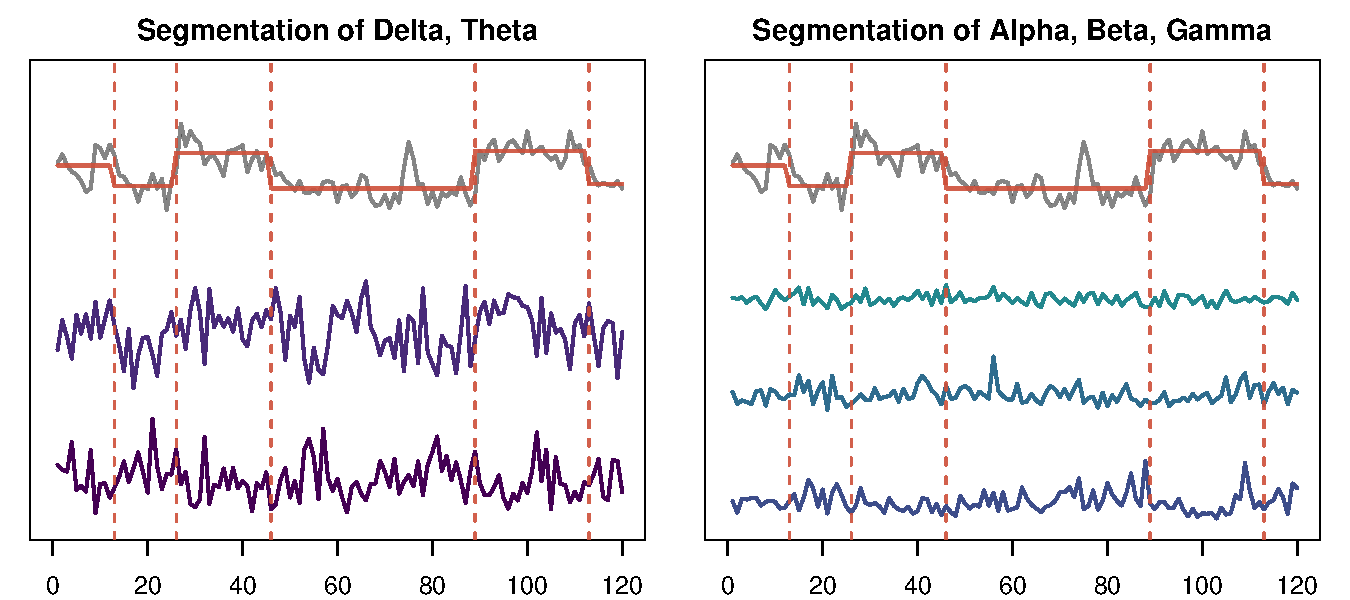
\includegraphics[width = \textwidth, keepaspectratio]{./figs/eeg-segment-plot.pdf}
  % \end{picture}
  \end{center}
  \label{fig:segplot} 
  \caption{Spectral features segmented on changes in the B complexity coefficient.}
\end{figure}

\section{Model Performance}

We begin by defining several terms we will be using to describe classifier performance. We term a seizure a 
positive response or simply a response. A  
\textit{true positive}  
is an accurate prediction of a seizure while a 
 \textit{true negative} is an accurate prediction of a non-response. 
The  \textit{sensitivity} of the classifier is then 
defined as the proportion of true positives to total 
positive and  \textit{specificity} is the total of true 
negatives to total negatives. We use the term accuracy to refer to balanced accuracy
\[
  \text{Balanced Accuracy} = \frac{\text{Sensitivity + Specificity}}{2}.
\] 
We also report AUC, or area under the ROC curve, see 
Figure \ref{fig:eegroc} for an example from two 
of the classifiers tested. The 'curve' is the plot 
of the sensitivty against the false positive rate or 
$1 - $specificity and a higher AUC indicates a better performing classifier.

We created a simple baseline classification model to compare to the segmented classifiers. The feature set for this model was the mean of each of the 8 features on the six channel resulting in 48 features. A random forest classifier was trained on these features and the out-of-bag classification results are reported in table \ref{tab:baseline}.

% Asymptotically this is an unbiased estimate the error on a

 \begin{table}[!htbp] \centering 
 
\begin{tabular}{@{\extracolsep{5pt}} cccc} 
\\[-1.8ex]\hline 
\hline \\[-1.8ex] 
 & Sensitivity & Specificity & Accuracy \\ 
\hline \\[-1.8ex] 
1 & $0.544$ & $0.935$ & $0.740$ \\ 
\hline \\[-1.8ex] 
\end{tabular} 
 \caption{Classification performance of baseline classifier.} 
  \label{tab:baseline} 
\end{table} 


% \begin{table}[!htbp]
% \begin{center}
%   \begin{tabular}{ | c | c |  c|} 
%   \hline 
%  Sensitivity & Specificity  &  Accuracy  \\ \hhline{|=|=|=|}
%   0.54  &  0.94     &    0.74  \\ \hline
% \end{tabular}  
% \caption{Prediction performance for baseline classifier.}
% \label{tab:baseline}
% \end{center}
% \end{table}

We compared six models to this baseline model. For each 
model a different partition scheme was used. For the models
using complexity coefficients we denote $A, B, A+B$ where 
each trial was partitioned based 
on change points detected in the corresponding complexity 
coefficients and the $A + B$ model is simply the union 
of the change points of both complexity coefficients. 
Three other models used regular partitions.   
Each trial was uniformly segmented into $8, 15$ or $30$ segments and we refer
to these models by the partition number. 

The performance of these models was assessed using 
5-fold cross-validation where balanced sets were used for the hold-out set for each fold. The reported results are based on 10 repetitions or bootstrap samples. Results for a larger number of repetitions, 50, were similar. We report to smaller sample to emphasize the relative sizes of the confidence intervals of the reported performance measures. In general, all models performed best on the LFP channels, 
here labeled channel 1 and 2. These sensors are located in the thalamus and measure the electrical potential of a small set of neurons. The best performing model was the regularly partitioned model with 8 segments followed by the model $A+B$.

\begin{figure}[!htbp]
  \begin{center}
  % \begin{picture}(60,60)
  % ./figs/coeff-interp-simple-functions1.pdf
  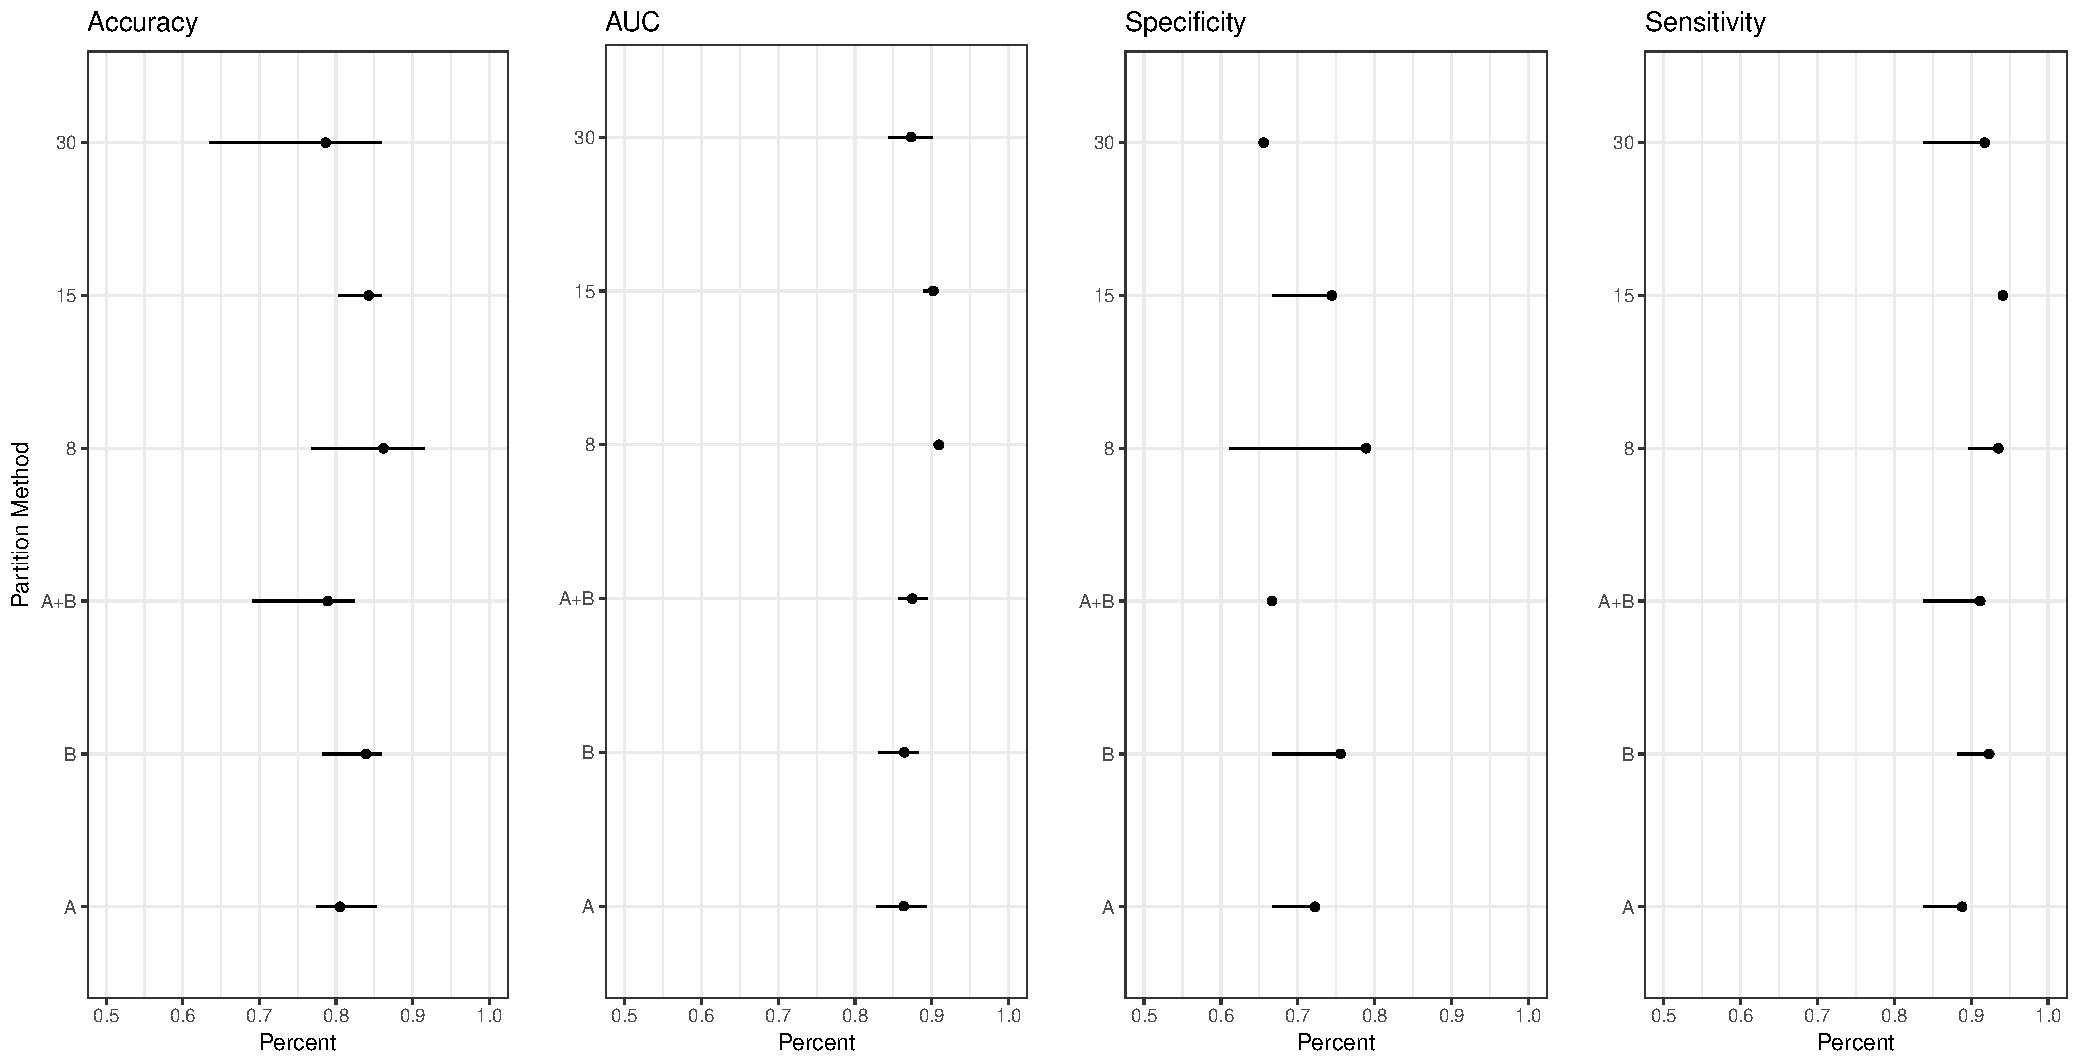
\includegraphics[width = \textwidth, keepaspectratio]{./figs/eeg-partition-diagnostic.pdf}
  % \end{picture}
  \end{center}
  \caption{Classification diagnostic values for each partition method for LFP channel 1.}
  \label{fig:eeg-diagnostic} 
\end{figure}

The performance measures for each classifier on channel 
1 are shown in figure \ref{fig:eeg-diagnostic}. The 
mean and 95\% confidence interval based on 10 
bootstrap classifications are reported.  All methods classified 
non-response trials well but the two better performing
 models -- model 8  and model $A+B$ -- 
had relatively high accuracy in classifying seizure responses: 76\% for model $A+B$ and 79\% for model 8. 

Classification is generally more difficult 
when classes are unbalanced, that is, when there are 
significantly fewer observations in the training 
set of one class compared to the other. Other 
than performing cross-validation on a balanced 
hold-out set, no other adjustments were made in 
the underlying random forest model or the 
threshold probability for selecting a class.  

% \begin{minipage}{0.45\textwidth}
\begin{table}[!htbp] \centering 
\begin{tabular}{@{\extracolsep{1pt}} ccccccc} 
\\[-1.8ex]\hline 
\hline \\[-1.8ex] 
 & Ch1 & Ch2 & Ch3 & Ch4 & Ch5 & Ch6 \\ 
\hline \\[-1.8ex] 
A & $0.76$ & $0.76$ & $0.70$ & $0.71$ & $0.57$ & $0.60$ \\ 
B & $0.78$ & $0.77$ & $0.70$ & $0.69$ & $0.60$ & $0.64$ \\ 
A+B & $0.84$ & $0.70$ & $0.69$ & $0.71$ & $0.59$ & $0.61$ \\ 
8 & $0.85$ & $0.81$ & $0.69$ & $0.71$ & $0.68$ & $0.82$ \\ 
15 & $0.79$ & $0.79$ & $0.73$ & $0.71$ & $0.73$ & $0.73$ \\ 
30 & $0.78$ & $0.80$ & $0.72$ & $0.71$ & $0.72$ & $0.84$ \\ 
\hline \\[-1.8ex] 
\end{tabular} 
  \caption{Balanced accuracy for each model and channel} 
  \label{tab:all-accuracy} 
\end{table} 
% \end{minipage}
% \hfill

% \begin{minipage}{0.45\textwidth}
\begin{table}[!htbp] \centering  
\begin{tabular}{@{\extracolsep{1pt}} ccccccc} 
\\[-1.8ex]\hline 
\hline \\[-1.8ex] 
 & Ch1 & Ch2 & Ch3 & Ch4 & Ch5 & Ch6 \\ 
\hline \\[-1.8ex] 
A & $0.64$ & $0.58$ & $0.46$ & $0.49$ & $0.23$ & $0.28$ \\ 
B & $0.66$ & $0.59$ & $0.48$ & $0.53$ & $0.36$ & $0.34$ \\ 
A+B & $0.76$ & $0.46$ & $0.46$ & $0.52$ & $0.28$ & $0.30$ \\ 
8 & $0.79$ & $0.68$ & $0.48$ & $0.51$ & $0.50$ & $0.69$ \\ 
15 & $0.69$ & $0.63$ & $0.52$ & $0.50$ & $0.62$ & $0.53$ \\ 
30 & $0.62$ & $0.67$ & $0.51$ & $0.49$ & $0.57$ & $0.76$ \\ 
\hline \\[-1.8ex] 
\end{tabular} 
  \caption{Specificity for all models and channels.} 
  \label{tab:specificity}
\end{table} 
% \end{minipage}

The balanced accuracy all models for each channel is shown in Table \ref{tab:all-accuracy}. All partition
schemes resulted in fairly high rates of accuracy for channels 1 and 2. The models with a higher number of 
partitions performed significantly better on the 
ECoG channels 3-6. On the other hand, accurate classification of seizures tailed off sharply for all ECoG channels as seen in Table \ref{tab:specificity}. 

\begin{figure}[!htbp]
  \begin{center}
  % \begin{picture}(60,60)
  % ./figs/coeff-interp-simple-functions1.pdf
  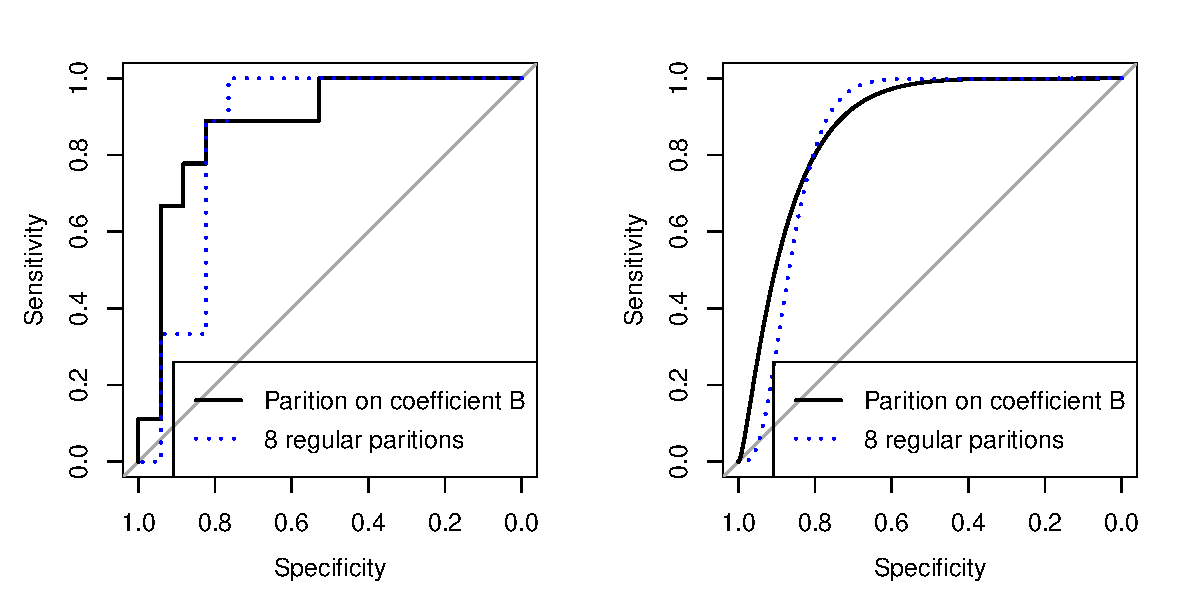
\includegraphics[width = \textwidth, keepaspectratio]{./figs/eegroc-comb.pdf}
  % \end{picture}
  \end{center}
  \caption{ROC curves and smoothed ROC curves
           for classification on channel 1 using 
           partitions on coefficient B and a regular partition into 
           8 segments.}
\end{figure}
\label{fig:eegroc} 
\section{Feature Importance}

As mentioned above, with only a small set of observations, 
improved classification on one or two instances
would affect the performance of the classifier.
Whether the model used here --
partitions based on complexity coefficients -- would be successful in other contexts remains to be seen. 
One of our assumptions was that arbitrary partitioning would average over changes variations in the features that corresponded to transient states. 
But whether the complexity coefficients capture significant
changes in the underlying dynamics that are useful for classfication might depend on both feature selection and the classification task. 

% \begin{table}[!htbp]
% \begin{center}
%   \begin{tabular}{ | c | c |  c| c | c | c |c| } 
%   \hline 
% Channel       &     1&    2 &    3 &     4 &     5 &    6  \\ \hline
% Partition Type    &       &      &     &     &  &  \\ \hhline{|=|=|=|=|=|=|=|}
% A    & 0.81 & 0.78 & 0.69 & 0.72  & 0.57  & 0.63  \\ \hline
% B    & 0.84 & 0.77 & 0.72 & 0.70  & 0.57  & 0.65  \\ \hline
% A+B  & 0.81 & 0.74 & 0.73 & 0.72  & 0.55  & 0.60  \\ \hline
% 8    & 0.86 & 0.84 & 0.73 & 0.72  & 0.74  & 0.75  \\ \hline
% 15   & 0.85 & 0.81 & 0.74 & 0.73  & 0.75  & 0.75  \\ \hline
% 30   & 0.79 & 0.75 & 0.76 & 0.77  & 0.72  & 0.77  \\ \hline
%       \end{tabular}  
% \caption{Balanced classification accuracy for each partition method 
%          and each channel.}
% \label{tab:error-allch}
% \end{center}
% \end{table}

% Table created by stargazer v.5.2 by Marek Hlavac, Harvard University. E-mail: hlavac at fas.harvard.edu
% Date and time: Sun, Jun 25, 2017 - 10:27:00 PM
 
A goal of our study was to determine features  
predictive of seizures. The selection of a reduced
the feature set and prediction on isolated channels
allow us to measure the feature importance for 
classification for each sensor location.
The distributions of features for response and non-response trials are looked
at below. Examining the one-dimensional distribution of the feature may not reveal interactions between the features in higher dimensions. 
On the other hand, decision trees divide up the feature space in complex ways and the final ensemble votes are what determines the classification outcome. 
In theory, those features found to be useful in classification will not necessarily be identifiable with basic summary statistics such as the mean, median or variance. However, for our data, the features used by the best predictors were associated with significant distributional differences across classes.
%  in particular 
% the features trained on predictors trained on the LFP channels 1 and 2. 

\begin{figure}[h]
  \begin{subfigure}[b]{0.45\textwidth}
      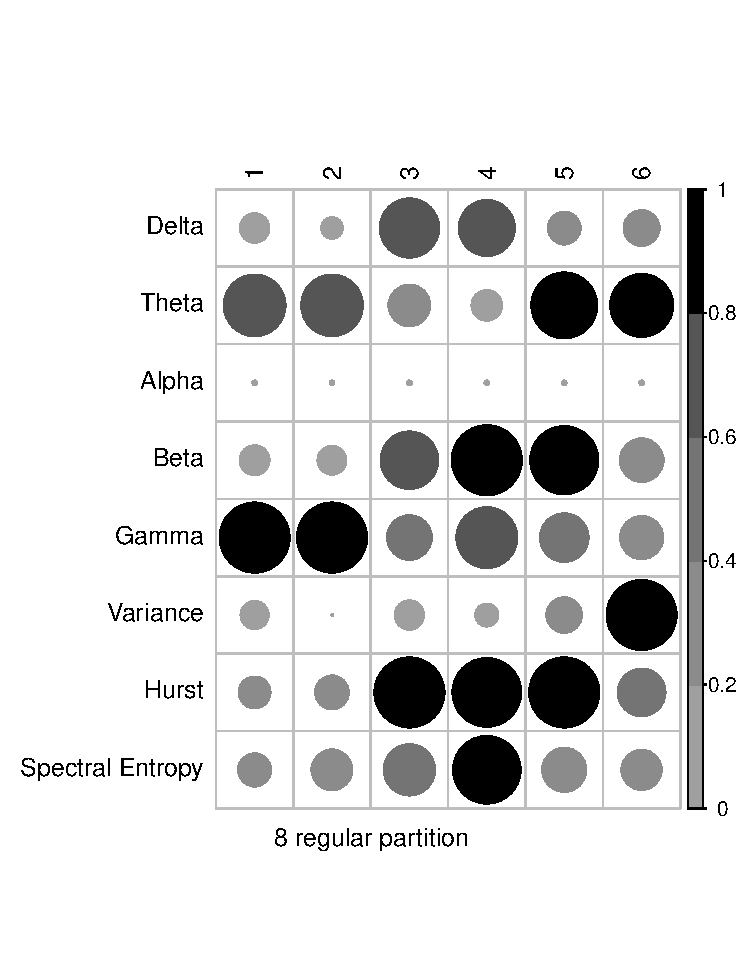
\includegraphics[width = \linewidth, keepaspectratio]{./figs/eeg-vec-corrplot.pdf}% \end{picture}
    % \caption{Functions without added noise.}
    % \label{fig:corrplot}
  \end{subfigure} 
  \hfill
  \begin{subfigure}[b]{0.45\textwidth}
    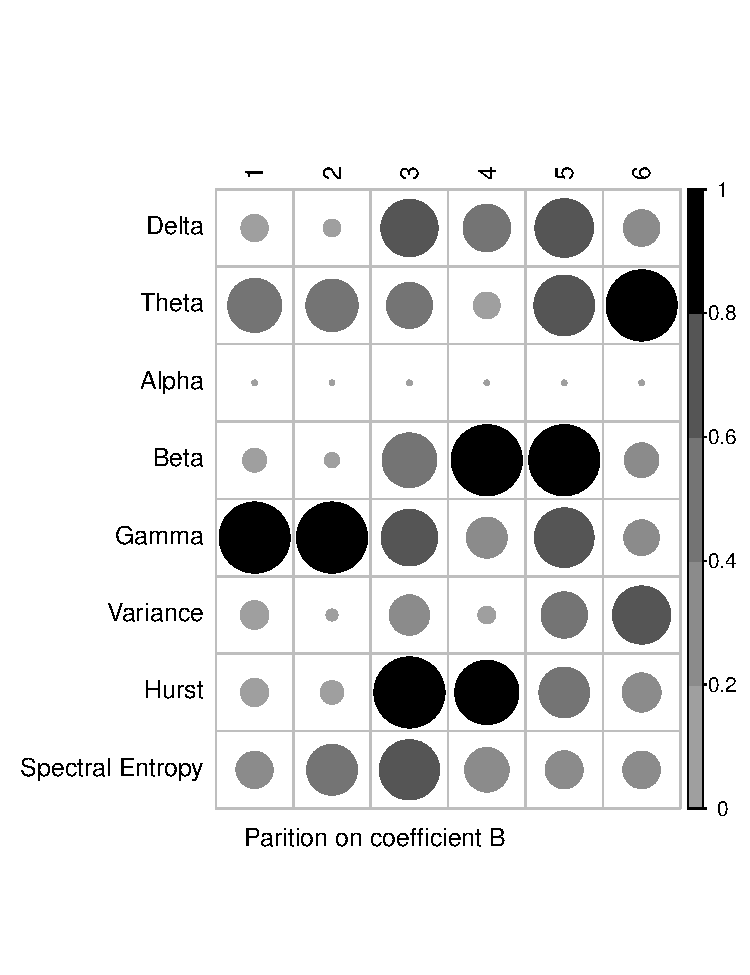
\includegraphics[width = \linewidth, keepaspectratio]{./figs/eeg-AB-corrplot.pdf}% \end{picture}
  % 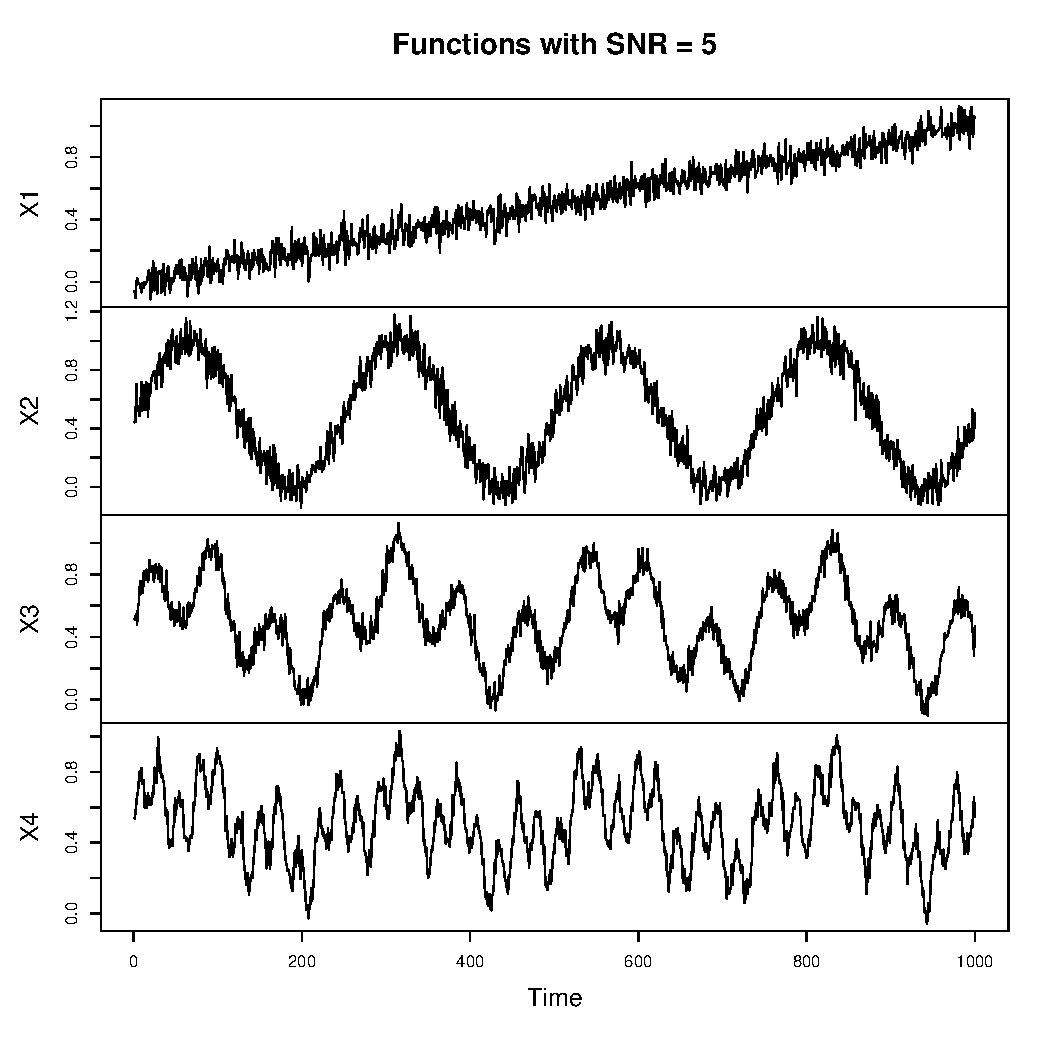
\includegraphics[width = 0.9\linewidth, height = 3in]{./figs/coeff-interp-simple-functions1.pdf}
    % \caption{Functions without added noise.}
      \end{subfigure}
  \caption{Variable importance for
   partition methods normalized to 
  a $[0,1]$ interval for each channel.}
    \label{fig:corrplot}
\end{figure}

We report the mean variable importance of the random forest classifiers trained during cross-validation. Variable importance is determined by the mean decrease in the
class Gini index when branches are made on a given feature
\cite{breiman2001}. Informally, variable importance
measures how well a feature divides response trials from non-response
trials. In Figure \ref{fig:corrplot} we show the variable 
importance for the two best performing models $A+B$ and the 
model $8$. We have normalized variable importance to a $[0,1]$ interval for each model and
channel so the figure shows the relative importance of the variable for each model. There is a common pattern in the variable importance across the two models. Gamma and theta bands have the highest importance for the best performing models, those trained on the LFP channels 1 and 2. 
Both partition methods also show increased importance for beta on channels 4 and 5 and increase the importance of the Hurst coefficient for channels 3 and 4. 

\begin{figure}[!htbp]
  \begin{subfigure}[b]{ \textwidth}
  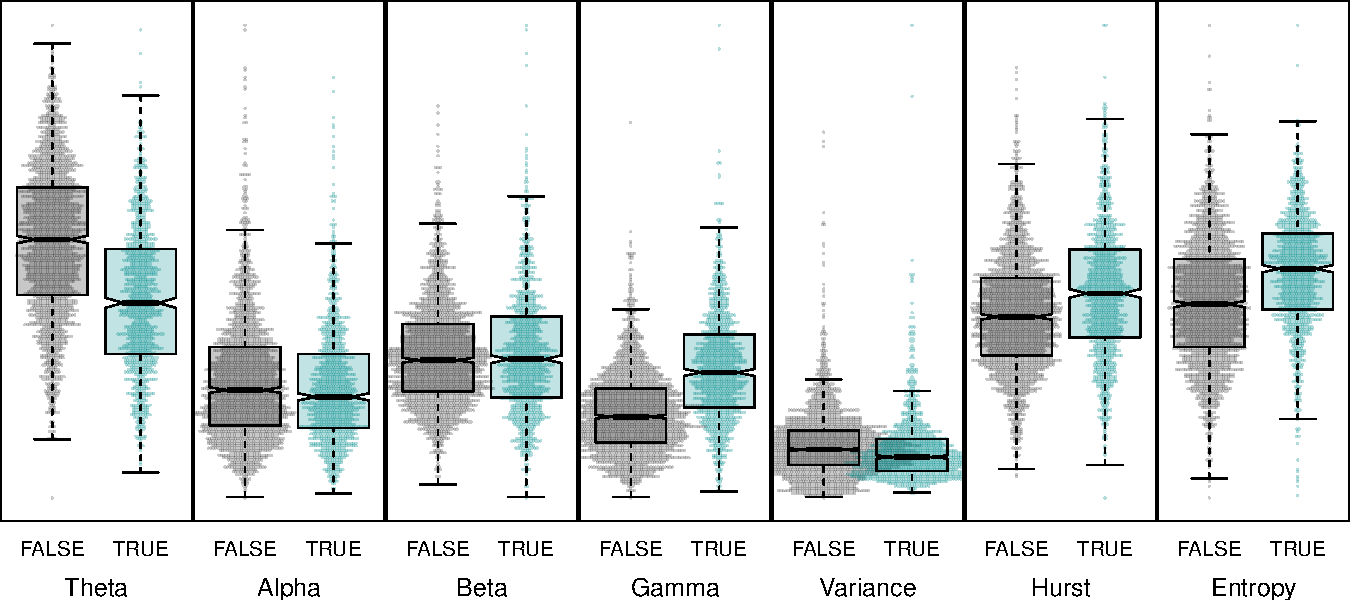
\includegraphics[width = \textwidth, keepaspectratio]{./figs/eeg-boxplot1.pdf}
    % \label{fig:corrplot}
  \end{subfigure} 
  \hfill
  \begin{subfigure}[b]{\textwidth}
  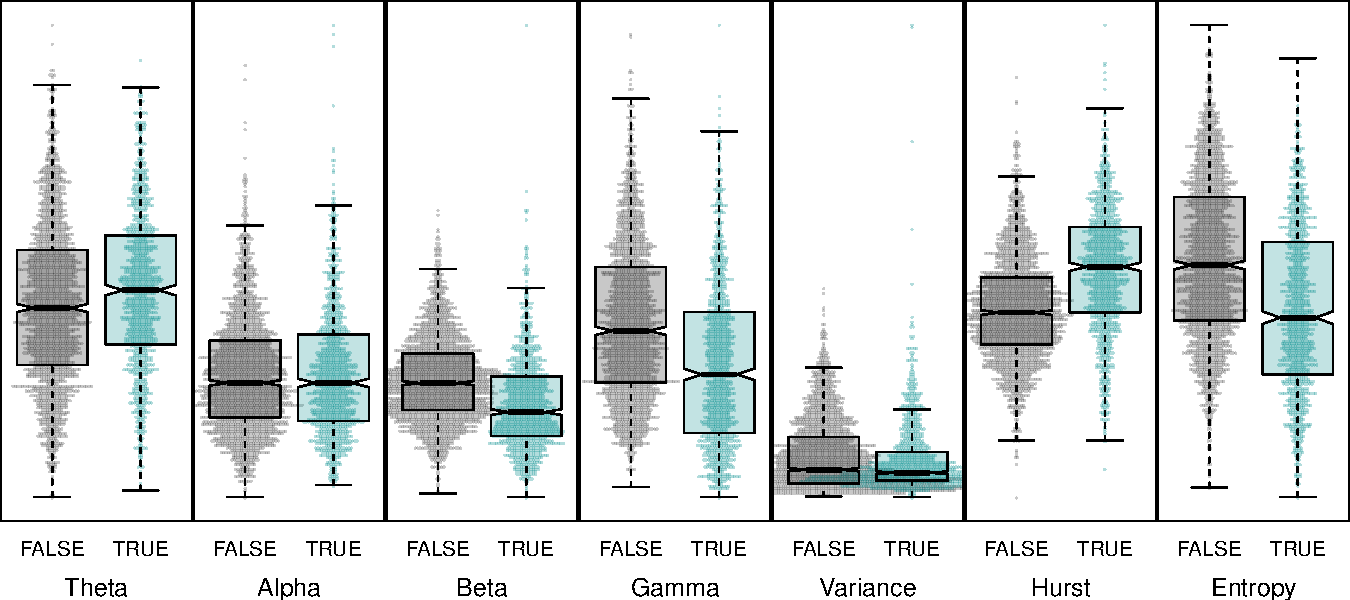
\includegraphics[width = \textwidth, keepaspectratio]{./figs/eeg-boxplotch3.pdf}
  % 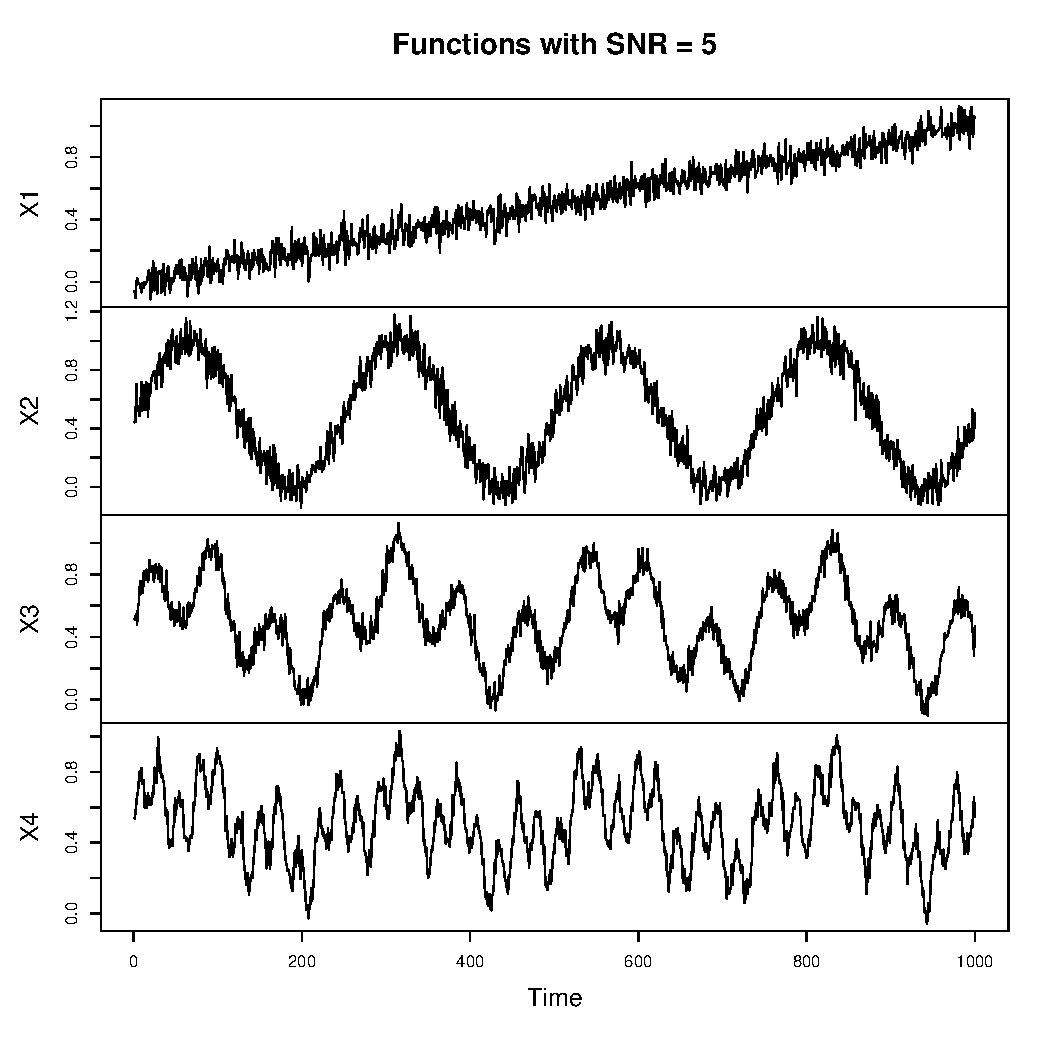
\includegraphics[width = 0.9\linewidth, height = 3in]{./figs/coeff-interp-simple-functions1.pdf}
    % \caption{Functions without added noise.}
      \end{subfigure}
  \caption{Feature distribution for channels 1 and 3.}
  \label{fig:boxplot}
\end{figure}

% \begin{figure}[!htbp]
%   \begin{center}
%   % \begin{picture}(60,60)
%   % ./figs/coeff-interp-simple-functions1.pdf
%   % \end{picture}
%   \end{center}
%   \label{fig:eegroc} 
%   \caption{Feature distribution for channel 1.}
% \end{figure}

% \begin{figure}[!htbp]
%   \begin{center}
%   % \begin{picture}(60,60)
%   % ./figs/coeff-interp-simple-functions1.pdf
%   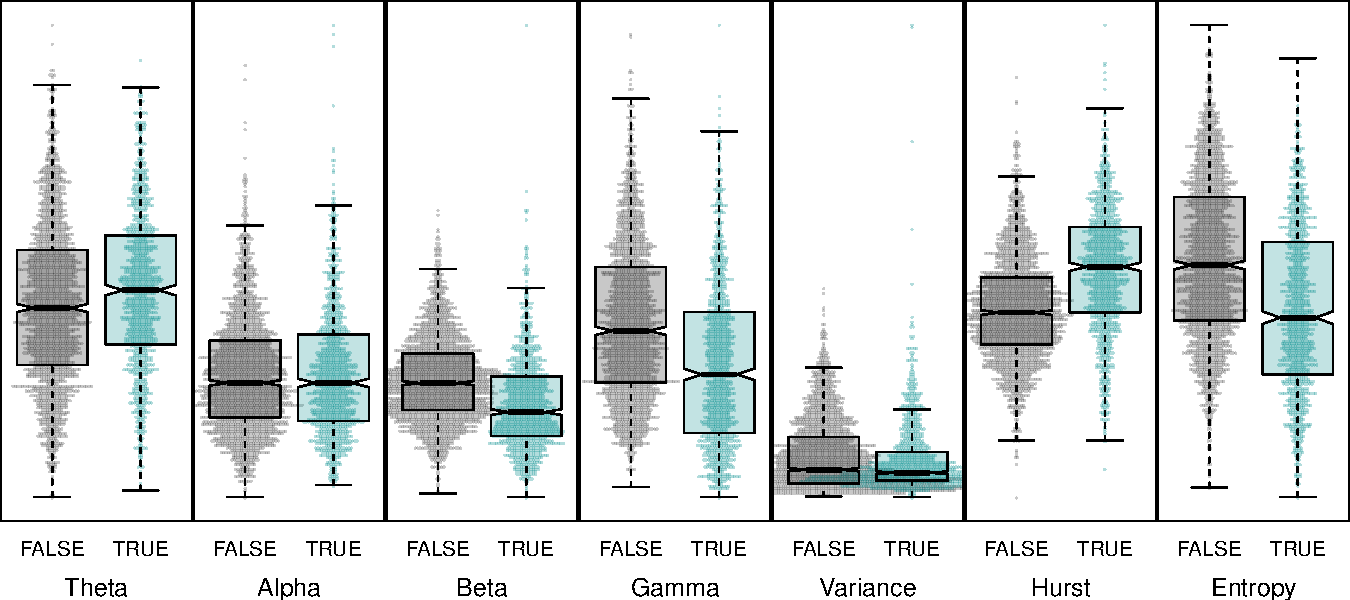
\includegraphics[width = \textwidth, keepaspectratio]{./figs/eeg-boxplotch3.pdf}
%   % \end{picture}
%   \end{center}
%   \label{fig:eegroc} 
%   \caption{Feature distribution for channel 1.}
% \end{figure}

Variable importance as measured by the random forest classifiers 
was also reflected in distributional differences in the features. 
The boxplots in figure \ref{fig:boxplot} show the distribution 
and features for channels 1 and 3.  For channel 1, the relative 
power of gamma is higher and theta lower for trials with 
seizure responses. The median of theta and gamma fall outside the inter-quartile range and a similar distribution was similar for channel two.  For channel three, the relative power of theta
and gamma are reversed with gamma lower and theta higher. 
On the other hand, the distribution of beta for channels 1 and 2 
were similar while beta was significantly lower for channels 3 and 4. Table \ref{tab:pvals}
shows the p-value determined by the Wilcox rank-sum test. While a large number of data points guarantees that even small differences will be statistically significant, the table does highlight the non-significant values. 


% Table created by stargazer v.5.2 by Marek Hlavac, Harvard University. E-mail: hlavac at fas.harvard.edu
% Date and time: Mon, Jun 26, 2017 - 08:05:44 PM

\begin{table}[!ht] \centering 
\begin{tabular}{@{\extracolsep{5pt}} ccccccc} 
\\[-1.8ex]\hline 
\hline \\[-1.8ex] 
 Channel & 1 &  2 &  3 &  4 & 5 &  6 \\ 
\hline \\[-1.8ex] 
Delta & $< .0001$ & $< .0001$ & $< .0001$ & $< .0001$ & $< .0001$ & $< .0001$ \\ 
Theta & $< .0001$ & $< .0001$ & $< .0001$ & $< .0001$ & $< .0001$ & $< .0001$ \\ 
Alpha & $0.022$ & $0.699$ & $0.897$ & $0.891$ & $0.008$ & $0.302$ \\ 
Beta & $0.826$ & $0.226$ & $< .0001$ & $< .0001$ & $< .0001$ & $< .0001$ \\ 
Gamma & $< .0001$ & $< .0001$ & $< .0001$ & $< .0001$ & $< .0001$ & $< .0001$ \\ 
Variance & $< .0001$ & $< .0001$ & $0.687$ & $0.005$ & $< .0001$ & $< .0001$ \\ 
Hurst & $< .0001$ & $< .0001$ & $< .0001$ & $< .0001$ & $< .0001$ & $< .0001$ \\ 
Spectral Entropy & $< .0001$ & $< .0001$ & $< .0001$ & $< .0001$ & $0.0003$ & $< .0001$ \\ 
\hline \\[-1.8ex] 
\end{tabular} 
  \caption{Wilcox rank sum test p-values for difference of medians.} 
  \label{tab:pvals} 
\end{table} 

\section{Discussion} 

While we were able to predict a seizure result 
with relatively high accuracy using several 
classification methods, there are some 
limitations to the study. Several mice 
were used in the experiments but the 
trials resulting in seizures came from a single mouse. 
Additional data from other mice would be needed 
to know whether the results reported here generalize. 
In addition, most of the seizures 
came from stimuli applied within two trials. This means
several seizures occured after a previous seizure. 
The features found predictive of a seizure may  
be conflated with features that are a result of a seizure. 
% As mentioned in the limitations section, the seizure responses 
% came in all cases from a single mouse and most of those 
% seizures came in trial periods during which there was more than one 
% seizure. Whether the predictive model generalizes to other cases
% and whether the differences in features that were predictive of 
% a seizure are similar for other subjects remains open. 
Because of the small number of trials, we did not 
have a hold-out data set. The lab from which produced this 
set of data is currently collecting additional data which will 
enable us to test how well the predictive models generalize 
and whether the observed differences in features hold for other 
subjects. 

% Although feature importance seemed robust to changes 
% in the partitions comparing feature performance across other 
% predictive models 
The segmentation model based on the complexity coefficients performed as well or somewhat better than two of the models with regular partitions. However, the regular partition models tended to perform more consistently across channels and the partition model with 8 segments outperformed the models segmented on the complexity coefficients. All models classified negative responses well so differences in model performance were based
mostly on the classification of seizure responses of which there were only 9. The partition based on complexity coefficients is based on a change point algorithm which is somewhat sensitive to the number of data points. Using an increased number of data points, 
for example, by taking measurements on an overlapping sliding window rather than on non-overlapping windows, may reduce the variability in how a time series is segmented based on the complexity coefficients. Tests of the model on simulated data sets or a wider range of time series would be needed to assess the performance of the model in more general contexts. 









\bibliographystyle{amsplain}
\addcontentsline{toc}{chapter}{Bibliography}
\singlespacing
\bibliography{thesis}

\end{document}
[ruled,vlined]

% cp ~/dev/R-proj/eegcomplex/figures/* figs/
